
% ==================
%\iffalse
% =-------------------

% --------------------------------
% application
\section{Simulation of CellML Models}\label{sec:results_cellml_models}
The subcellular models used in the multi-scale model are given in CellML description and can be solved in OpenDiHu using the \code{CellmlAdapter} class.
In the following, we show simulation results of the most commonly used CellML models in this work.

\subsection{Simulation of Subcellular Models}
First, we consider a single instance of the subcellular model of Shorten et al. \cite{Shorten2007}. We solve the model with Heun's method with a timestep width of $\dt_\text{0D} = \num{1e-5}$. A stimulation current of $I_\text{stim}=\SI{40}{\micro\ampere\per\square\centi\meter}$ is applied during the time range $[\SI{5}{\ms},\SI{5.1}{\ms}]$. \Cref{fig:shorten_over_time} shows the resulting values of the membrane voltage $V_m$ over time in the upper plot and the temporal evolution of all other variables in the lower plot.
%\footnote{Note that the purpose of the lower plot in \cref{fig:shorten_over_time} is not to identify the individual variables, but to give an overview impression of the activation dynamics.}.

% Shorten over time
\begin{figure}
  \centering%
  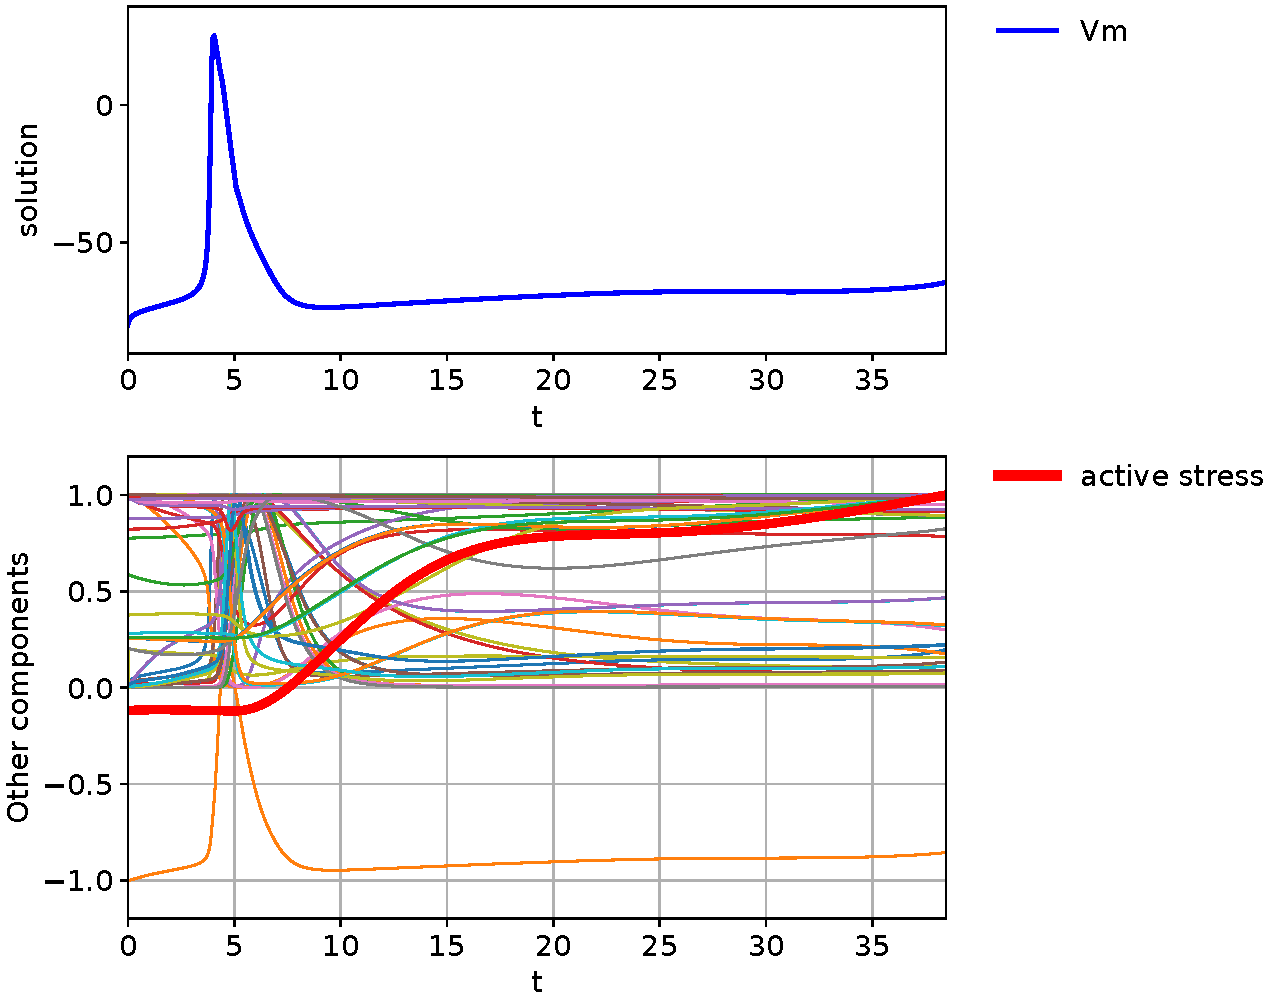
\includegraphics[width=0.8\textwidth]{images/results/basic/shorten_over_time.pdf}%
  \caption{Simulation of the Shorten subcellular model over time $t$ in milliseconds. The cell is stimulated at $t=\SI{5}{\ms}$. The upper plot shows the membrane voltage $V_m$, the lower plot show all other variables, some of which are listed in the legend on the right.}%
  \label{fig:shorten_over_time}%
\end{figure}%

In the upper plot, the depolarization and repolarization of the membrane can be seen upon the stimulation at $t=\SI{5}{\ms}$, exhibiting the characteristic action potential shape. The membrane voltage $V_m$ reaches its equilibrium value again at approximately $\SI{5}{\ms}$ after the stimulation. 
The lower plot in \cref{fig:shorten_over_time} shows longer durations for several other variables to return to the equilibrium state. As a consequence, the generated force or active stress of the sarcomeres, indicated by the thick red line in \cref{fig:shorten_over_time}, does not directly decrease after the stimulation is over. For frequent stimulation patterns, the force level would show a smooth progression over time.

The propagation of the action potentials of the Shorten subcellular model can be simulated with the monodomain equation (\cref{eq:monodomain}). \Cref{fig:shorten_03_50} shows according simulation results on a 1D muscle fiber mesh with length \SI{1}{\cm}, discretized to 100 elements. The muscle fiber is stimulated at its center at $t=0$. The upper plot in \cref{fig:shorten_03_50} displays the membrane voltage $V_m$ at time $t=\SI{3.5}{\ms}$. Two action potentials, which move towards both ends of the fiber can be identified. The lower plot shows all other variables, normalized to the value range $[-1,1]$. At the outer ends of the fiber, the variables are still in equilibrium, whereas towards the center, their values change dynamically as the action potentials propagate. 

% Shorten over mesh
\begin{figure}
  \centering%
  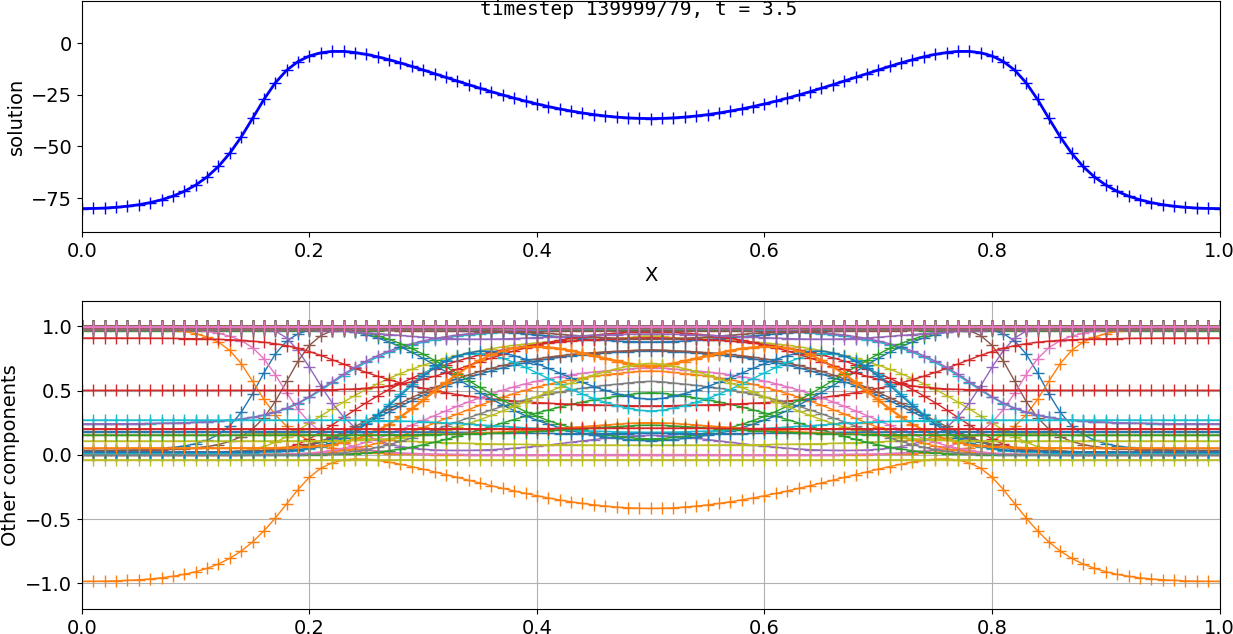
\includegraphics[width=0.8\textwidth]{images/results/basic/shorten_03_50.png}%
  \caption{Simulation of action potential propagation on a 1D mesh with the Shorten subcellular model. The upper plots shows the membrane voltage $V_m$ at time $t=\SI{3.5}{\ms}$ over the fiber along the $x$ axis. The lower plot shows all other variables of the model.}%
  \label{fig:shorten_03_50}%
\end{figure}%

\Cref{fig:hodgkin_huxley_over_mesh} shows analogous results for a simulation with the subcellular model of Hodgkin and Huxley \cite{Hodgkin1952}. Two action potentials can be seen  at time $t=\SI{4.25}{\ms}$ on a fiber mesh with 200 nodes and of \SI{2}{\cm} length. The system state is fully described by the values of the four variables that are plotted in \cref{fig:hodgkin_huxley_over_mesh}.

% Hodgkin_Huxley over mesh
\begin{figure}
  \centering%
  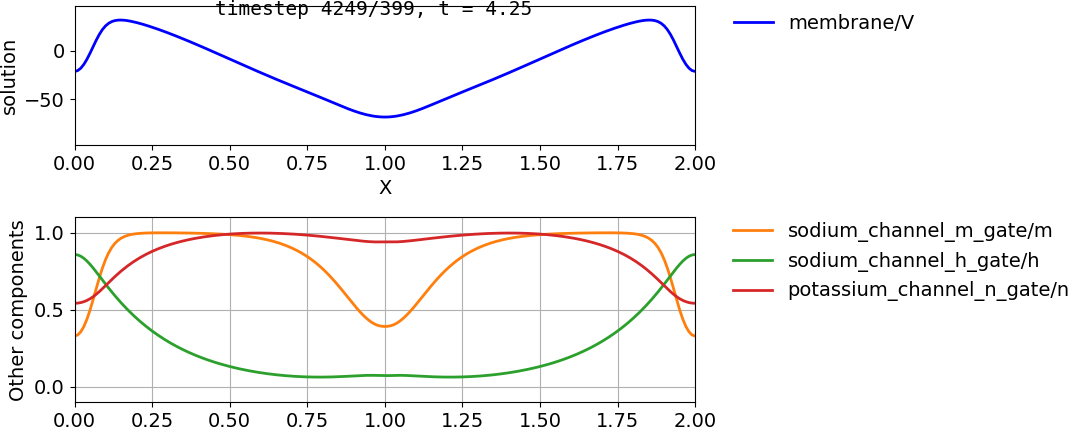
\includegraphics[width=0.9\textwidth]{images/results/basic/hodgkin_huxley_over_mesh.png}%
  \caption{Simulation of action potential propagation on a 1D mesh with the Hodgkin-Huxley subcellular model for time $t=\SI{4.25}{\ms}$, analogous to \cref{fig:shorten_03_50}.}%
  \label{fig:hodgkin_huxley_over_mesh}%
\end{figure}%

\begin{reproduce_no_break}
  The simulation of a single instance of the Shorten model and the plot of \cref{fig:shorten_over_time} can be obtained as follows:
  \begin{lstlisting}[columns=fullflexible,breaklines=true,postbreak=\mbox{\textcolor{gray}{$\hookrightarrow$}\space}]
    cd $\$$OPENDIHU_HOME/examples/electrophysiology/cellml/shorten/build_release
    ./cellml ../settings_cellml.py
    cd out && plot
  \end{lstlisting}
  The simulation of the monodomain equation for the Shorten model shown in \cref{fig:shorten_03_50} can be executed and visualized as follows: 
  \begin{lstlisting}[columns=fullflexible,breaklines=true,postbreak=\mbox{\textcolor{gray}{$\hookrightarrow$}\space}]
    cd $\$$OPENDIHU_HOME/examples/electrophysiology/monodomain/new_slow_TK_2014_12_08/build_release
    ./shorten_implicit ../settings_new_slow_TK_2014_12_08.py
    cd out && plot
  \end{lstlisting}
\end{reproduce_no_break}

\subsection{Simulation of Motoneuron Models}

If an activation model with a pool of motor neurons is considered in the neuromuscular multi-scale model, the transient behavior of motor neurons has to be simulated as well. In our simulations, we use the motor neuron model of Cisi and Kohn \cite{Cisi2008}. The drive parameter of the model is set to a constant value of \SI{0.01}{\volt\per\second}. In consequence, the motor neuron fires with a frequency that depends on the input drive, which in the presented scenario is approximately \SI{25}{\hertz}.

\Cref{fig:motoneuron_plot} shows the evolution of the different variables of the model over time. Six firing times can be identified. 

% Motoneuron over time
\begin{figure}
  \centering%
  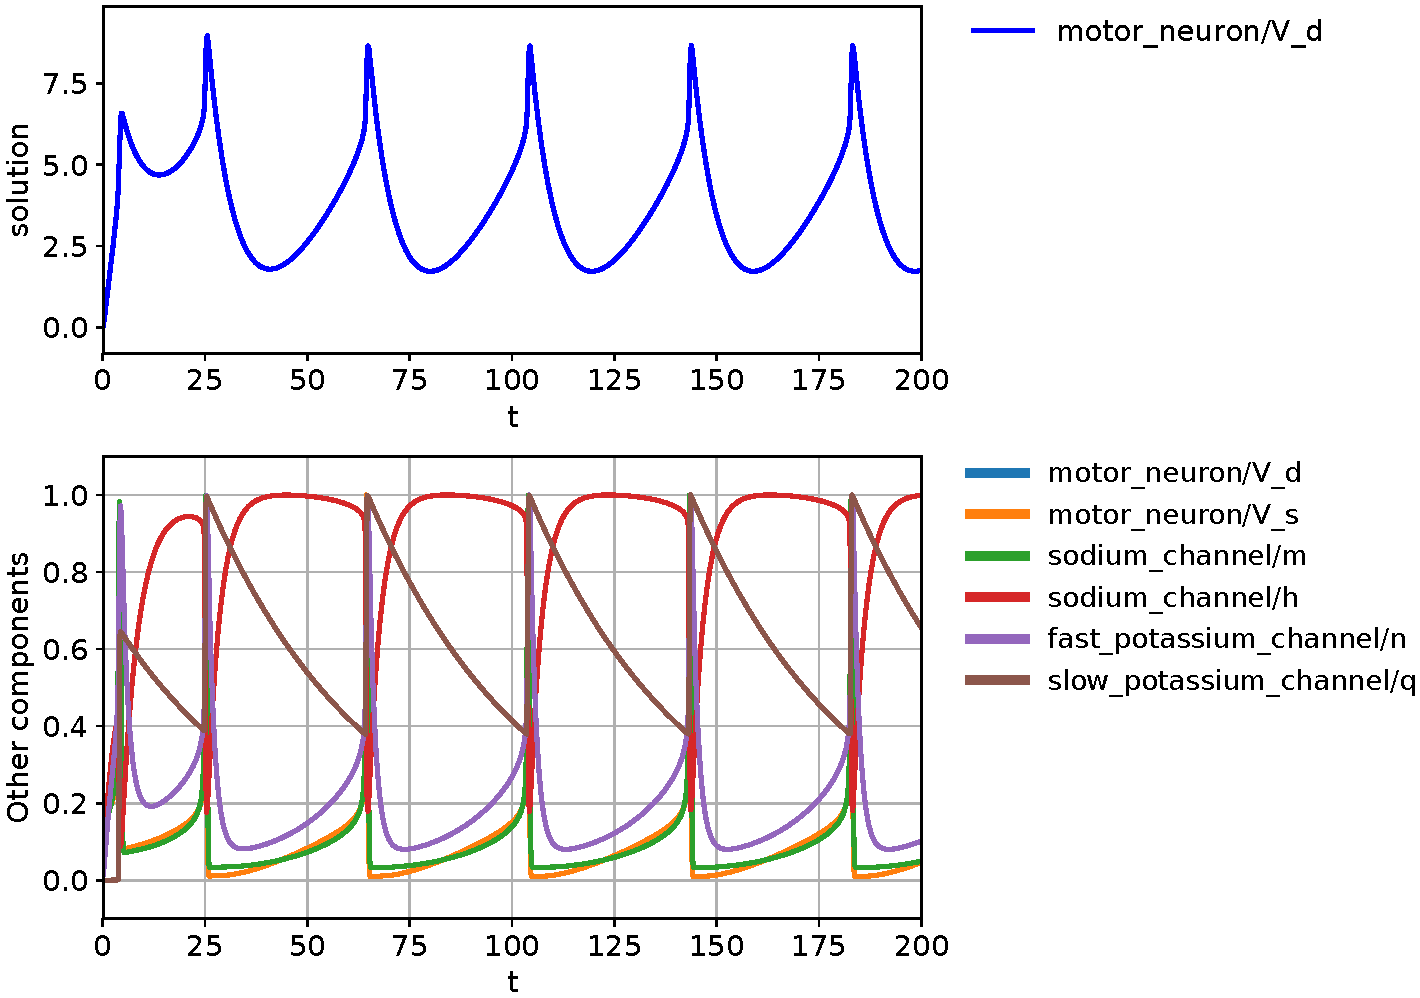
\includegraphics[width=\textwidth]{images/results/basic/motoneuron_plot.pdf}%
  \caption{Simulation of the motor neuron model of Cisi and Kohn \cite{Cisi2008} for a constant input drive of  \SI{0.01}{\volt\per\second}. The evolution of all variables of the model is plotted over time $t$ in milliseconds.}%
  \label{fig:motoneuron_plot}%
\end{figure}%

To connect the motor neuron with the fibers of the MU in the simulation, we stimulate the muscle fibers whenever the $V_s$ value of the motor neuron reaches a certain threshold. It is possible to configure a pool of several motor neurons with different model parameters and different input drive values. Each motor neuron can be connected to a different set of fibers, according to the MU to fiber association. In result, the MUs get physiologically activated according to the different firing frequencies of the motor neurons.

In summary, we showed simulations of the 0D subcellular models of Shorten et al. and Hodgkin and Huxley, simulations of these models together with the 1D conduction model in the monodomain equation, and a simulation of motor neurons. All of these models are given in CellML description and can be further combined with other parts of the multi-scale model, e.g., to simulate surface EMG signals.

\begin{reproduce_no_break}
  The simulation and visualization for \cref{fig:motoneuron_plot} can be executed with the following commands:
  \begin{lstlisting}[columns=fullflexible,breaklines=true,postbreak=\mbox{\textcolor{gray}{$\hookrightarrow$}\space}]
    cd $\$$OPENDIHU_HOME/examples/electrophysiology/monodomain/motoneuron_cisi_kohn/build_release
    ./motoneuron_cisi_kohn ../settings_motoneuron_cisi_kohn.py
    cd out && plot motoneuron*
  \end{lstlisting}
  This simulation also computes the monodomain equation one muscle fiber that gets activated whenever the motor neuron fires.
\end{reproduce_no_break}
%-----

% --------
%\fi
% f==============

% ==================
%\iffalse
% =-------------------

\section{Simulation of Fiber Based Electrophysiology}\label{sec:results_fiber_based_electrophysiology}
% ==================
%\iffalse
% =-------------------

In this section, we consider surface EMG signals on the upper arm by simulating the activation of the biceps brachii muscle. We use the fiber based multi-scale model consisting of 1D action potential propagation on muscle fibers, potentially involving a 0D subcellular model, and the 3D bidomain model.
In \cref{sec:overview_emg_simulation}, we introduce the setting of the simulation and present an examplary scenario to compute EMG signals.
Subsequently, we simulate various scenarios to investigate the effects of different model parameters and numerical settings on the resulting EMG signal. \Cref{sec:simfiber_mu} considers the effects of single motor units, \cref{sec:simfiber_fat} the fat layer, and \cref{sec:effects_of_the_mesh_width_emg} shows effects of the mesh width. \Cref{sec:simfiber_electrodes} presents a way to simulate realistic EMG electrodes and \cref{sec:simfiber_decomposition} deals with the decomposition of EMG signals.
In \cref{sec:sim_rosenfalck}, we describe our simulations with a phenomenological model for action potential propagation.

\subsection{Overview of the EMG Simulation}\label{sec:overview_emg_simulation}

% full_muscle_emg_raytrace_1.png
\begin{figure}
  \centering%
  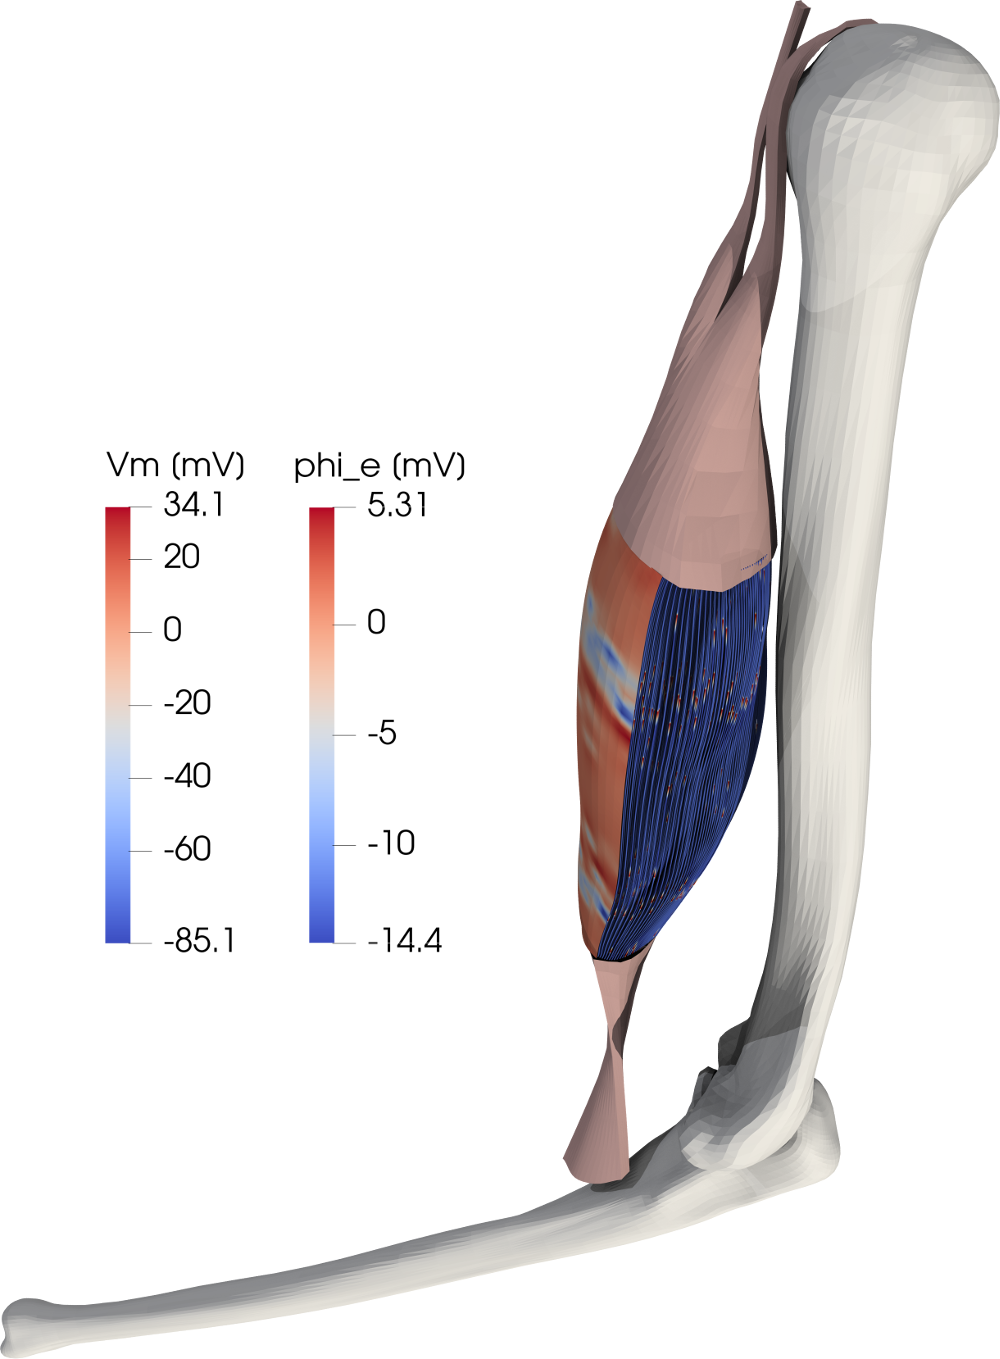
\includegraphics[width=0.6\textwidth]{images/results/application/full_muscle_emg_raytrace_1_small.png}%
  \caption{Considered setting for simulations of surface EMG for the upper arm, consisting of the biceps brachii muscle, tendons and bones. A simulation result of the membrane voltage $V_m$ on the muscle fibers and the extracellular potential $\phi_e$ on the surface is shown.}%
  \label{fig:full_muscle_emg_raytrace_1}%
\end{figure}

\Cref{fig:full_muscle_emg_raytrace_1} shows the setting of the biceps muscle and the tendons, which attach to the skeleton near the shoulder and to the ulna bone in the forearm. For the simulation of EMG, we only consider the muscle belly of the biceps muscle. \Cref{fig:full_muscle_emg_raytrace_1} shows muscle fibers inside the muscle, which run in longitudinal direction between the tendons at both ends. The image also visualizes the results of an EMG simulation. The fibers are colored according to the transmembrane potential $V_m$. On some fibers, action potentials can be seen.

The surface of the muscle is colored by the  extracellular electric potential $\phi_e$. In a reasonable approximation, the value of $\phi_e$ corresponds to the measured EMG signals on the skin surface. 
Additionally, we consider volume conduction in a layer of adipose tissue on top of the muscle in the following section.

For the EMG simulations, we solve the multi-scale model of fiber based electrophysiology. We solve the monodomain equation \cref{eq:monodomain} independently on all 1D muscle fiber meshes. 
After a fixed number of timesteps, we map the membrane voltage $V_m$ from the 1D meshes to the 3D mesh. Subsequently, we solve the static bidomain equation \cref{eq:bidomain1} on the muscle domain and potentially the body fat domain to obtain the $\phi_e$ values on the skin surface.

% fibers mesh
\begin{figure}
  \centering%
  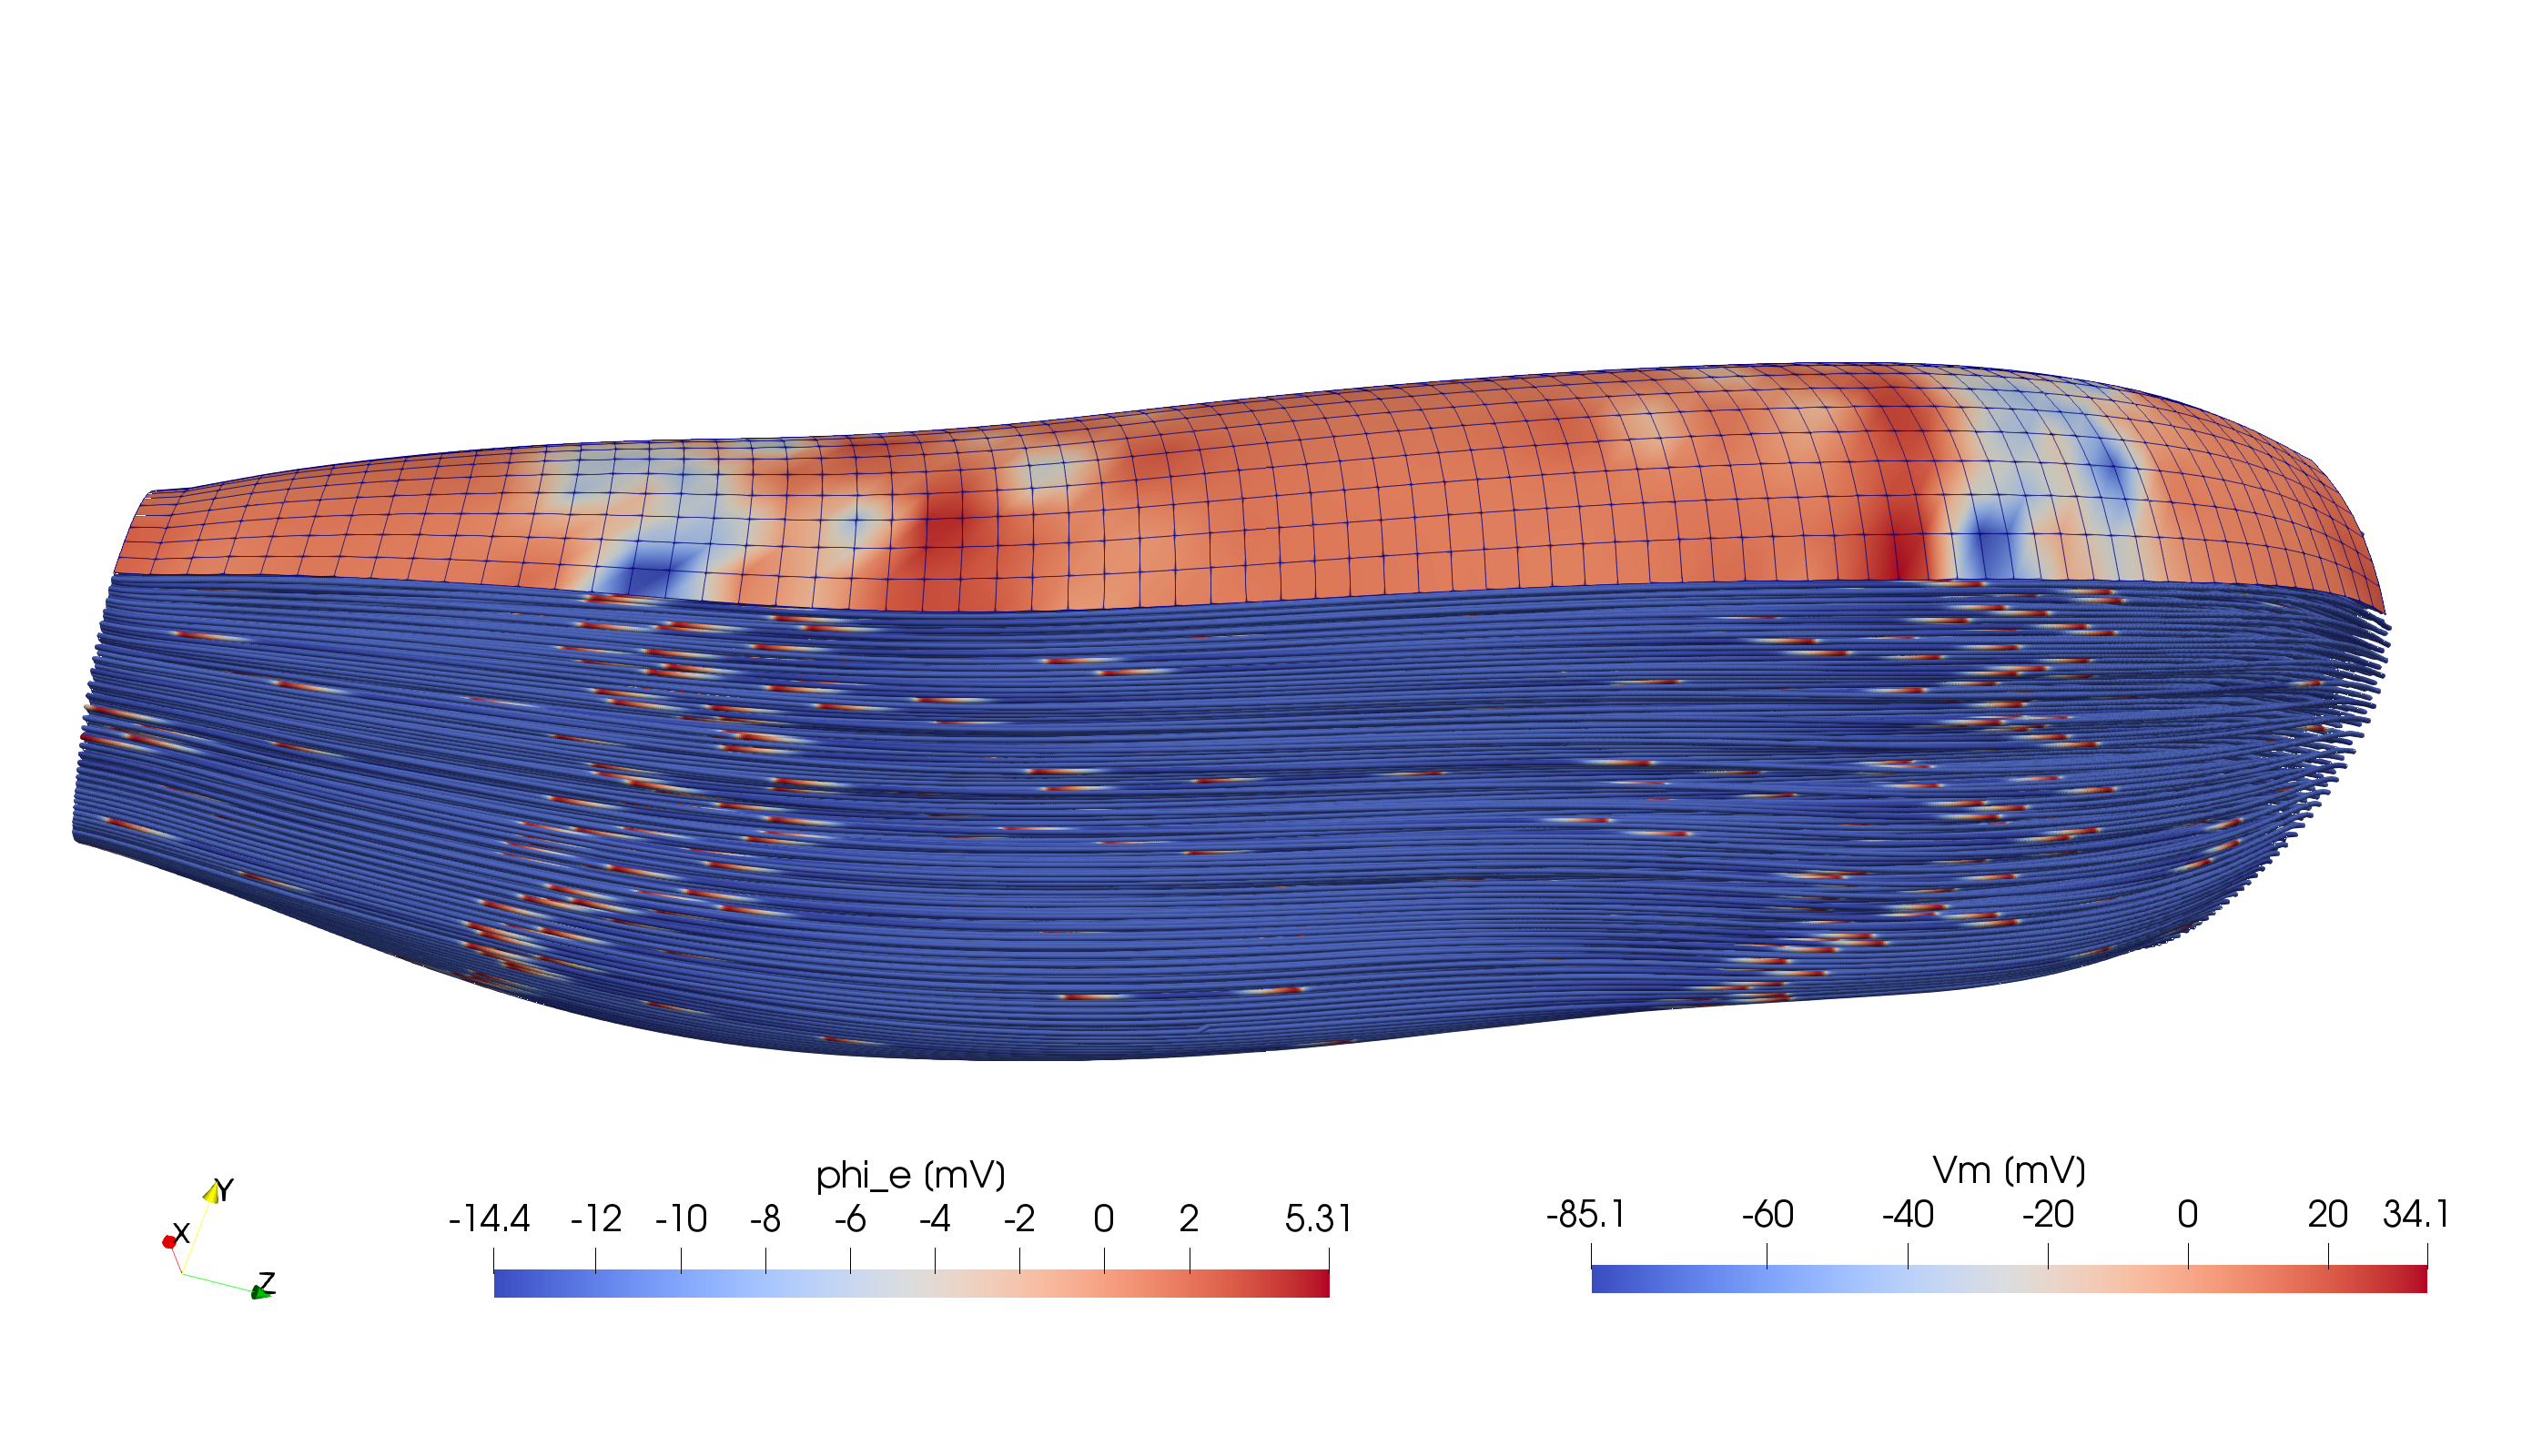
\includegraphics[width=\textwidth]{images/results/application/fibers_4.png}
  \caption{Overview of some of the meshes in an electrophysiology simulation: 1369 muscle fibers are located in the muscle belly. A 2D surface mesh on top of the muscle describes the computed EMG values. The visualized simulation is the same as in \cref{fig:full_muscle_emg_raytrace_1}.}%
  \label{fig:fibers_4}%
\end{figure}

\Cref{fig:fibers_4} shows a close-up view of the active muscle fibers and the resulting EMG signals on the upper surface, which are identical to \cref{fig:full_muscle_emg_raytrace_1}. The scenario considers 961 muscle fibers, each described by a 1D mesh with 1481 nodes. It can be seen that they are approximately equally spaced as a result of the meshing algorithms described in \cref{sec:generation_of_meshes_for_multiscale}.

\Cref{fig:fibers_4} also shows the mesh of the muscle surface, which is colored according to the extracellular potential $\phi_e$. It can be seen that the values correlate with the activation state of the underlying fibers. At the two blue colored regions at the surface near the left and right end of the muscle, the $\phi_e$ value is close to its minimum, while the majority of fibers exhibits its maximum positive $V_m$ value. Towards the center of the muscle, the value of $\phi_e$ increases to its maximum, which reflects the hyperpolarization of the muscle fibers behind the propagating action potentials, i.e., the overshoot of the membrane voltage before it reapproaches the equilibrium level.

The lower left corner in \cref{fig:fibers_4} shows the coordinate frame that is used in all simulations. The $z$ axis is approximately  oriented in fiber direction, the $x$ and $y$ axes are oriented in transverse direction and describe cross-sectional planes of the muscle.

The scenario uses the subcellular model of Hudgkin and Huxley \cite{Hodgkin1952}. The shown image corresponds to the simulation time of $t=\SI{200}{\milli\second}$. The simulation also considers a body fat mesh layer on top of the muscle, which is not visualized in \cref{fig:fibers_4}.

We run the simulation with 128 processes on a two-socket shared-memory node comprising two AMD EPYC 7742 64-core processors with \SI{2.87}{\giga\hertz} clock frequency and \SI{1.96}{\tebi\byte} RAM. The total runtime for a simulation end time of one second is \SI{8}{\hour} \SI{38}{\minute}.
%runtime: 8:37:44.43 on ipvs-epyc2

% scenario_name: 20mus_fibers,  n_subdomains: 4 1 32,  n_ranks: 128,  end_time: 1000.0
% dt_0D:           2.5e-03, diffusion_solver_type:      cg                                                                                                                                      
% dt_1D:           6.3e-04, potential_flow_solver_type: gmres                 
% dt_splitting:    2.5e-03, emg_solver_type:            cg, emg_initial_guess_nonzero: False
% dt_3D:           5.0e-01, paraview_output: True                                   
% output_timestep: 1.0e+00  stimulation_frequency: 0.1 1/ms = 100.0 Hz                                                                                                                          
% fast_monodomain_solver_optimizations: True, use_vc: True                                                                                                                                      
% fiber_file:              /data/scratch/sgs/maierbn/opendihu/examples/electrophysiology/input/left_biceps_brachii_31x31fibers.bin
% fat_mesh_file:           /data/scratch/sgs/maierbn/opendihu/examples/electrophysiology/input/left_biceps_brachii_31x31fibers.bin_fat.bin
% cellml_file:             /data/scratch/sgs/maierbn/opendihu/examples/electrophysiology/input/hodgkin_huxley_1952.c
% fiber_distribution_file: MU_fiber_distribution_31x31_10mus.txt
% firing_times_file:       /data/scratch/sgs/maierbn/opendihu/examples/electrophysiology/input/MU_firing_times_always.txt
% ********************************************************************************
% prefactor: sigma_eff/(Am*Cm) = 0.0132 = 3.828 / (500.0*0.58)
% n fibers:              961 (31 x 31)
% n points per fiber:    1481, sampled by stride 2 to 74
% 128 ranks, partitioning: x4 x y1 x z32
% 31 x 31 = 961 fibers, per partition: 7 x 31 = 217
% per fiber: 1D mesh    nodes global: 1481, local: 60
%   sampling 3D mesh with stride 2 x 2 x 20 (local_sampling_stride_z: 1)
%     linear 3D mesh    nodes global: 16 x 16 x 74 = 18944, local: 4 x 16 x 3 = 192
%     linear 3D mesh elements global: 15 x 15 x 73 = 16425, local: 4 x 15 x 3 = 180
% number of degrees of freedom:
%                     1D fiber:       1481  (per process: 60)
%             0D-1D monodomain:       5924  (per process: 240)
%  all fibers 0D-1D monodomain:    5692964  (per process: 52080)
%                  3D bidomain:      18944  (per process: 192)
%                        total:    5711908  (per process: 52272)
%     fat mesh, n points total:    6882 (31 x 3 x 74), (per process: 4 x 3 x 3 = 36)


\subsection{Effects of Single Motor Units on the Electromyography Signal}\label{sec:simfiber_mu}

Next, we investigate how the surface EMG signals are influenced by several parameters of the simulation. We begin by studying EMG of only a single activated MU in the muscle.

The first scenario contains 20 MUs that connect to an exponentially increasing number of fibers as shown in \cref{fig:MU_fibre_distribution_37x37_20c_txt_fiber_distribution}. The progression follows the function $y=c\,1.1^x$ for an appropriate constant $c>0$.
The MU assignment is created using method 1a of the algorithm described in \cref{sec:muscle_fibers_and_motor_units}, where the MU territories are centered around given points, and neighboring fibers are never part of the same MU. 

\Cref{fig:MU_fibre_distribution_37x37_20c_txt_2d_fiber_distribution} shows the fibers that are assigned to the smallest and to the largest MU, MU 1 and MU 20. For this visualization, the muscle cross-section is mapped to the large gray square and every colored small square corresponds to one fiber. The purple and red crosses indicate the center of the MU territories for MU 1 and 20, respectively. As a consequence, the fibers of MU 1 are mostly located at the bottom left of the cross-section and the fibers of MU 20 are mostly located in the upper right region of the muscle cross-section.
The visualization shows that the fibers of the same MU always have some spacing between them, which is due to the construction of the MU assignment algorithm.

% MU fiber sizes Vm
\begin{figure}[H]
  \centering%
  \begin{subfigure}[t]{\textwidth}%
    \centering%
    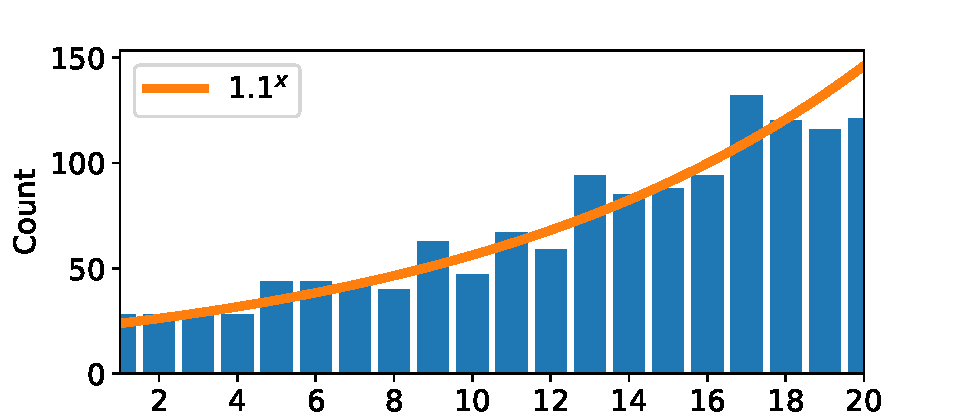
\includegraphics[width=0.6\textwidth]{images/results/application/MU_fibre_distribution_37x37_20c_txt_fiber_distribution_.pdf}%
    \caption{Exponential distribution of motor unit sizes. The diagram shows the motor unit numbers with the corresponding sizes or fibers counts of the MUs.}%
    \label{fig:MU_fibre_distribution_37x37_20c_txt_fiber_distribution}%
  \end{subfigure}\\
  \begin{subfigure}[t]{\textwidth}%
    \centering%
    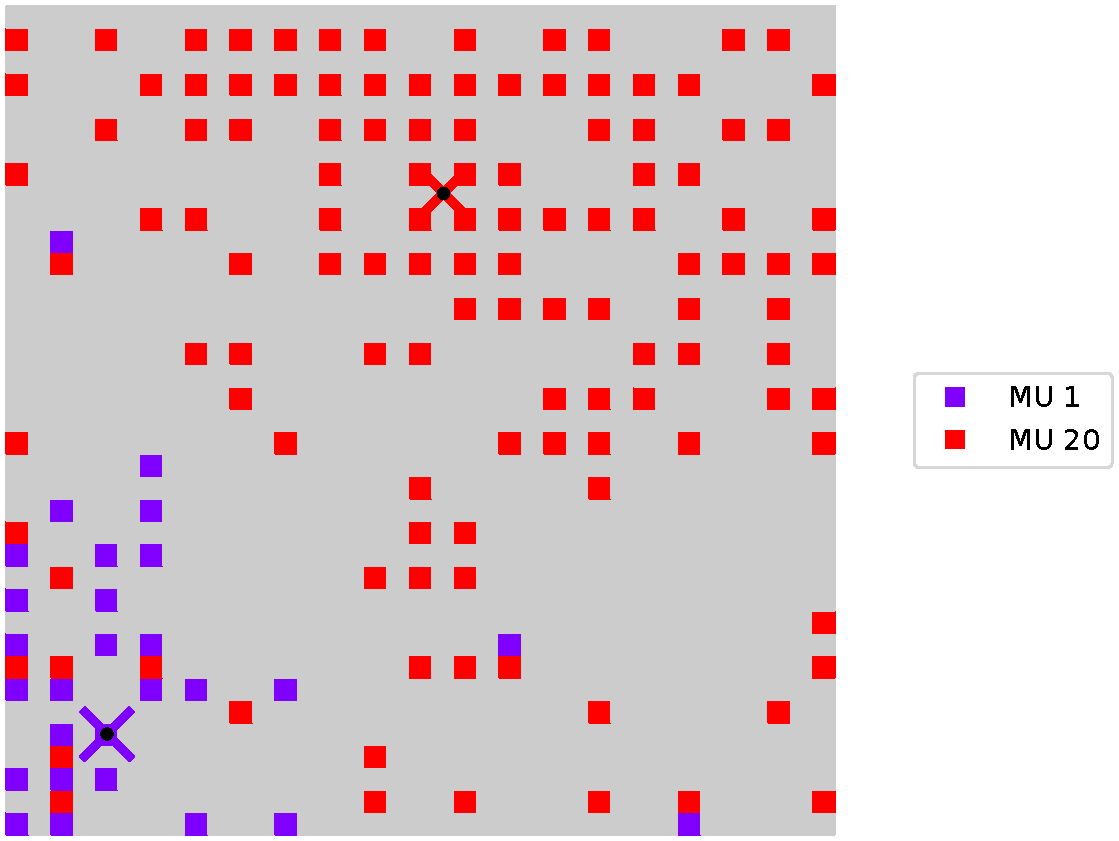
\includegraphics[width=0.6\textwidth]{images/results/application/MU_fibre_distribution_37x37_20c_txt_2d_fiber_distribution_.pdf}%
    \caption{Fibers that belong to motor units 1 and 20. The crosses are the center points around which the MU territories are generated by our algorithm.}%
    \label{fig:MU_fibre_distribution_37x37_20c_txt_2d_fiber_distribution}%
  \end{subfigure}
  \caption{Fiber based upper arm EMG simulation: Assignment of the 1369 fibres to 20 motor units used in the simulation scenario for fiber based electrophysiology.}%
  \label{fig:MU_fibre_distribution_37x37_20c}%
\end{figure}%

We begin with a simulation scenario, where only a single MU is stimulated, and study the effect on the surface EMG. The fibers of the respective MU are stimulated with a frequency $f=\SI{24}{\hertz}$ starting at time $t=\SI{0}{\milli\second}$. 
Each of the $13\times 13=\num{1369}$ fibers consists of a mesh with 1481 nodes, the 3D mesh of the muscle contains $19 \times 19 \times 38 = \num{13718}$ nodes and the 3D mesh of the fat layer contains $37 \times 5 \times 38 = \num{7030}$ nodes. The domains are partitioned into 27 subdomains associated to 27 MPI ranks. The subcellular model of Hodgkin and Huxley is used, yielding a total number of more than $\num{8.1e6}$ degrees of freedom. 
The timestep widths are $\dt_\text{0D}=\dt_\text{splitting} = \SI{2.5e-3}{\milli\second}$, $\dt_\text{1D} = \SI{6.25e-4}{\milli\second}$ and $\dt_\text{3D} = \SI{5e-1}{\milli\second}$, leading to 4 subcycles for the 1D model in each splitting step and 200 splitting steps per solution of the bidomain equation.

We compute the linear systems for the initial potential flow problem to estimate fiber directions in the 3D domain, \cref{eq:fiberest_laplace}, and for the bidomain equation \cref{eq:bidomain1}, which is solved in every timestep  using a conjugate gradient solver. 
The program uses the \code{FastMonodomainSolver} class for the electrophysiology model. The Thomas algorithm solves the linear system of the diffusion problem. We use the \code{`vc`} optimization type and employ the scheme to only compute active fibers and the subcellular problems that are not in equilibrium.

The computation of a simulated time span with $t_\text{end}=\SI{100}{\milli\second}$  on an AMD EPYC 7742 64-core processor with \SI{2492}{\mega\hertz} base frequency and \SI{1.96}{\tera\byte} RAM takes approximately $\SI{100}{\second}$ in the scenario that activates only the smallest MU, and $\SI{126}{\second}$ in the scenario that activates only the largest MU.

\Cref{fig:result_mu1} shows the result for the scenario of activating the smallest MU, MU 1. In \cref{fig:mu01a}, the surface is shown in the background and colored according to the extracellular potential $\phi_e$, which represents the EMG signal. The muscle volume is not shown. Instead, the active parts of the respective fibers are displayed as tubes in the 3D domain. Their color visualizes the value of the transmembrane voltage $V_m$. In every of these small tube segments, the rising and declining shape of an action potential can be observed by the color progression from blue over orange to red for the rising part and back to blue for the declining part.

In this scenario, the fibers of MU 1 are stimulated three times within the first $\SI{100}{\milli\second}$ at $\SI{0}{\milli\second}$, $\SI{41.6}{\milli\second}$ and $\SI{83.3}{\milli\second}$.  The innervation zone contains the starting points for the propagating stimulus on every fiber. The scenario positions the neuromuscular junctions randomly with a uniform distribution within the central $\SI{10}{\percent}$ of every muscle fiber. The activated parts of the fibers visible in \cref{fig:mu01a} correspond to the propagated action potentials of the last two stimulations in this scenario.

By comparing the results in \cref{fig:mu01a} with the fiber distribution in \cref{fig:MU_fibre_distribution_37x37_20c_txt_2d_fiber_distribution}, it can be seen that fibers of MU 1 are located opposite of the outer arm surface, which is at the upper side of the cross-sectional square diagram in \cref{fig:MU_fibre_distribution_37x37_20c_txt_2d_fiber_distribution}. The left side of the diagram in \cref{fig:MU_fibre_distribution_37x37_20c_txt_2d_fiber_distribution} corresponds to the lower part of the skin in \cref{fig:mu01a}. This part of the skin is closer to the activated fibers and, thus, the effect on the surface EMG is highest for this region.

\Cref{fig:mu01b} shows the skin surface as seen from the inside of the arm in \cref{fig:mu01a}. The active region is located at the right side in this image.
It can be seen that the active region on the skin surface, which results from fibers of the activated MU 1, only spans a small portion of the surface.

% Mu no. 1
\begin{figure}[H]
  \centering%
  \begin{subfigure}[t]{0.7\textwidth}%
    \centering%
    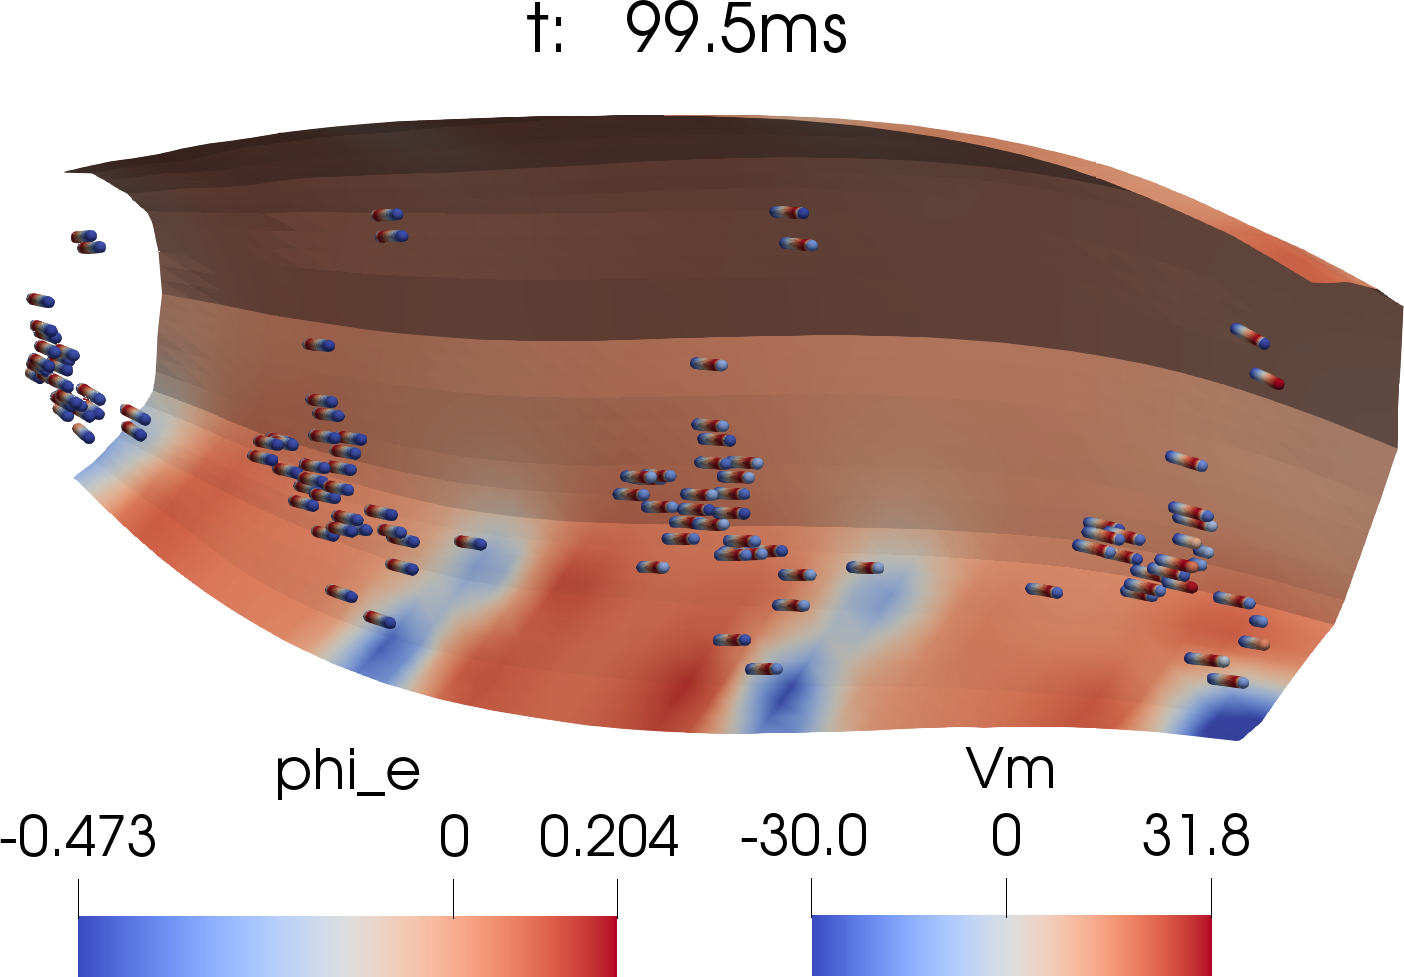
\includegraphics[width=\textwidth]{images/results/application/mu01a.png}%
    \caption{Membrane voltage $V_m$ at active parts of the fibers (foreground) and EMG signals $\phi_e$ on the skin surface (background).}%
    \label{fig:mu01a}%
  \end{subfigure} \,
  \begin{subfigure}[t]{0.25\textwidth}%
    \centering%
    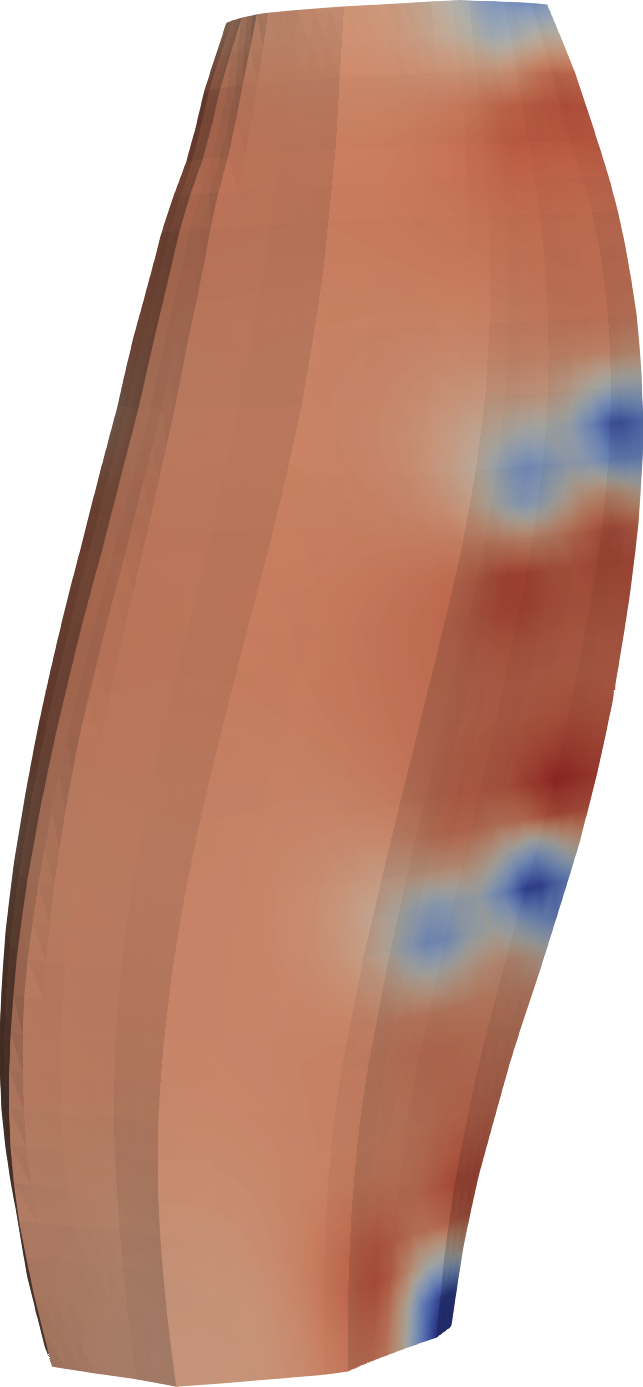
\includegraphics[width=\textwidth]{images/results/application/mu01b.png}%
    \caption{Resulting surface EMG.}%
    \label{fig:mu01b}%
  \end{subfigure}   
  \caption{Fiber based EMG simulation for the upper arm (biceps) model: Simulation result at $t=\SI{99.5}{\milli\second}$ where only MU 1 is activated.}%
  \label{fig:result_mu1}%
\end{figure}%

% Mu no. 20
\begin{figure}[H]
  \centering%
  \begin{subfigure}[t]{0.7\textwidth}%
    \centering%
    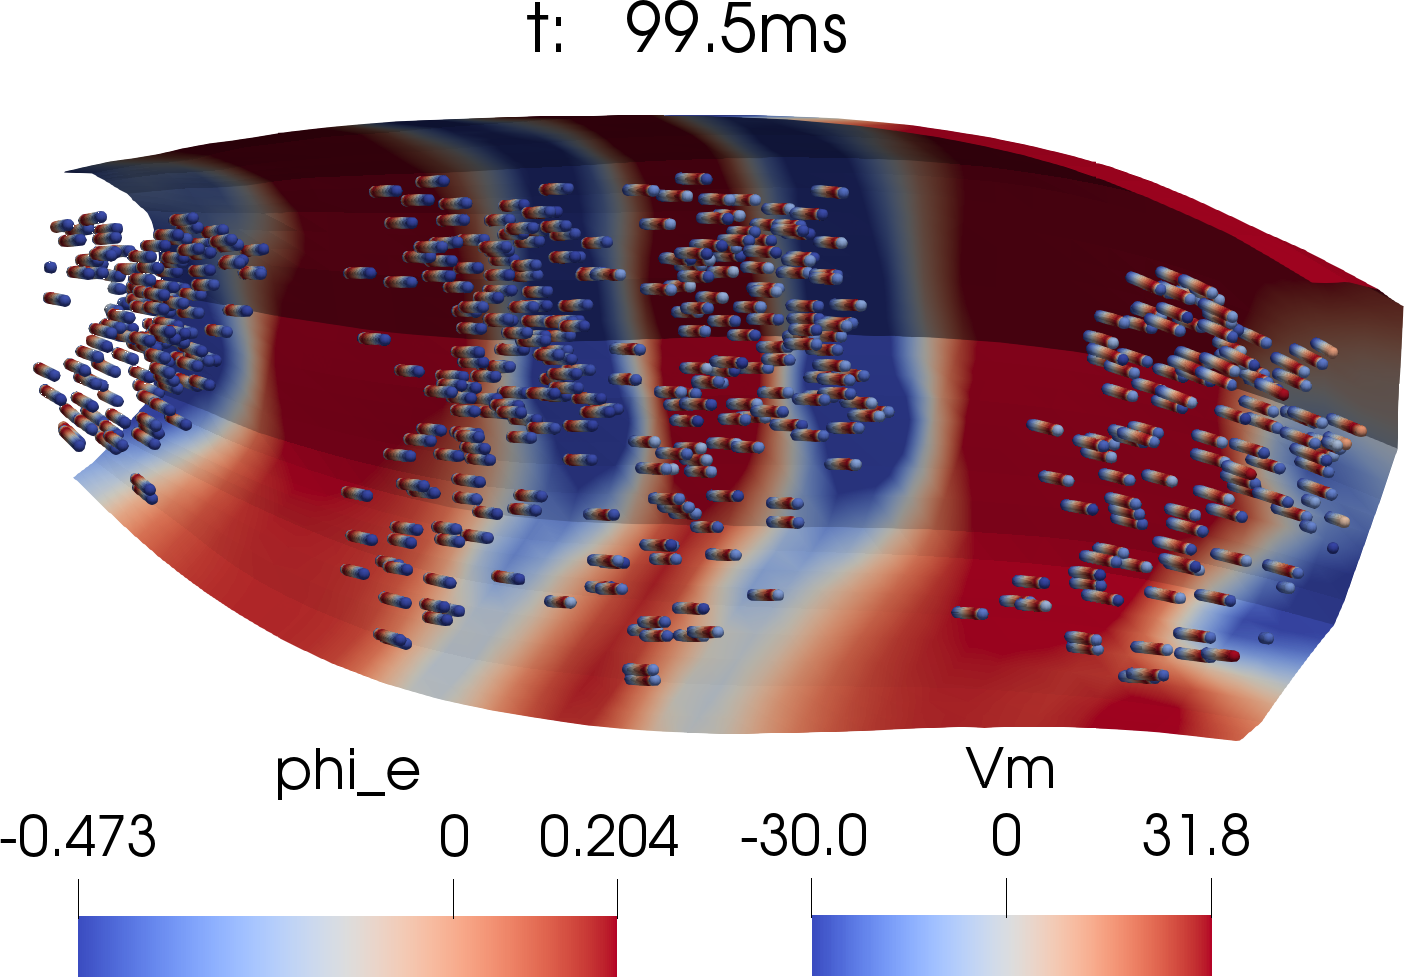
\includegraphics[width=\textwidth]{images/results/application/mu20a.png}%
    \caption{Membrane voltage $V_m$ at active parts of the fibers (foreground) and EMG signals $\phi_e$ on the skin surface (background).}%
    \label{fig:mu20a}%
  \end{subfigure} \,
  \begin{subfigure}[t]{0.25\textwidth}%
    \centering%
    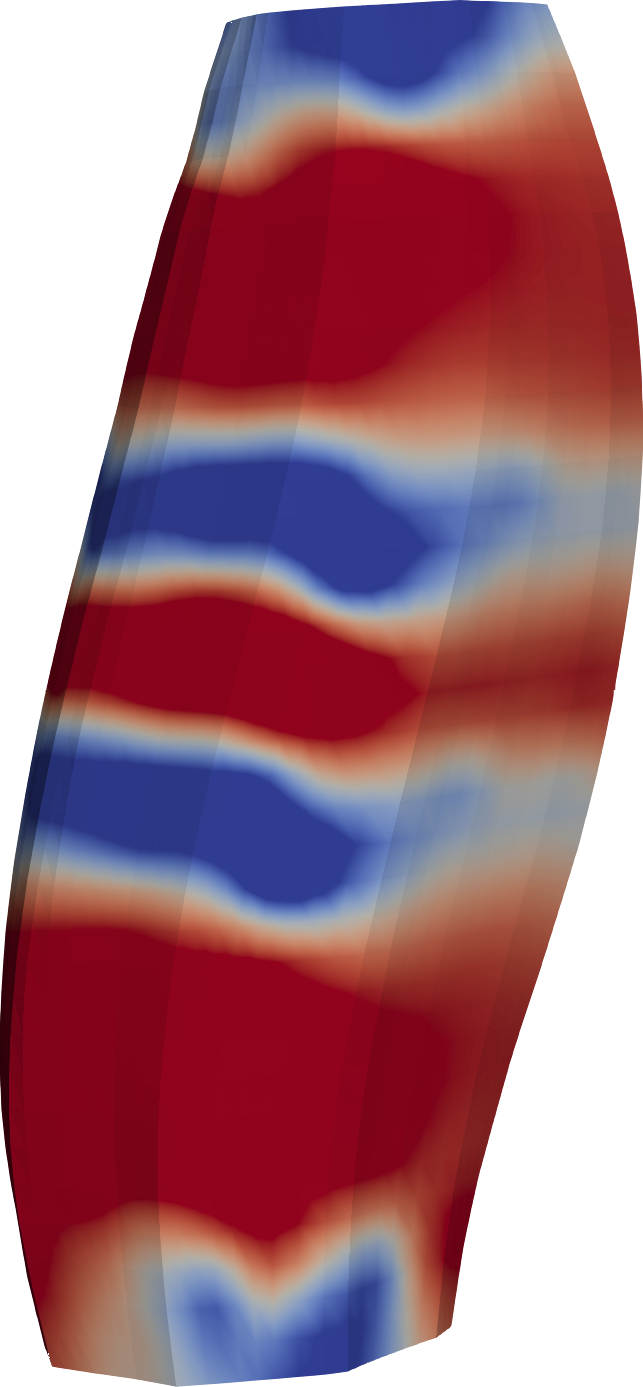
\includegraphics[width=\textwidth]{images/results/application/mu20b.png}%
    \caption{Resulting surface EMG.}%
    \label{fig:mu20b}%
  \end{subfigure}   
  \caption{Fiber based EMG simulation for the upper arm (biceps) model: Simulation result at $t=\SI{99.5}{\milli\second}$ where only motor unit 20 is activated, analogous to \cref{fig:result_mu1}.}%
  \label{fig:result_mu20}%
\end{figure}%

\Cref{fig:result_mu20} shows the analoguous scenario that activates MU 20 instead of MU 1. \Cref{fig:mu20a} shows that, now, more fibers are activated as MU 20 is larger than MU 1. According to the MU layout in \cref{fig:MU_fibre_distribution_37x37_20c_txt_2d_fiber_distribution}, the active fibers are also located closer to the skin surface. This layout results in a stronger EMG signal compared to the previous scenario. 

The color coding in the two scenarios in \cref{fig:result_mu1,fig:result_mu20} is identical and it can be seen that the absolute value of the extracellular potential $\phi_e$ is larger in the scenario for MU 20. For the scenario with MU 1 in \cref{fig:result_mu1}, the value range of the extracellular potential $\phi_e$ is $[\SI{-0.473}{\milli\volt}, \SI{0.204}{\milli\volt}]$. For the scenario with MU 20 in \cref{fig:result_mu20}, it is $[\SI{-0.834}{\milli\volt}, \SI{0.579}{\milli\volt}]$, which is more than twice the range.

\Cref{fig:mu20b} shows the overall EMG signal on the skin surface for MU 20. Compared to the result of MU 1 in \cref{fig:mu01b}, nearly the inverse region is activated. It can, thus, be observed that the EMG signal is highly influenced by the location and size of the MUs. MUs with territories closer to the skin surface have a larger effect on the EMG signals than MUs that are located further away. As seen in \cref{fig:mu01b}, the influence of fibers completely vanishes if the distance is larger than a certain value. The effects of several close fibers add up, such that large MUs located near the surface have the largest impact on the resulting EMG signal.

% 0/27 : This is opendihu 1.2, built Apr  2 2021, C++ 201402, GCC 10.2.0, current time: 2021/4/2 22:05:20, hostname: ipvs-epyc2, n ranks: 27
% 0/27 : Open MPI v3.1.6, package: Open MPI maierbn@ipvs-epyc1 Distribution, ident: 3.1.6, repo rev: v3.1.6, Mar 18, 2020
% 0/27 : File "/data/scratch/sgs/maierbn/opendihu/examples/electrophysiology/fibers/fibers_fat_emg/settings_fibers_fat_emg.py" loaded.
% 0/27 : ---------------------------------------- begin python output ----------------------------------------
% Loading variables from "20mus_activate_one_mu.py".                                             
% MU 0                                                                                           
%   radius: 40.0                                                                                 
%   cm: 0.58                                                                                     
%   activation_start_time: 10000                                                                 
%   stimulation_frequency: 24                                                                    
% MU 4                                                                                           
%   radius: 42.7067691737                                                                        
%   cm: 0.58                                                                                     
%   activation_start_time: 10000                                                                 
%   stimulation_frequency: 24                                                                    
% MU 8                                                                                           
%   radius: 45.63666317700952                                                                    
%   cm: 0.58                                                                                     
%   activation_start_time: 10000                                                                 
%   stimulation_frequency: 24                                                                    
% MU 12                                                                                          
%   radius: 48.80807467158288
%   cm: 0.58                                     
%   activation_start_time: 10000
%   stimulation_frequency: 24
% MU 16                                          
%   radius: 52.24091246590275
%   cm: 1.0                                      
%   activation_start_time: 10000
%   stimulation_frequency: 24
% scenario_name: 20mus_activate_only_mu_20,  n_subdomains: 3 1 9,  n_ranks: 27,  end_time: 100.0
% dt_0D:           2.5e-03, diffusion_solver_type:      cg
% dt_1D:           6.3e-04, potential_flow_solver_type: gmres
% dt_splitting:    2.5e-03, emg_solver_type:            cg, emg_initial_guess_nonzero: False
% dt_3D:           5.0e-01, paraview_output: True 
% output_timestep: 1.0e+00  stimulation_frequency: 0.1 1/ms = 100.0 Hz
% fast_monodomain_solver_optimizations: True, use_vc: True
% fiber_file:              /data/scratch/sgs/maierbn/opendihu/examples/electrophysiology/input/left_biceps_brachii_37x37fibers.bin
% fat_mesh_file:           /data/scratch/sgs/maierbn/opendihu/examples/electrophysiology/input/left_biceps_brachii_37x37fibers.bin_fat.bin
% cellml_file:             ../../../input/hodgkin_huxley_1952.c
% fiber_distribution_file: fiber_distribution/MU_fibre_distribution_37x37_20c.txt
% firing_times_file:       /data/scratch/sgs/maierbn/opendihu/examples/electrophysiology/input/MU_firing_times_always.txt
% ********************************************************************************
% prefactor: sigma_eff/(Am*Cm) = 0.0132 = 3.828 / (500.0*0.58)
% n fibers:              1369 (37 x 37), sampled by stride 2 x 2
% n points per fiber:    1481, sampled by stride 40
% 27 ranks, partitioning: x3 x y1 x z9                                                           
% 37 x 37 = 1369 fibers, per partition: 12 x 36 = 432                                            
% per fiber: 1D mesh    nodes global: 1481, local: 200                                                                                                                                          
%   sampling 3D mesh with stride 2 x 2 x 40                                                                                                                                                     
%     linear 3D mesh    nodes global: 19 x 19 x 38 = 13718, local: 6 x 19 x 5 = 570                                                                                                             
%     linear 3D mesh elements global: 18 x 18 x 37 = 11988, local: 6 x 18 x 5 = 540                                                                                                             
% number of degrees of freedom:                                                                  
%                     1D fiber:       1481  (per process: 200)                                   
%             0D-1D monodomain:       5924  (per process: 800)                                   
%  all fibers 0D-1D monodomain:    8109956  (per process: 345600)                                
%                  3D bidomain:      13718  (per process: 570)                                   
%                        total:    8123674  (per process: 346170)                                
%     fat mesh, n points total:    7030 (37 x 5 x 38), (per process: 6 x 5 x 5 = 150)            
% Debugging output about fiber firing: Taking input from file "/data/scratch/sgs/maierbn/opendihu/examples/electrophysiology/input/MU_firing_times_always.txt"
% First stimulation times                                      

\subsection{Effects of the Fat Layer on the Electromyography Signal}\label{sec:simfiber_fat}

% different fat meshes
\begin{figure}[H]
  \centering%
  \begin{subfigure}[t]{0.3\textwidth}%
    \centering%
    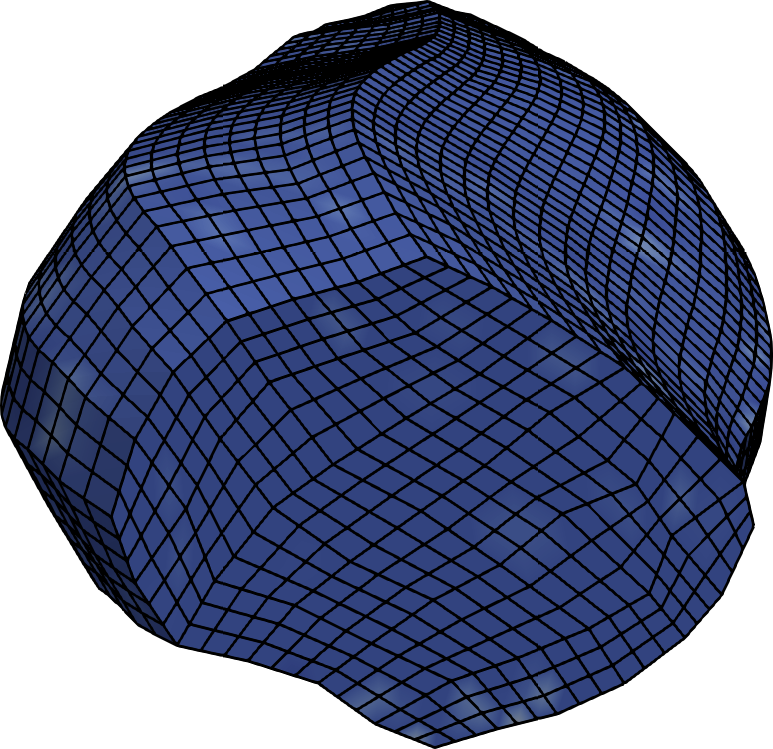
\includegraphics[width=\textwidth]{images/results/application/fibers_emg_mesh_no_fat.png}%
    \caption{Muscle mesh without fat layer.}%
    \label{fig:fibers_emg_mesh_no_fat}%
  \end{subfigure} \quad
  \begin{subfigure}[t]{0.3\textwidth}%
    \centering%
    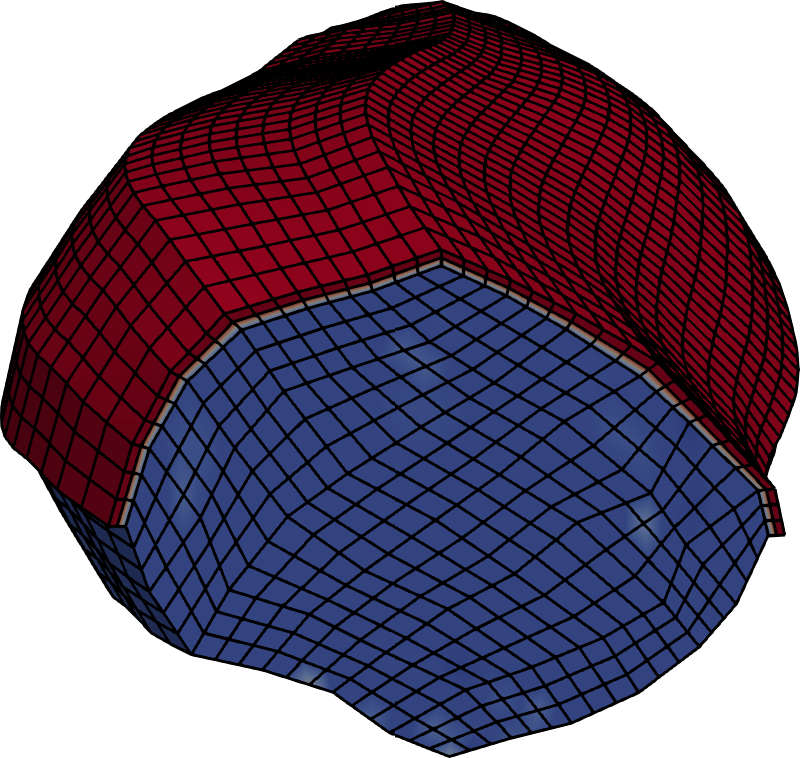
\includegraphics[width=\textwidth]{images/results/application/fibers_emg_mesh_thin_fat.png}%
    \caption{Muscle with thin fat layer.}%
    \label{fig:fibers_emg_mesh_thin_fat}%
  \end{subfigure}  \quad
  \begin{subfigure}[t]{0.3\textwidth}%
    \centering%
    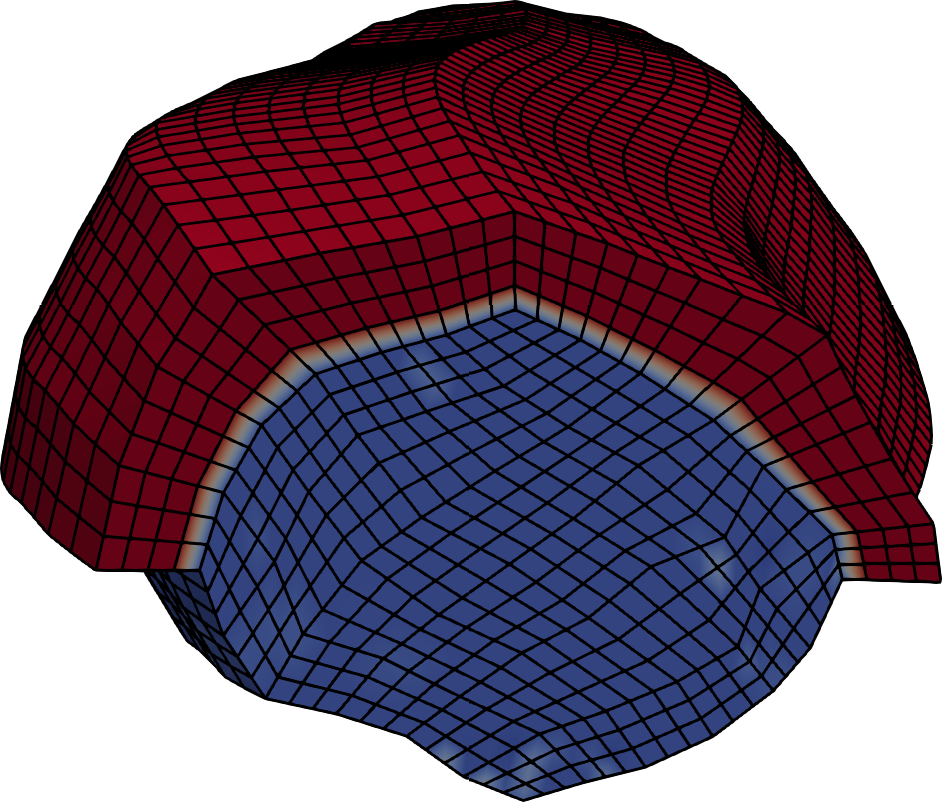
\includegraphics[width=\textwidth]{images/results/application/fibers_emg_mesh_thick_fat.png}%
    \caption{Muscle with thick fat layer.}%
    \label{fig:fibers_emg_mesh_thick_fat}%
  \end{subfigure}   
  \caption{Fiber based EMG simulation for the upper arm (biceps) model: Meshes for the muscle domains (blue) and the layer of adipose tissue (red) used in the study to compare different fat layer widths.}%
  \label{fig:fibers_emg_mesh_fat}%
\end{figure}%

In the next study, we investigate the effect of the fat layer on the resulting EMG signals. The same scenario as in the previous section is used, except that the size of the body fat domain is varied and the activated MUs are chosen differently. We consider the domains and meshes shown in \cref{fig:fibers_emg_mesh_fat}: Scenario (a) only considers the muscle domain without additional  fat layer. Scenario (b) adds a thin fat layer with thickness of $\SI{2}{\milli\meter}$, discretized by two layers of finite elements. Scenario (c) considers a fat layer with thickness of $\SI{1}{\centi\meter}$ and four layers of elements. The scenario in the previous section also used this thick fat layer.

In this series of experiments, the first 10 MUs are activated with different stimulation frequencies ranging from \SI{7}{\hertz} for the smallest MU to \SI{15.15}{\hertz} for MU 10. The runtime of the simulation for one scenario on the same hardware as in the previous section is approximately $\SI{9}{\minute}$.

\Cref{fig:fibers_emg_fat} shows the simulation results at $t=\SI{100}{\milli\second}$ for the three scenarios with different fat layers. The figure uses the same color coding for the extracellular potential $\phi_e$ in all three scenarios. It can be seen that the volume conduction in the fat layer significantly smooths the resulting EMG signal, especially for the thick fat layer. The scenarios with no fat layer and the thin fat layer also exhibit a small difference.
This effect has implications for experimental studies, where the EMG recordings capture the less resolved spatial information, the more tissue is located between the muscle and the surface electrodes.

% results for different fat meshes
\begin{figure}[H]
  \centering%
  \begin{subfigure}[t]{0.36\textwidth}%
    \centering%
    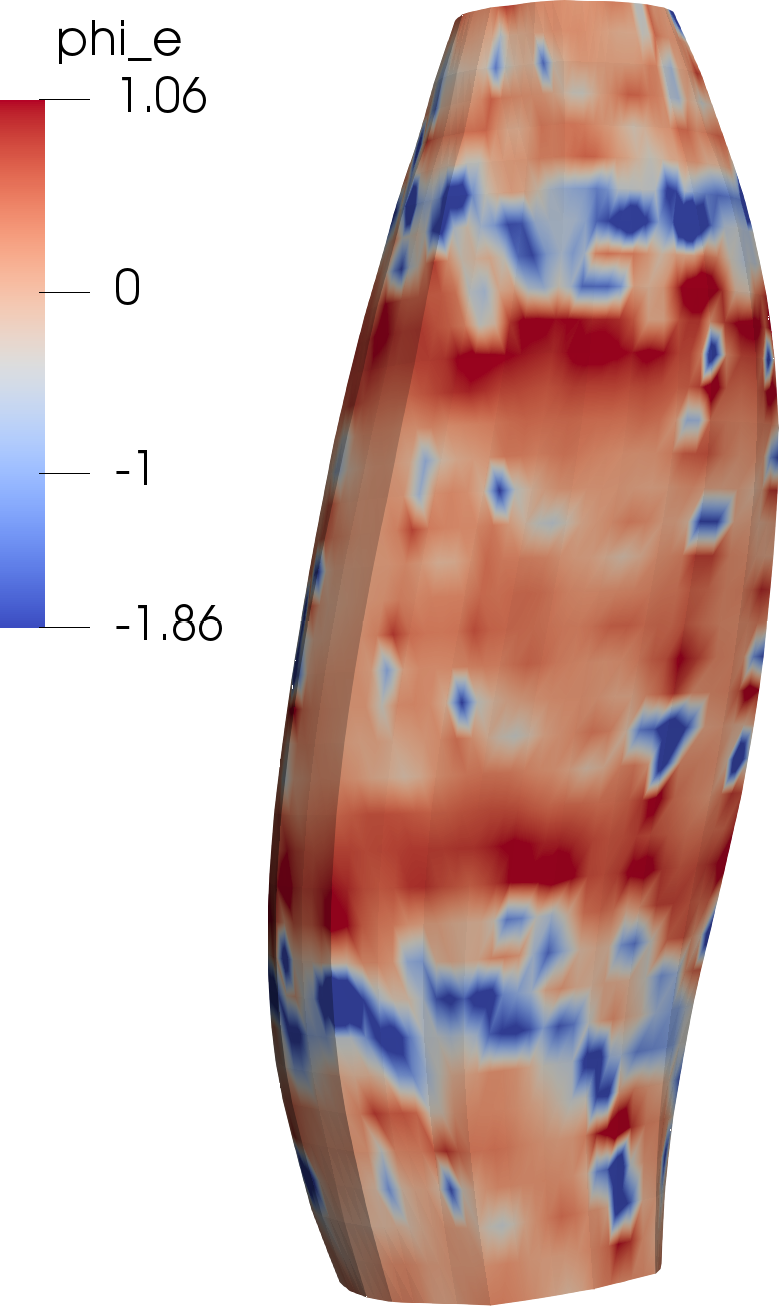
\includegraphics[width=\textwidth]{images/results/application/fibers_emg_no_fat.png}%
    \caption{Simulation without fat layer.}%
    \label{fig:fibers_emg_no_fat}%
  \end{subfigure} \quad
  \begin{subfigure}[t]{0.25\textwidth}%
    \centering%
    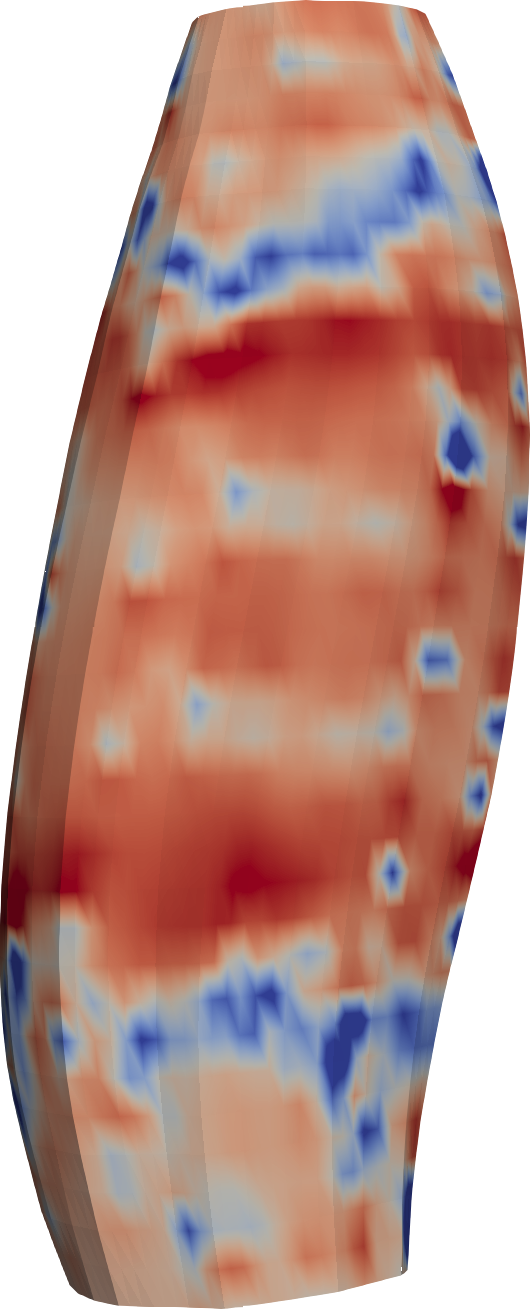
\includegraphics[width=\textwidth]{images/results/application/fibers_emg_thin_fat.png}%
    \caption{Simulation with a thin fat layer.}%
    \label{fig:fibers_emg_thin_fat}%
  \end{subfigure}  \quad
  \begin{subfigure}[t]{0.28\textwidth}%
    \centering%
    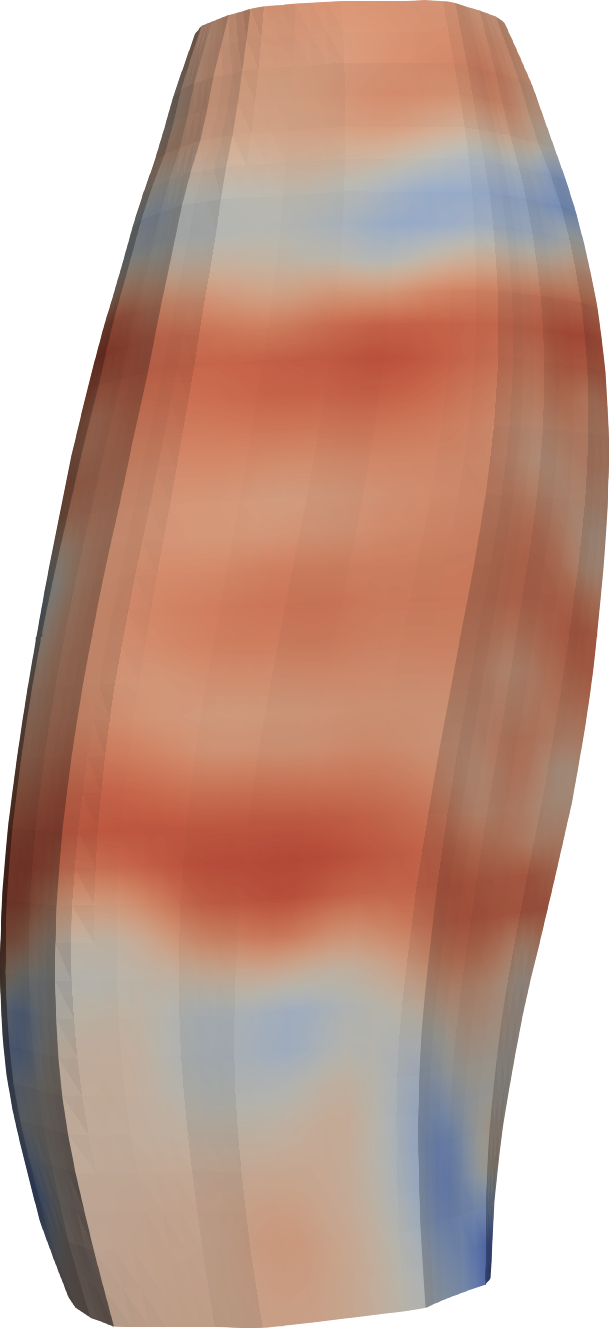
\includegraphics[width=\textwidth]{images/results/application/fibers_emg_thick_fat.png}%
    \caption{Simulation with a thick fat layer.}%
    \label{fig:fibers_emg_thick_fat}%
  \end{subfigure}   
  \caption{Fiber based EMG simulation for the upper arm (biceps) model: Simulated surface EMG signals for the different fat layers shown in \cref{fig:fibers_emg_mesh_fat}.}%
  \label{fig:fibers_emg_fat}%
\end{figure}%

\begin{reproduce}
  The simulations in this section use the examples \code{examples/electrophysiology/fibers/fibers_emg} and \code{examples/electrophysiology/fibers/fibers_fat_emg} with the variables file \code{20mus_fat_comparison.py}.

  The scenario data that are necessary to run the simulations are given in the repository at \href{https://github.com/dihu-stuttgart/performance}{github.com/dihu-stuttgart/performance}
  in the directory \code{opendihu/}\code{18_fibers_emg}. The main scripts that runs the simulations for the two sections are the following:
  \begin{lstlisting}[columns=fullflexible,breaklines=true,postbreak=\mbox{\textcolor{gray}{$\hookrightarrow$}\space}]
    ./run_single_MUs.sh
    ./run_compare_fat_layer.sh
  \end{lstlisting}
\end{reproduce}


\subsection{Effects of the Mesh Width on the Electromyography Signal}\label{sec:effects_of_the_mesh_width_emg}

% Hier herausarbeiten, dass das eine sehr wichtige Frage für Deine Arbeit ist, quasi die Rechtfertigung, dass man hohe Auflösungen braucht oder: Ziel der Arbeit war unter anderem, hetauszufinden, wieviel qualitativ und quantitativ neue Effekte sichtbar werden, wenn die Auflösung hoch genug ist. 
% Evtl. sollte man hier auch nochmal erwähnen, wie viele Fasern ein durchschittlicher Bizeps in der Realität hat?

One goal of our simulation studies is to evaluate the required mesh width and the necessary number of fibers to obtain accurate simulation results of surface EMG signals.
Experimental studies reveal a large variation in the number of muscle fibers in a real biceps brachii muscle. MacDougall et al. estimate in vivo numbers for elite and intermediate bodybuilders and untrained control subjects and find comparable numbers for these groups \cite{MacDougall1984}. They determine $278.5 \pm 60.7 \times \num{1e3}$ muscle fibers for the group untrained subjects.
Thus, we simulate scenarios with different 3D mesh resolutions and numbers of fibers up to the realistic number of \num{273529}. By comparing the obtained simulation results, we can determine if certain effects are only visible for high resolutions.

We consider a scenario with 100 MUs and increase the spatial resolution and the number of processes that execute the computation on the supercomputer Hawk at the High Performance Computing Center Stuttgart. Each compute node consists of two two AMD EPYC 7742 processors with 64 cores each, a clock frequency of \SI{2.25}{\giga\hertz} and \SI{256}{\giga\byte} memory per node.

% fibers mesh
\begin{figure}
  \centering%
  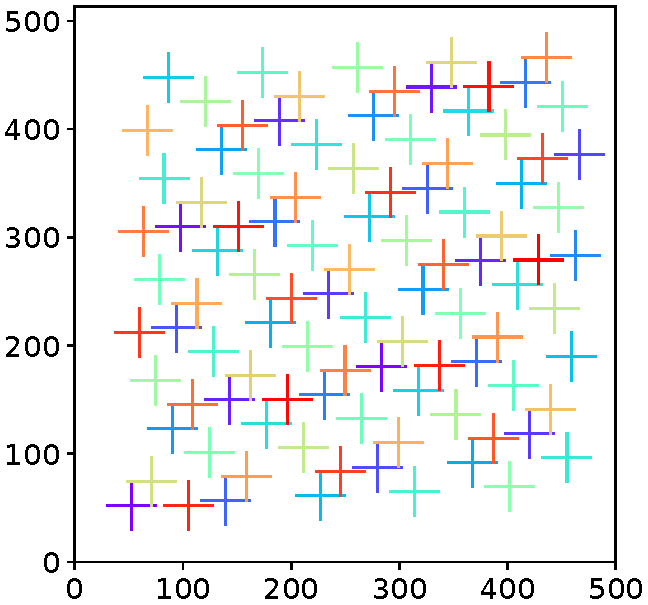
\includegraphics[width=0.5\textwidth]{images/results/application/MU_fibre_distribution_523x523_100mus_txt_mu_positions.pdf}%
  \caption{Fiber based EMG simulation for the upper arm (biceps) model; study of different mesh widths, MU territory center points. The shown center points of the 100 motor units are used in all different scenarios within the study of different mesh widths.}%
  \label{fig:MU_fibre_distribution_523x523_100mus_txt_mu_positions}%
\end{figure}

Our simulated scenarios consider between \num{1369} and \num{273529} fibers. The specified number of 100 MUs has to be assigned to these numbers of fibers for each scenario.
We use the method 1a of the algorithm described in \cref{sec:muscle_fibers_and_motor_units}. The MU territories are centered around quasi-randomly generated center points, as shown in \cref{fig:MU_fibre_distribution_523x523_100mus_txt_mu_positions}. It can be seen that the MU territory center points are homogeneously distributed in space.


% MU distributions
\begin{figure}
  \centering%
  \begin{subfigure}[t]{0.45\textwidth}%
    \centering%
    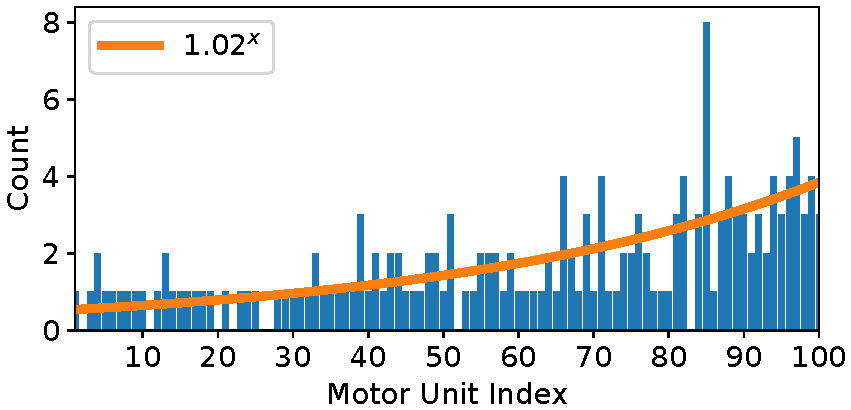
\includegraphics[width=\textwidth]{images/results/application/MU_fibre_distribution_13x13_100mus_txt_fiber_distribution.pdf}%
    \caption{Size distribution for $13\times 13 = 169$ fibers.}%
    \label{fig:mus_13}%
  \end{subfigure} \quad
  \begin{subfigure}[t]{0.45\textwidth}%
    \centering%
    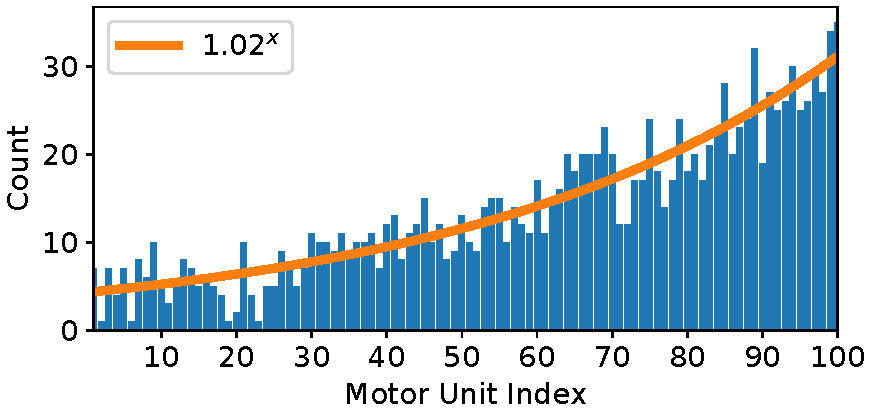
\includegraphics[width=\textwidth]{images/results/application/MU_fibre_distribution_37x37_100mus_txt_fiber_distribution.pdf}%
    \caption{Size distribution for $37\times 37 = 1369$ fibers.}%
    \label{fig:mus_37}%
  \end{subfigure}  \\
  \begin{subfigure}[t]{0.45\textwidth}%
    \centering%
    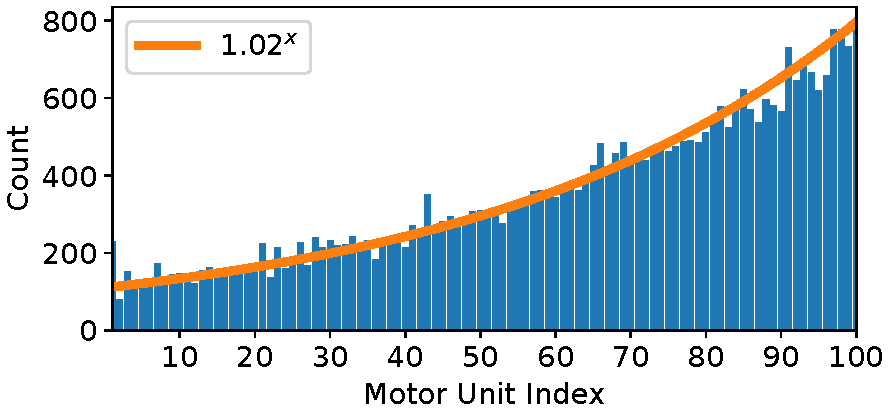
\includegraphics[width=\textwidth]{images/results/application/MU_fibre_distribution_187x187_100mus_txt_fiber_distribution.pdf}%
    \caption{Size distribution for $187\times 187 = \num{34969}$ fibers.}%
    \label{fig:mus_187}%
  \end{subfigure} 
  \begin{subfigure}[t]{0.45\textwidth}%
    \centering%
    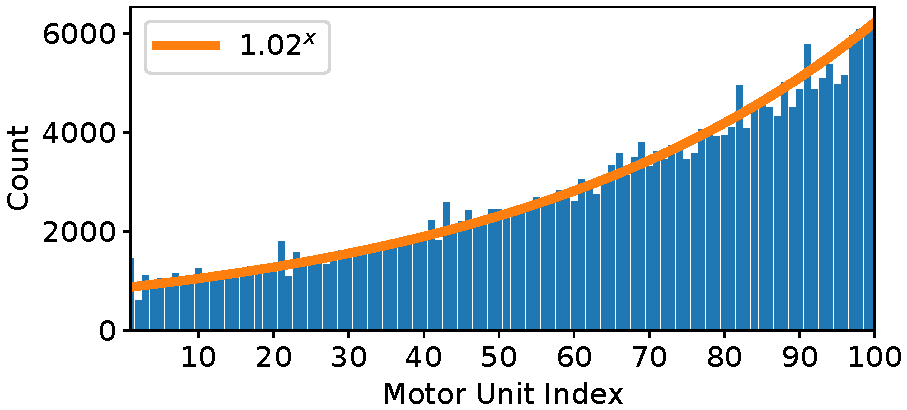
\includegraphics[width=\textwidth]{images/results/application/MU_fibre_distribution_523x523_100mus_txt_fiber_distribution.pdf}%
    \caption{Size distribution for $523\times 523 = \num{273529}$ fibers.}%
    \label{fig:mus_523}%
  \end{subfigure}   
  \caption{Fiber based EMG simulation for the upper arm (biceps) model; Distribution of the sizes of the 100 MUs in the scenarios with different number of fibers.}%
  \label{fig:mu_sizes_100mus}%
\end{figure}%


For every fiber, the algorithm assigns a MU with a close center point with higher probability than a MU whose center is located further away. The total number of fibers per MU is progressing exponentially for the MUs from 1 to 100. The progression is described by an exponential function with basis $1.02$. \Cref{fig:mu_sizes_100mus} shows the MU size distributions for four scenarios with increasing numbers of fibers from \num{169} to \num{273529}. For 169 fibers in \cref{fig:mus_13}, not all 100 MUs get associated with a fiber. Further, it can be seen that the error of the actual size distribution to the exponential function decreases with increasing number of fibers. For the largest scenario in \cref{fig:mus_523}, the MU sizes range from 602 to 6097 fibers.

The number of approximately $\num{3e6}$ fibers in the largest scenario matches the realistic number in a biceps muscle \cite{MacDougall1984}. The number of MUs can be higher in reality, approximately by a factor of 5 \cite{Feinstein1955,MacIntosh2006}. Thus, the modeled MUs in this scenario can be seen as a combination of multiple real MUs. Especially the smallest MUs, which in reality can consists of only some dozens of fibers, are lumped by the first few MUs in our scenario. We restrict the number of MUs to 100 to be able to simulate the same problem also with smaller resolutions, e.g., with only 169 fibers.

\begin{figure}
  \centering%
  \begin{subfigure}[t]{0.47\textwidth}%
    \centering%
    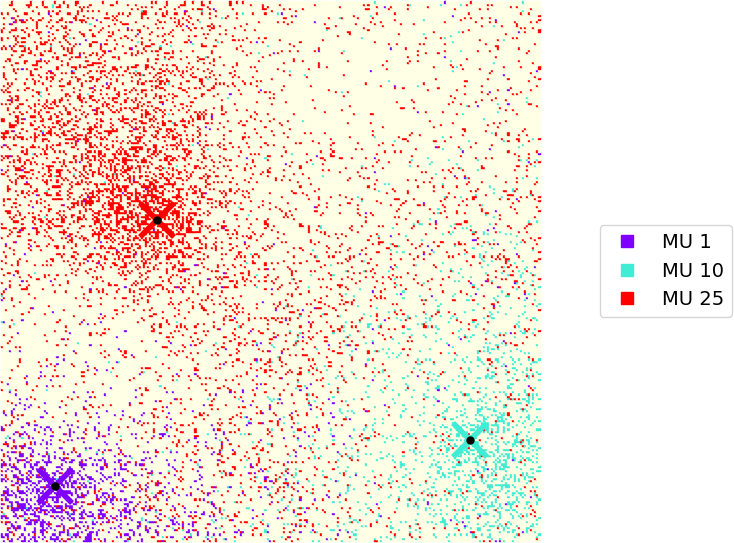
\includegraphics[width=\textwidth]{images/results/application/MU_fibre_distribution_523x523_100mus_txt_0_2d_fiber_distribution_.png}%
    \caption{Partial problem with a quarter of the whole set of fibers and 25 MUs, which occurs in the algorithm 1a described in \cref{sec:muscle_fibers_and_motor_units}. Only three MUs are shown. The MU territory centers are indicated by crosses.}%
    \label{fig:mu_assignment_part0}%
  \end{subfigure} \quad
  \begin{subfigure}[t]{0.47\textwidth}%
    \centering%
    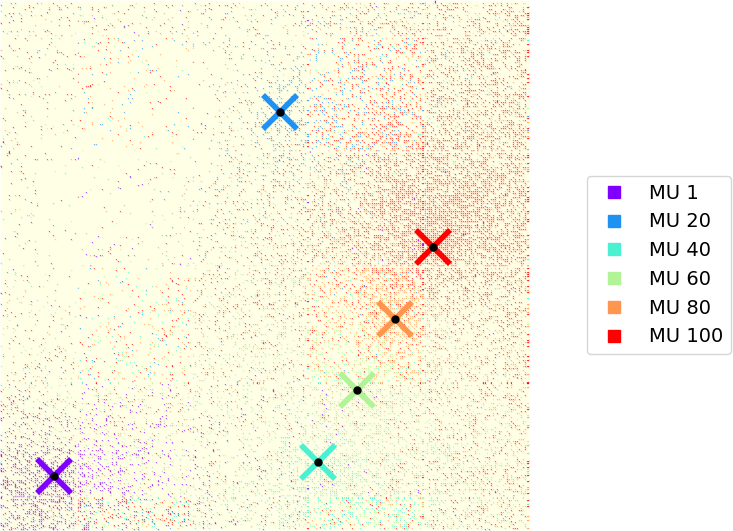
\includegraphics[width=\textwidth]{images/results/application/MU_fibre_distribution_523x523_100mus_txt_2d_fiber_distribution_.png}%
    \caption{The resulting assignments of MUs to fibers after four parts similar to (a) have been combined, here only shown for six MUs.}%
    \label{fig:mu_assignment_total}%
  \end{subfigure} 
  \caption{Fiber based EMG simulation for the upper arm (biceps) model; association of MUs to the fibers. The square domain corresponds to a cross-section in the muscle, every colored point is one fiber, and the color corresponds to the MU. }%
  \label{fig:mu_assignment_100}%
\end{figure}%

As described in \cref{sec:muscle_fibers_and_motor_units}, the MU assignment algorithm ensures that neighboring fibers are part of different MUs, by splitting the assignment problem for the given set of fibers into four smaller problems and then interleaving the results of the four parts. \Cref{fig:mu_assignment_part0} shows the first of these four parts, where 25 MUs are associated to a subset of the fibers for the largest scenario with \num{273529} fibers. It can be seen that the three visualized MUs are largely clustered around their MU territory centers.

The final association of fibers and MUs is given in \cref{fig:mu_assignment_total}. Six selected MUs are shown, of which the first, MU 1, corresponds to the first MU in \cref{fig:mu_assignment_part0}. The figure shows that the fibers, especially the ones of the larger MUs, are distributed far across the muscle. Comparing the smallest MU, MU 1, with the largest MU, MU 100, gives an impression of the MU size differences in this scenario.


\begin{table}
  \centering%
  \begin{tabular}{|r|c|c|c|r|r|c|c|}
    \hline
    \#fibers        & \multicolumn{2}{c|}{3D stride} & 2D surface  & 3D dofs    & 0D dofs & \#proc. & \#comp.\\
    \cline{2-3}
                         & $x,y$ & $z$                & mesh       & (k=1000)      &  && nodes\\
    \hline
    $37^2=\num{1369}$    & 2     & 8  & $19 \times 186$  & \num{67}\,k     & \num{8109}\,k  & \num{144} & 3\\[2mm]  % 6x6x4
    $67^2=\num{4489}$    & 2     & 4  & $34 \times 371$  & \num{428}\,k     & \num{26592}\,k  & \num{448} & 7\\[2mm]  % 7x8x8
    $109^2=\num{11881}$  & 2     & 3  & $55 \times 495$  & \num{1497}\,k     & \num{70383}\,k  & \num{1152} & 18\\[2mm]  % 12x12x8
    $187^2=\num{34969}$  & 2     & 2  & $94 \times 741$  & \num{6547}\,k     & \num{207156}\,k  & \num{3600} & 57\\[2mm] % 15x15x16
    $277^2=\num{76729}$  & 2     & 1  & $139 \times 1481$  & \num{28614}\,k  & \num{454542}\,k  & \num{7744} & 121\\[2mm] % 22x22x16
    $523^2=\num{273529}$ & 2     & 1  & $262 \times 1481$  & \num{101661}\,k  & \num{1620}\,M  & \num{26912} & 421\\ % 29x29x32
    \hline
  \end{tabular}
  \caption{Fiber based EMG simulation for the upper arm (biceps) model; Parameters of spatial discretization and parallel partitioning. The 3D stride refers to the stride with which the 3D mesh is generated from the 0D points. The 2D surface is the output of the EMG and corresponds to one face of the 3D mesh.}%
  \label{tab:emg_study_parameters}%
\end{table}

The numeric parameters of the simulations are the same as in the last section. The scenario is computed for a simulation time span of $\SI{1}{\s}$. The MUs are activated in a ramp every $\SI{2}{\ms}$ such that all MUs are active after $\SI{200}{\ms}$. The fiber radius
and the stimulation frequency for the MUs are exponentially distributed with basis $1.02$, similar to the MU size. The fiber radius increases from \SI{40}{\micro\meter} to \SI{55}{\micro\meter}, and the stimulation frequency decreases from \SI{24}{\hertz} to \SI{7}{\hertz} for MUs 1 to 100. A random frequency jitter of \SI{10}{\percent} is assumed.

The surface to volume ratio $A_m$ of the membrane is determined by assuming a cylindrical shape and can be computed from the fiber radius $r$ as $A_m = 2/r$ \cite{Klotz2020}. We model \SI{70}{\percent} slow twitch and \SI{30}{\percent} fast twitch fibers. Accordingly, the membrane capacitance $C_m$ is set to $C_m = \SI{0.58}{\micro\farad\per\centi\meter\squared}$ for the 70 smallest MUs and to $C_m = \SI{1}{\micro\farad\per\centi\meter\squared}$ for the 30 largest MUs.

\Cref{tab:emg_study_parameters} lists the spatial discretization and parallel partitioning parameters. The first column shows the number of fibers. Their number increases, however, the mesh resolution of every 1D fiber mesh stays constant at 1480 elements per fiber. The stride that defines the 3D mesh is given in the second and third columns. The stride in radial direction of the muscle, i.e., in the $x$ and $y$ coordinate directions, stays constant. Because the fiber density increases, the 3D mesh is refined accordingly. The stride along the fibers, i.e., in $z$ direction is reduced, such that the mesh widths of the 3D mesh in all three coordinate directions remain balanced.

The resulting EMG recordings of each simulation are described by 2D meshes, which contain the values of the 3D muscle meshes without fat layer on the surface at one side of the muscle.  The fourth column in \cref{tab:emg_study_parameters} lists the dimensions of these surface meshes. 

The next two columns list the number of dofs in the 3D mesh and the number of dofs in all fibers. For these scenarios, it is not practical to output the 3D mesh or the 1D fiber meshes in regular time intervals, because this would produce large amounts of data that could hardly be processed. Instead, we only output the 2D surface mesh in the ParaView format every \SI{10}{\milli\second}.

The last two columns in \cref{tab:emg_study_parameters} show the numbers of processes and compute nodes that are used on Hawk. One compute node contains 128 physical cores, four cores share a $\SI{16}{\mebi\byte}$ level three (L3) cache. However, we decide to use only 64 cores per compute node, i.e., two cores per L3 cache, because measurements showed that this reduces the overall computation times more than it increases the runtime due to the decreased parallelism. The total computation time of this scenario with a timespan of $\SI{1}{\s}$ is $\SI{2}{\hour}$ $\SI{20}{\minute}$ for the scenario with \num{76729} fibers and 7744 processes.

\Cref{fig:emg_hpc,fig:emg_hpc2} show the resulting surface EMG signals for different resolutions. The color visualizes the value of the extracellular potential $\phi_e$ according to the shown color bar. Because of sign conventions in the definitions of the electric potentials, the spikes in the EMG signals, which result from the action potentials, are negative.

The resulting electric potential in \cref{fig:emg_hpc} exhibits different regions of higher activation that move over time from the center of the muscle towards its ends. The size of these regions at time ${t=\SI{179.5}{\ms}}$ decreases from \cref{fig:emg37} to \cref{fig:emg187} as the mesh width decreases. 
Dark colored strong signals can be seen, which mainly correspond to fibers that are located directly underneath the shown muscle surface.
Apart from these strong signals, also weaker artifacts occur, which are shown in yellow and orange colors. They result from the superposition of several fibers of the same or different MUs. The number of recognizable weak signals is higher for the simulations with higher numbers of fibers and finer mesh resolution.

The four scenarios in \cref{fig:emg_hpc} share the material parameters, territory centers and relative size distributions of the 100 MU and the activation scheme. However, the location of the neuromuscular junctions is determined randomly and varies between the scenarios. Therefore, the resulting EMG signals are not refined images of each other.  However, a similarity of activated regions on a coarse scale can be observed in all scenarios.

% results for different mesh widths
\begin{figure}
  \centering%
  \begin{subfigure}[t]{0.19\textwidth}%
    \centering%
    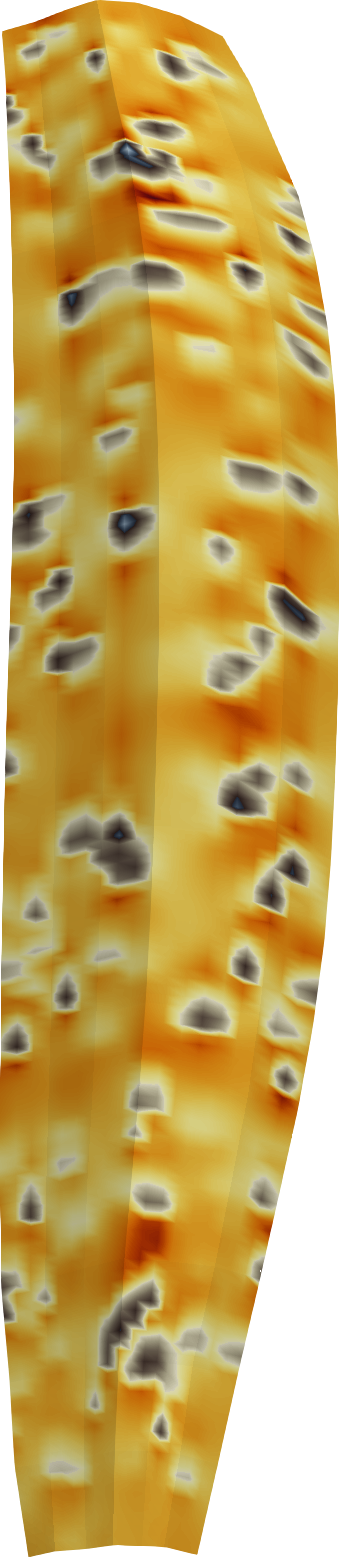
\includegraphics[height=12cm]{images/results/application/emg37.png}%
    \caption{$1369$ fibers.}%
    \label{fig:emg37}%
  \end{subfigure} \,
  \begin{subfigure}[t]{0.19\textwidth}%
    \centering%
    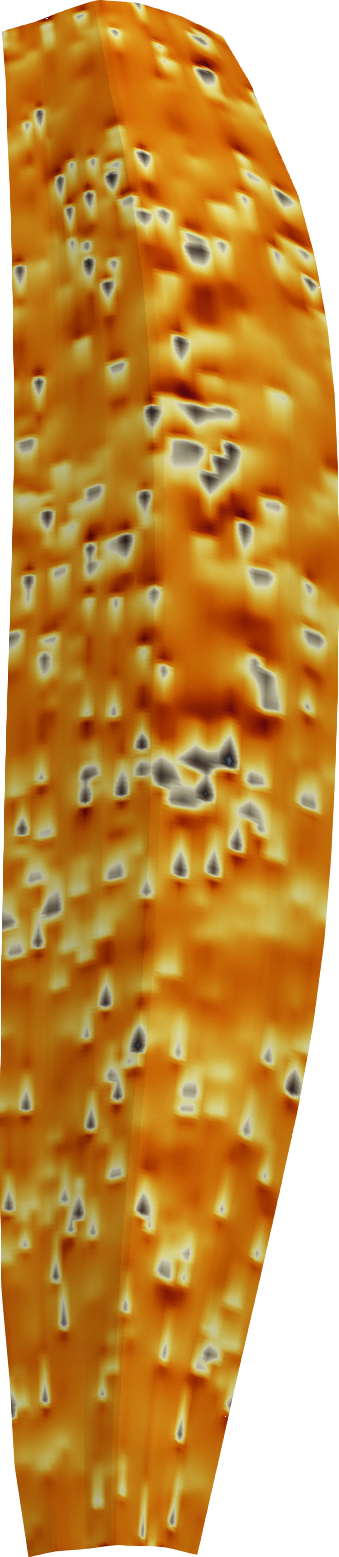
\includegraphics[height=12cm]{images/results/application/emg67.png}%
    \caption{$4489$ fibers.}%
    \label{fig:emg67}%
  \end{subfigure}  \,
  \begin{subfigure}[t]{0.19\textwidth}%
    \centering%
    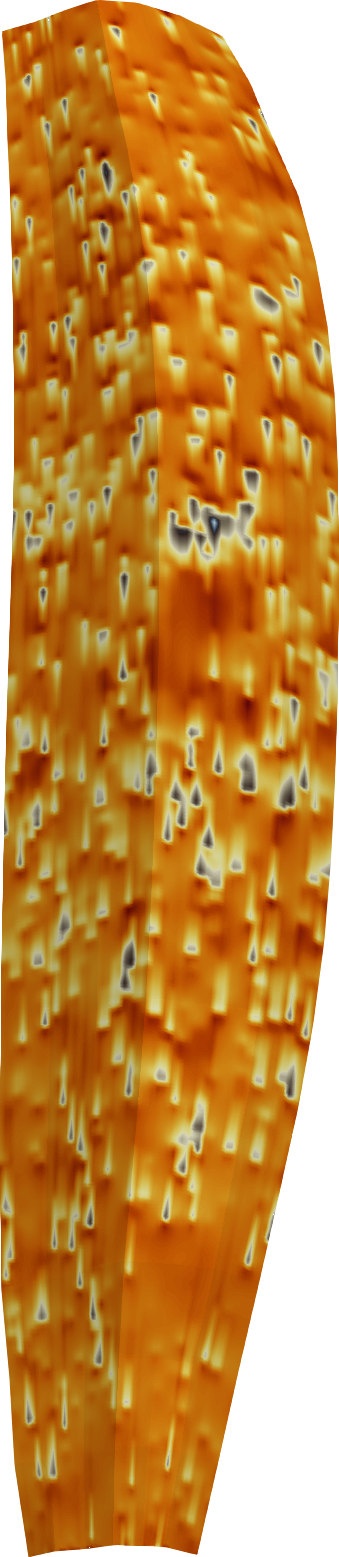
\includegraphics[height=12cm]{images/results/application/emg109.png}%
    \caption{$\num{11881}$ fibers.}%
    \label{fig:emg109}%
  \end{subfigure}    \,
  \begin{subfigure}[t]{0.35\textwidth}%
    \centering%
    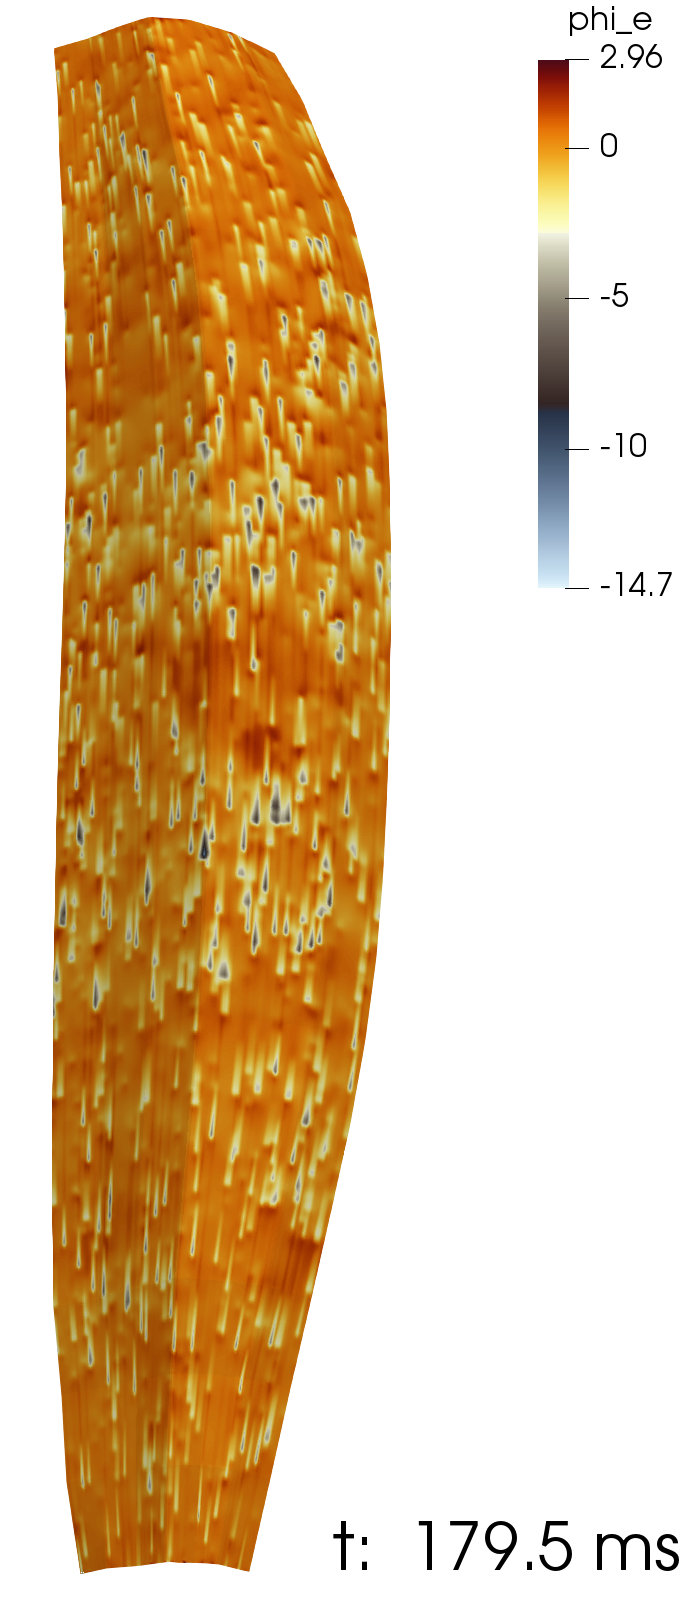
\includegraphics[height=12cm]{images/results/application/emg187.png}%
    \caption{$\num{34969}$ fibers.}%
    \label{fig:emg187}%
  \end{subfigure}   
  \caption{Fiber based EMG simulation for the upper arm (biceps) model; simulated surface EMG signals for different numbers of fibers and different mesh widths of the 3D mesh, see \cref{tab:emg_study_parameters} for details. The same color coding of the EMG signal $\phi_e$ is used in the four scenarios.}%
  \label{fig:emg_hpc}%
\end{figure}%

\Cref{fig:emg_hpc2} shows two more scenarios with a large number of fibers at times of $t\approx \SI{1}{\s}$ and $t\approx \SI{0.4}{\s}$. The scenario in \cref{fig:emg277} simulates approximately \num{76e3} fibers, which is in the order of a third of the realistic number of fibers in the biceps muscle. 
This scenario can also be interpreted as only activating a third of the available fibers in the muscle, resulting in the respective lower percentage of maximum voluntary contraction force.

\Cref{fig:emg273529b} shows the scenario where a realistic number of \num{273e3} fibers was simulated. The computational effort for these two scenarios can only be tackled with High Performance Computing. The last two rows of \cref{tab:emg_study_parameters} show that 121 and 421, repectively, compute nodes were used for the computations.

\Cref{fig:emg273529c,fig:emg273529d} present details of the simulated surface EMG of the scenario in \cref{fig:emg273529b}. The cut outs are indicated by the red boxes in \cref{fig:emg273529b,fig:emg273529c}. \Cref{fig:emg273529d} also visualizes the elements of the 2D and 3D meshes. In both scenarios of \cref{fig:emg_hpc2}, the 3D mesh is as finely resolved in $z$ direction (vertical in \cref{fig:emg273529d}) as the muscle fibers. In transversal direction (horizontal in \cref{fig:emg273529d}), the element sizes are twice as large as the spacing between the fibers. 

The right side of \cref{fig:emg273529d} shows two almost aligned action potentials that propagate towards the top of the image. The upper action potential originates from a fiber that is located at the center between the element boundaries. Its electric potential is distributed to two adjacent nodes on the surface mesh, having the same activated values.
In contrast, the lower action potential results from a fiber that is directly located on the element boundaries. It can be seen that the activation on the surface decays rapidly in transverse (horizontal) direction, as the neighbor elements already almost exhibit the same electric potential as the background level. This underlines the importance to use finely resolved meshes to accurately represent surface EMG signals.


% results for different mesh widths
\begin{figure}
  %\centering%
  \begin{subfigure}{0.30\textwidth}%
    \centering%
    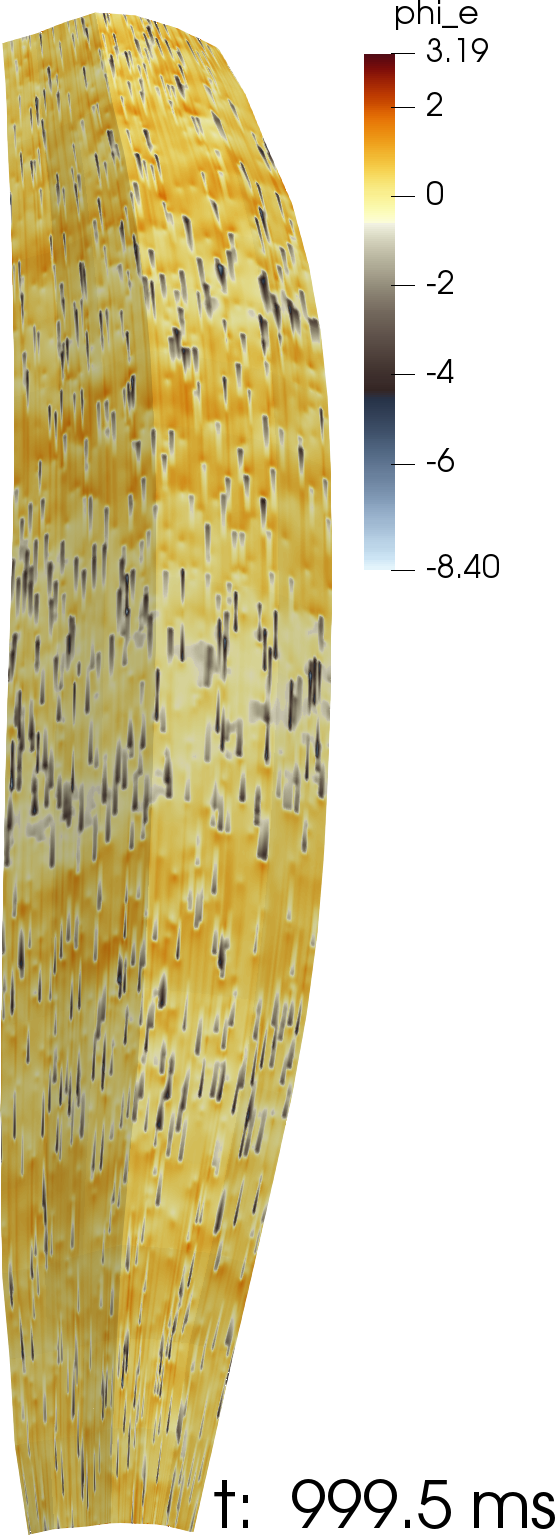
\includegraphics[height=125mm]{images/results/application/emg277.png}%
    \caption{\num{76729} fibers.}%
    \label{fig:emg277}%
  \end{subfigure}\,
  \begin{subfigure}{0.30\textwidth}%
    \centering%
    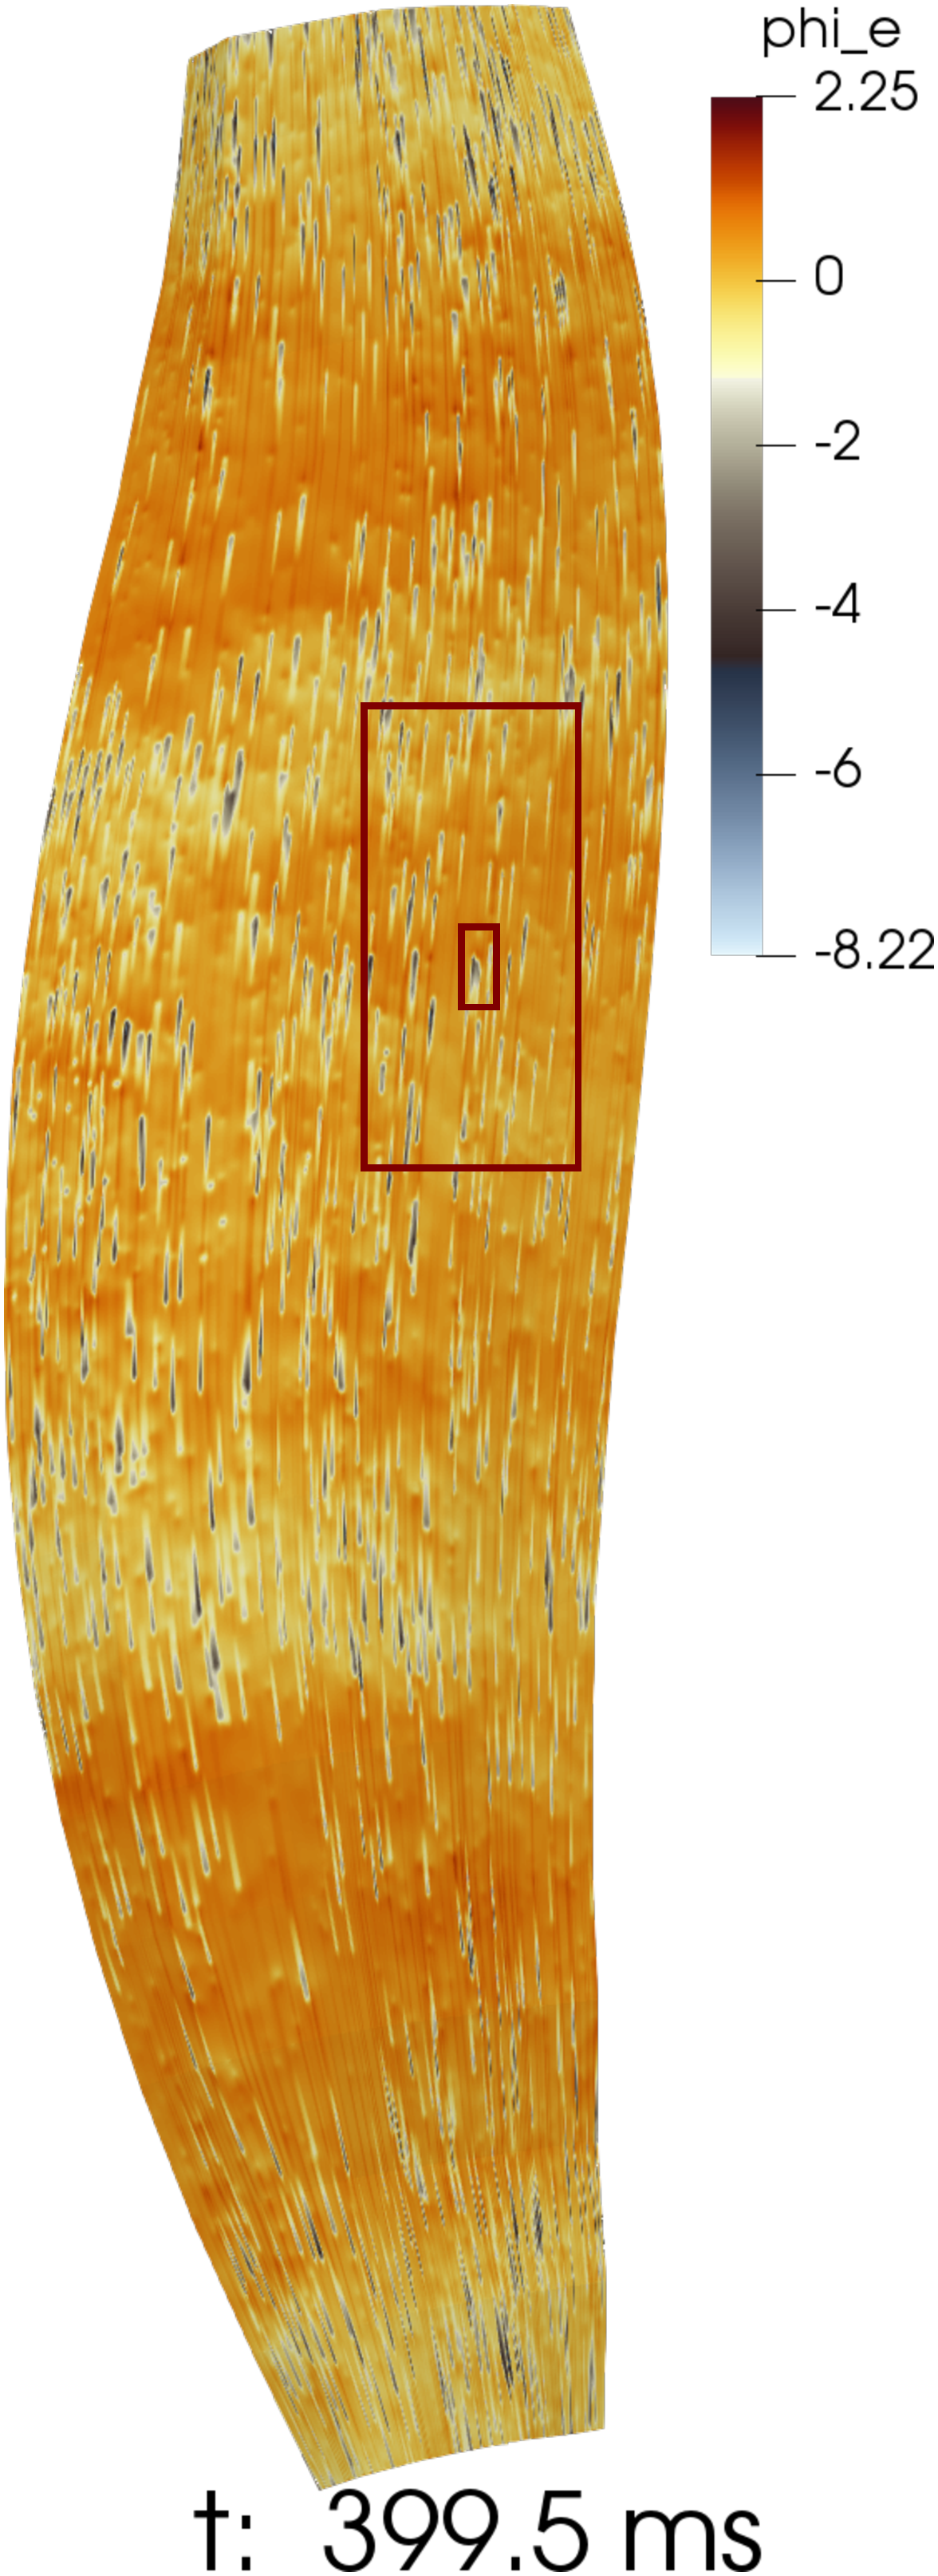
\includegraphics[height=125mm]{images/results/application/emg523.pdf}%
    \caption{\num{273529} fibers.}%
    \label{fig:emg273529b}%
  \end{subfigure}\hspace{-1cm}
  \begin{minipage}{0.5\textwidth}
    \vspace{48mm}
    \begin{subfigure}[t]{0.5\textwidth}%
      \centering%
      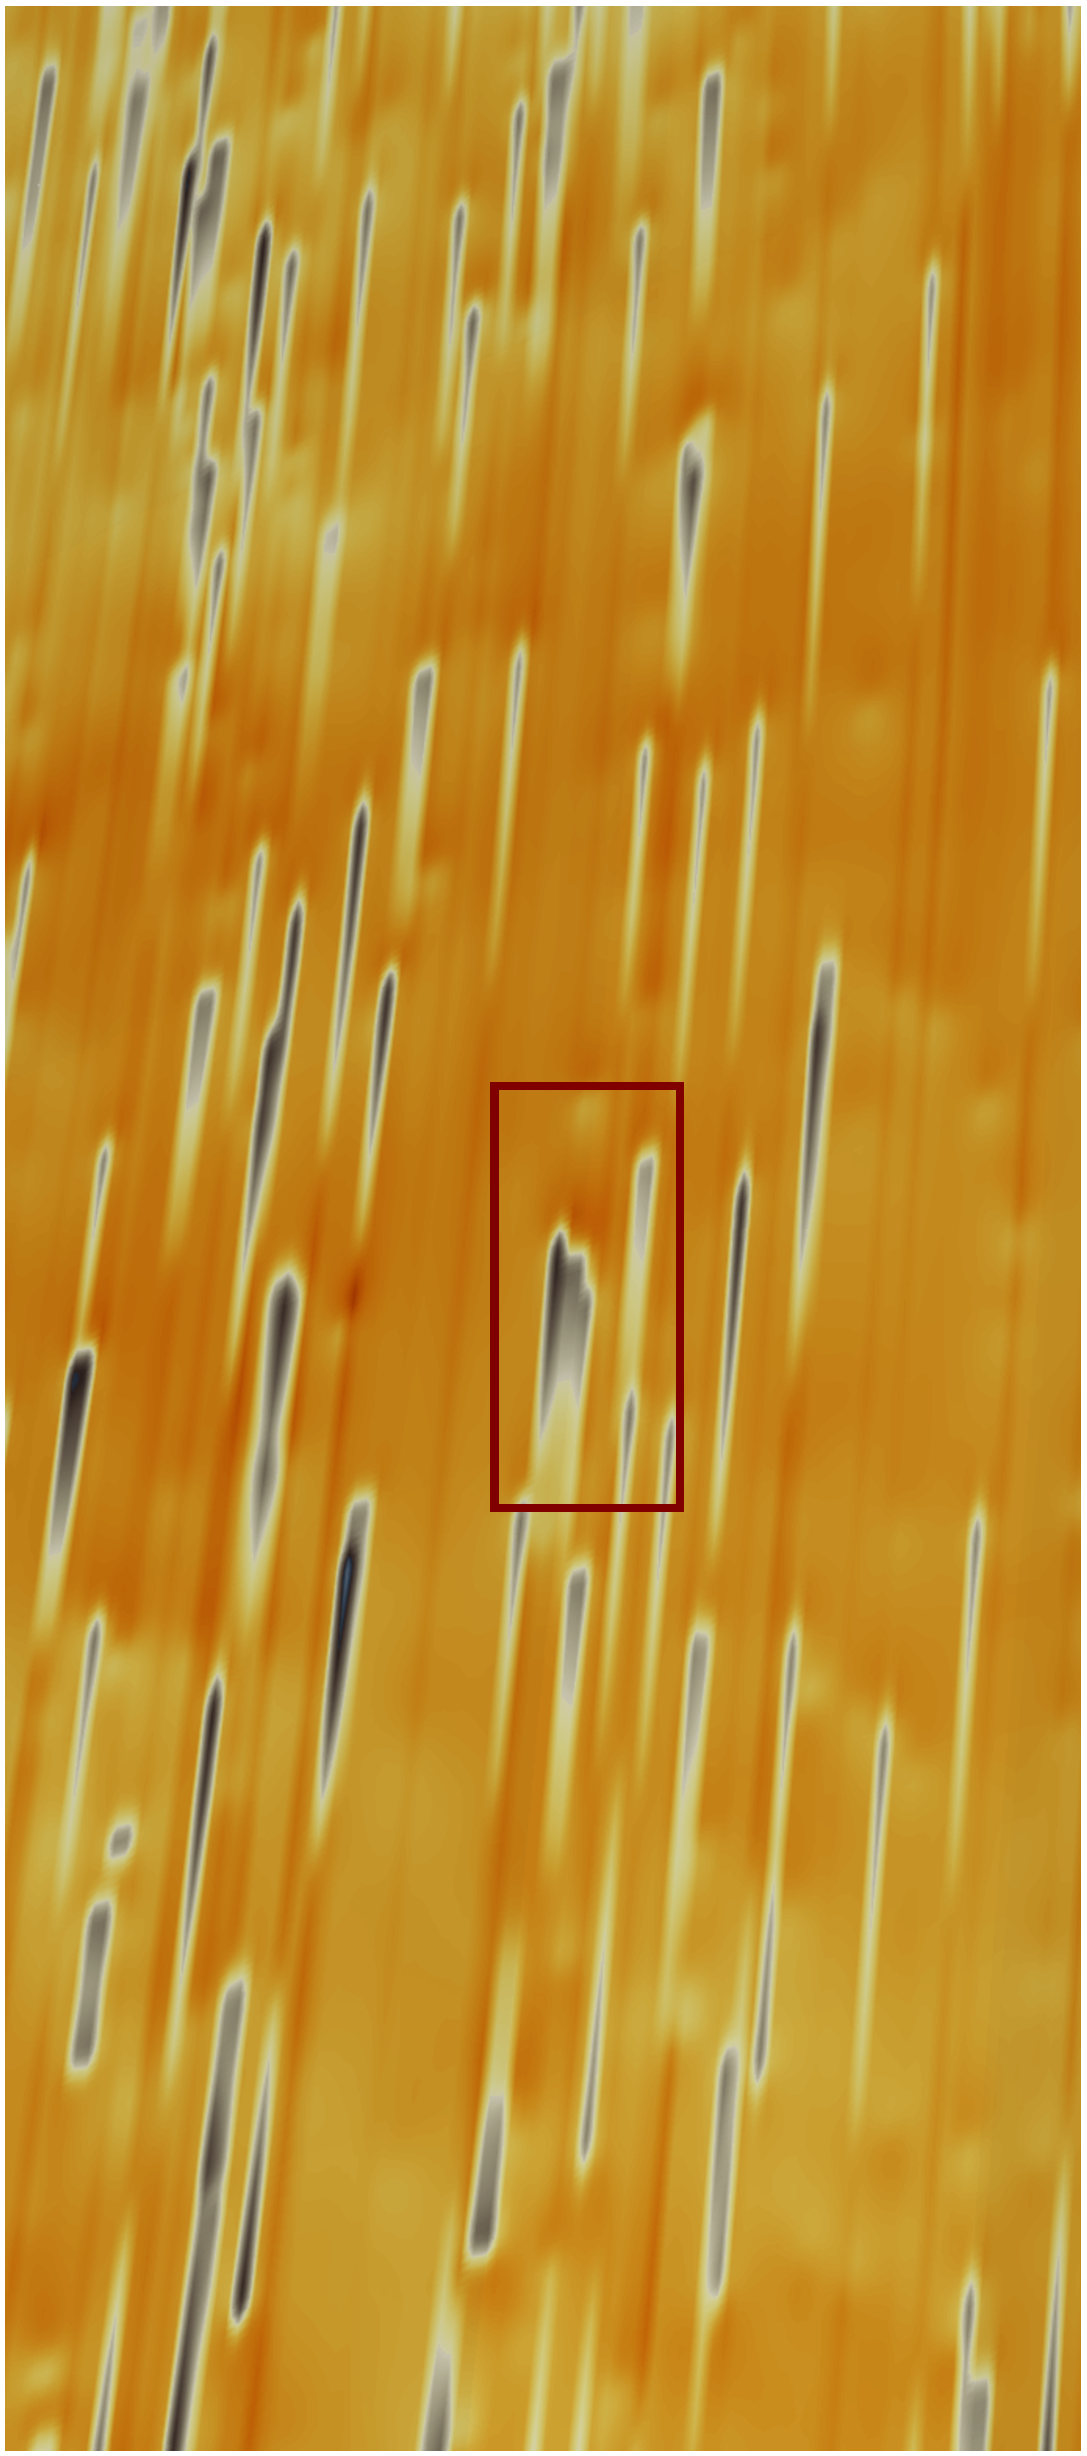
\includegraphics[height=77mm]{images/results/application/emg523-1.pdf}%
      \caption{Detail view.}%
      \label{fig:emg273529c}%
    \end{subfigure}\hspace{-5mm}
    \begin{subfigure}[t]{0.49\textwidth}%
      \centering%
      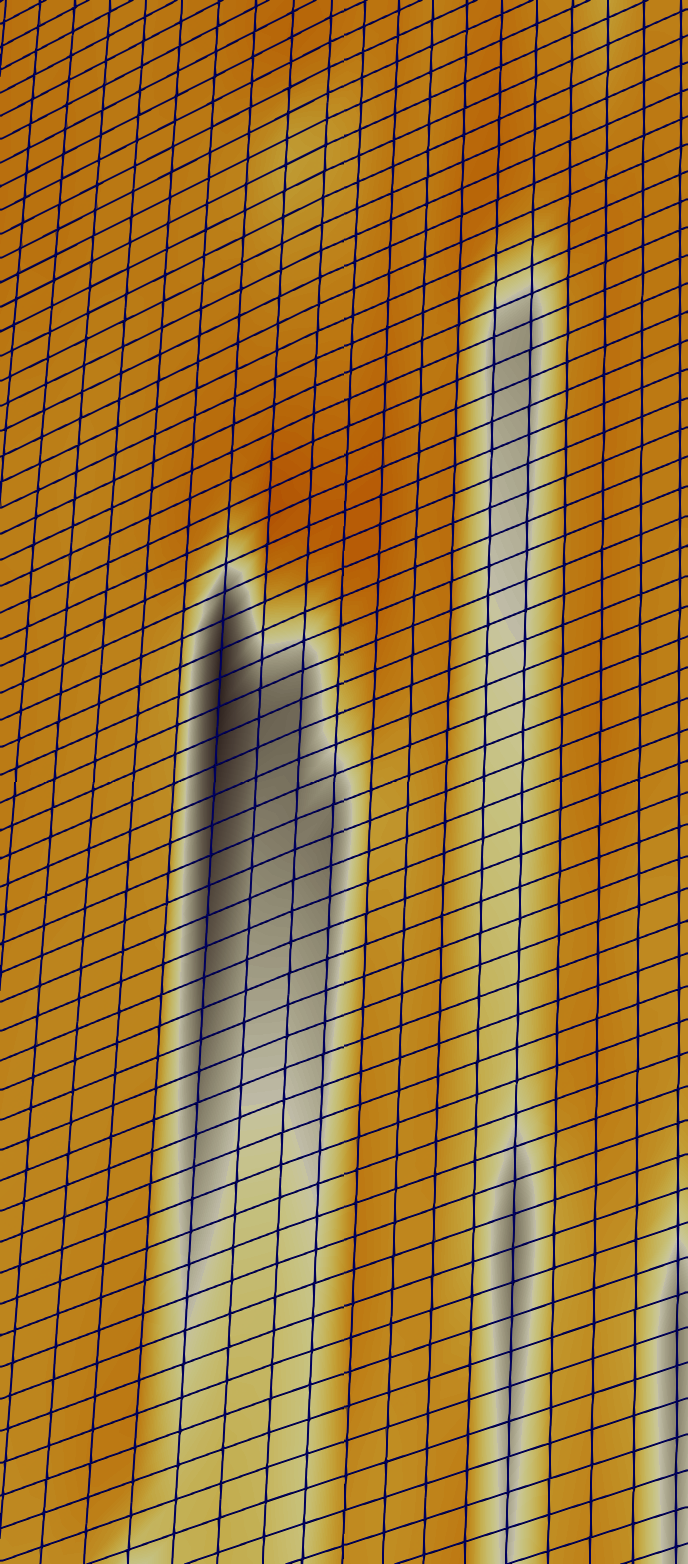
\includegraphics[height=77mm]{images/results/application/emg523-2.png}%
      \caption{Detail view.}%
      \label{fig:emg273529d}%
    \end{subfigure}
  \end{minipage}
  \caption{Fiber based EMG simulation for the upper arm (biceps) model; simulated surface EMG signals with realistic fiber counts, continued from \cref{fig:emg_hpc}. Figure (a) shows a scenario with \num{76729} fibers, which is approximately a third of the realistic number for the biceps muscle. Figures (b)-(d) show the result with a realistic number of \num{273529} fibers. (c) shows a detail view of (b) indicated by the outer red box. (d) shows another zoomed in view of (b) and (c), also indicated by the red boxes.}%
  \label{fig:emg_hpc2}%
\end{figure}%

% single figure of the largest scenario, also with mesh width shown
% 2d fiber distribution for the largest scenario that was run

%partitioning  2* 2* 1=    4    7^2=    49 fibers, fibers/rank: 12.250000, need    1 nodes
%partitioning  3* 3* 2=   18   13^2=   169 fibers, fibers/rank: 9.388889, need    1 nodes
%partitioning  4* 4* 4=   64   25^2=   625 fibers, fibers/rank: 9.765625, need    1 nodes
%partitioning  6* 6* 4=  144   37^2=  1369 fibers, fibers/rank: 9.506944, need    3 nodes
%partitioning  7* 8* 8=  448   67^2=  4489 fibers, fibers/rank: 10.020089, need    7 nodes
%partitioning 12*12* 8= 1152  109^2= 11881 fibers, fibers/rank: 10.313368, need   18 nodes
%partitioning 15*15*16= 3600  187^2= 34969 fibers, fibers/rank: 9.713611, need   57 nodes
%partitioning 22*22*16= 7744  277^2= 76729 fibers, fibers/rank: 9.908187, need  121 nodes
%partitioning 24*24*32=18432  427^2=182329 fibers, fibers/rank: 9.891981, need  288 nodes
%partitioning 29*29*32=26912  523^2=273529 fibers, fibers/rank: 10.163830, need  421 nodes
%partitioning 40*40*32=51200  523^2=273529 fibers, fibers/rank: 5.342363, need  800 nodes

% still in queue: 22*22*16= 7744  277^2= 76729 fibers on 121 nodes
%                 40*40*32=51200  523^2=273529 fibers, fibers/rank: 5.342363, need  800 nodes
% chained:
%partitioning 24*24*32=18432  427^2=182329 fibers, fibers/rank: 9.891981, need  288 nodes
%partitioning 29*29*32=26912  523^2=273529 fibers, fibers/rank: 10.163830, need  421 nodes


%% ---------------------------- 523 ------------------------------------------
%scenario_name: hawk2_fibers_emg_523,  n_subdomains: 29 29 32,  n_ranks: 26912,  end_time: 1000.0
%dt_0D:           2.5e-03, diffusion_solver_type:      cg
%dt_1D:           6.3e-04, potential_flow_solver_type: gmres, approx. exp.: True
%dt_splitting:    2.5e-03, emg_solver_type:            cg, emg_initial_guess_nonzero: True
%dt_3D:           5.0e-01, paraview_output: True, optimization_type: vc (AoVS)
%output_timestep: 1.0e+00, surface: 1.0e+01, stimulation_frequency: 0.1 1/ms = 100.0 Hz
                          %fast_monodomain_solver_optimizations: True
%fiber_file:              /lustre/cray/ws9/2/ws/icbbnmai-opendihu1/opendihu-hawk-gnu/examples/electrophysiology/input/left_biceps_brachii_523x523fibers.bin
%cellml_file:             /lustre/cray/ws9/2/ws/icbbnmai-opendihu1/opendihu-hawk-gnu/examples/electrophysiology/input/hodgkin_huxley_1952.c
%fiber_distribution_file: /lustre/cray/ws9/2/ws/icbbnmai-opendihu1/performance/opendihu/19_hawk_fibers_emg/fiber_distribution/MU_fibre_distribution_523x523_100mus.txt
%firing_times_file:       /lustre/cray/ws9/2/ws/icbbnmai-opendihu1/opendihu-hawk-gnu/examples/electrophysiology/input/MU_firing_times_always.txt
%********************************************************************************
%prefactor: sigma_eff/(Am*Cm) = 0.0132 = 3.828 / (500.0*0.58)
%diffusion solver type: cg
%n fibers:              273529 (523 x 523), sampled by stride 2 x 2
%n points per fiber:    1481, sampled by stride 1
%26912 ranks, partitioning: x29 x y29 x z32
%523 x 523 = 273529 fibers, per partition: 18 x 18 = 324
%per fiber: 1D mesh    nodes global: 1481, local: 47
  %sampling 3D mesh with stride 2 x 2 x 1 
    %linear 3D mesh    nodes global: 262 x 262 x 1481 = 101661764, local: 9 x 9 x 47 = 3807
    %linear 3D mesh elements global: 261 x 261 x 1480 = 100819080, local: 9 x 9 x 47 = 3807
%number of degrees of freedom:
                    %1D fiber:       1481  (per process: 47)
            %0D-1D monodomain:       5924  (per process: 188)
 %all fibers 0D-1D monodomain: 1620385796  (per process: 60912)
                 %3D bidomain:  101661764  (per process: 3807)
                       %total: 1722047560  (per process: 64719)
%Python config parsed in 35.1s.

%% ---------------------------- 277 ------------------------------------------
%scenario_name: hawk2_fibers_emg_277,  n_subdomains: 22 22 16,  n_ranks: 7744,  end_time: 1000.0
%dt_0D:           2.5e-03, diffusion_solver_type:      cg
%dt_1D:           6.3e-04, potential_flow_solver_type: gmres, approx. exp.: True
%dt_splitting:    2.5e-03, emg_solver_type:            cg, emg_initial_guess_nonzero: True
%dt_3D:           5.0e-01, paraview_output: True, optimization_type: vc (AoVS)
%output_timestep: 1.0e+00, surface: 1.0e+01, stimulation_frequency: 0.1 1/ms = 100.0 Hz
                          %fast_monodomain_solver_optimizations: True
%fiber_file:              /lustre/cray/ws9/2/ws/icbbnmai-opendihu1/opendihu-hawk-gnu/examples/electrophysiology/input/left_biceps_brachii_277x277fibers.bin
%cellml_file:             /lustre/cray/ws9/2/ws/icbbnmai-opendihu1/opendihu-hawk-gnu/examples/electrophysiology/input/hodgkin_huxley_1952.c
%fiber_distribution_file: /lustre/cray/ws9/2/ws/icbbnmai-opendihu1/performance/opendihu/19_hawk_fibers_emg/fiber_distribution/MU_fibre_distribution_277x277_100mus.txt
%firing_times_file:       /lustre/cray/ws9/2/ws/icbbnmai-opendihu1/opendihu-hawk-gnu/examples/electrophysiology/input/MU_firing_times_always.txt
%********************************************************************************
%prefactor: sigma_eff/(Am*Cm) = 0.0132 = 3.828 / (500.0*0.58)
%diffusion solver type: cg
%n fibers:              76729 (277 x 277), sampled by stride 2 x 2
%n points per fiber:    1481, sampled by stride 1
%7744 ranks, partitioning: x22 x y22 x z16
%277 x 277 = 76729 fibers, per partition: 12 x 12 = 144
%per fiber: 1D mesh    nodes global: 1481, local: 93
  %sampling 3D mesh with stride 2 x 2 x 1
    %linear 3D mesh    nodes global: 139 x 139 x 1481 = 28614401, local: 7 x 7 x 93 = 4557
    %linear 3D mesh elements global: 138 x 138 x 1480 = 28185120, local: 7 x 7 x 93 = 4557
%number of degrees of freedom:
                    %1D fiber:       1481  (per process: 93)
            %0D-1D monodomain:       5924  (per process: 372)
 %all fibers 0D-1D monodomain:  454542596  (per process: 53568)
                 %3D bidomain:   28614401  (per process: 4557)
                       %total:  483156997  (per process: 58125)

%% ---------------------------- 187 ------------------------------------------
%scenario_name: hawk2_fibers_emg_187,  n_subdomains: 15 15 16,  n_ranks: 3600,  end_time: 1000.0
%dt_0D:           2.5e-03, diffusion_solver_type:      cg
%dt_1D:           6.3e-04, potential_flow_solver_type: gmres, approx. exp.: True
%dt_splitting:    2.5e-03, emg_solver_type:            cg, emg_initial_guess_nonzero: True
%dt_3D:           5.0e-01, paraview_output: True, optimization_type: vc (AoVS)
%output_timestep: 1.0e+00, surface: 1.0e+01, stimulation_frequency: 0.1 1/ms = 100.0 Hz
%                          fast_monodomain_solver_optimizations: True
%fiber_file:              /lustre/cray/ws9/2/ws/icbbnmai-opendihu1/opendihu-hawk-gnu/examples/electrophysiology/input/left_biceps_brachii_187x187fibers.bin
%cellml_file:             /lustre/cray/ws9/2/ws/icbbnmai-opendihu1/opendihu-hawk-gnu/examples/electrophysiology/input/hodgkin_huxley_1952.c
%fiber_distribution_file: /lustre/cray/ws9/2/ws/icbbnmai-opendihu1/performance/opendihu/19_hawk_fibers_emg/fiber_distribution/MU_fibre_distribution_187x187_100mus.txt
%firing_times_file:       /lustre/cray/ws9/2/ws/icbbnmai-opendihu1/opendihu-hawk-gnu/examples/electrophysiology/input/MU_firing_times_always.txt
%********************************************************************************
%prefactor: sigma_eff/(Am*Cm) = 0.0132 = 3.828 / (500.0*0.58)
%diffusion solver type: cg
%n fibers:              34969 (187 x 187), sampled by stride 2 x 2
%n points per fiber:    1481, sampled by stride 2
%3600 ranks, partitioning: x15 x y15 x z16
%187 x 187 = 34969 fibers, per partition: 12 x 12 = 144
%per fiber: 1D mesh    nodes global: 1481, local: 94
%  sampling 3D mesh with stride 2 x 2 x 2
%    linear 3D mesh    nodes global: 94 x 94 x 741 = 6547476, local: 7 x 7 x 47 = 2303
%    linear 3D mesh elements global: 93 x 93 x 740 = 6400260, local: 7 x 7 x 47 = 2303
%number of degrees of freedom:
%                    1D fiber:       1481  (per process: 94)
%            0D-1D monodomain:       5924  (per process: 376)
% all fibers 0D-1D monodomain:  207156356  (per process: 54144)
%                 3D bidomain:    6547476  (per process: 2303)
%                       total:  213703832  (per process: 56447)
%
%% ---------------------------- 109 ------------------------------------------
%scenario_name: hawk2_fibers_emg_109,  n_subdomains: 12 12 8,  n_ranks: 1152,  end_time: 1000.0
%dt_0D:           2.5e-03, diffusion_solver_type:      cg
%dt_1D:           6.3e-04, potential_flow_solver_type: gmres, approx. exp.: True
%dt_splitting:    2.5e-03, emg_solver_type:            cg, emg_initial_guess_nonzero: True
%dt_3D:           5.0e-01, paraview_output: True, optimization_type: vc (AoVS)
%output_timestep: 1.0e+00, surface: 1.0e+01, stimulation_frequency: 0.1 1/ms = 100.0 Hz
%                          fast_monodomain_solver_optimizations: True
%fiber_file:              /lustre/cray/ws9/2/ws/icbbnmai-opendihu1/opendihu-hawk-gnu/examples/electrophysiology/input/left_biceps_brachii_109x109fibers.bin
%cellml_file:             /lustre/cray/ws9/2/ws/icbbnmai-opendihu1/opendihu-hawk-gnu/examples/electrophysiology/input/hodgkin_huxley_1952.c
%fiber_distribution_file: /lustre/cray/ws9/2/ws/icbbnmai-opendihu1/performance/opendihu/19_hawk_fibers_emg/fiber_distribution/MU_fibre_distribution_109x109_100mus.txt
%firing_times_file:       /lustre/cray/ws9/2/ws/icbbnmai-opendihu1/opendihu-hawk-gnu/examples/electrophysiology/input/MU_firing_times_always.txt
%********************************************************************************
%prefactor: sigma_eff/(Am*Cm) = 0.0132 = 3.828 / (500.0*0.58)
%diffusion solver type: cg
%n fibers:              11881 (109 x 109), sampled by stride 2 x 2
%n points per fiber:    1481, sampled by stride 3
%1152 ranks, partitioning: x12 x y12 x z8
%109 x 109 = 11881 fibers, per partition: 8 x 8 = 64
%per fiber: 1D mesh    nodes global: 1481, local: 186
%  sampling 3D mesh with stride 2 x 2 x 3
%    linear 3D mesh    nodes global: 55 x 55 x 495 = 1497375, local: 5 x 5 x 62 = 1550
%    linear 3D mesh elements global: 54 x 54 x 494 = 1440504, local: 5 x 5 x 62 = 1550
%number of degrees of freedom:
%                    1D fiber:       1481  (per process: 186)
%            0D-1D monodomain:       5924  (per process: 744)
% all fibers 0D-1D monodomain:   70383044  (per process: 47616)
%                 3D bidomain:    1497375  (per process: 1550)
%                       total:   71880419  (per process: 49166)
%
%% ---------------------------- 67 ------------------------------------------
%scenario_name: hawk2_fibers_emg_67,  n_subdomains: 7 8 8,  n_ranks: 448,  end_time: 1000.0
%dt_0D:           2.5e-03, diffusion_solver_type:      cg
%dt_1D:           6.3e-04, potential_flow_solver_type: gmres, approx. exp.: True
%dt_splitting:    2.5e-03, emg_solver_type:            cg, emg_initial_guess_nonzero: True
%dt_3D:           5.0e-01, paraview_output: True, optimization_type: vc (AoVS)
%output_timestep: 1.0e+00, surface: 1.0e+01, stimulation_frequency: 0.1 1/ms = 100.0 Hz
%                          fast_monodomain_solver_optimizations: True
%fiber_file:              /lustre/cray/ws9/2/ws/icbbnmai-opendihu1/opendihu-hawk-gnu/examples/electrophysiology/input/left_biceps_brachii_67x67fibers.bin
%cellml_file:             /lustre/cray/ws9/2/ws/icbbnmai-opendihu1/opendihu-hawk-gnu/examples/electrophysiology/input/hodgkin_huxley_1952.c
%fiber_distribution_file: /lustre/cray/ws9/2/ws/icbbnmai-opendihu1/performance/opendihu/19_hawk_fibers_emg/fiber_distribution/MU_fibre_distribution_67x67_100mus.txt
%firing_times_file:       /lustre/cray/ws9/2/ws/icbbnmai-opendihu1/opendihu-hawk-gnu/examples/electrophysiology/input/MU_firing_times_always.txt
%********************************************************************************
%prefactor: sigma_eff/(Am*Cm) = 0.0132 = 3.828 / (500.0*0.58)
%diffusion solver type: cg
%n fibers:              4489 (67 x 67), sampled by stride 2 x 2
%n points per fiber:    1481, sampled by stride 4
%448 ranks, partitioning: x7 x y8 x z8
%67 x 67 = 4489 fibers, per partition: 8 x 8 = 64
%per fiber: 1D mesh    nodes global: 1481, local: 188
%  sampling 3D mesh with stride 2 x 2 x 4
%    linear 3D mesh    nodes global: 34 x 34 x 371 = 428876, local: 5 x 5 x 47 = 1175
%    linear 3D mesh elements global: 33 x 33 x 370 = 402930, local: 5 x 5 x 47 = 1175
%number of degrees of freedom:
%                    1D fiber:       1481  (per process: 188)
%            0D-1D monodomain:       5924  (per process: 752)
% all fibers 0D-1D monodomain:   26592836  (per process: 48128)
%                 3D bidomain:     428876  (per process: 1175)
%                       total:   27021712  (per process: 49303)
%                       
%% ---------------------------- 37 ------------------------------------------
%scenario_name: hawk2_fibers_emg_37,  n_subdomains: 6 6 4,  n_ranks: 144,  end_time: 1000.0
%dt_0D:           2.5e-03, diffusion_solver_type:      cg
%dt_1D:           6.3e-04, potential_flow_solver_type: gmres, approx. exp.: True
%dt_splitting:    2.5e-03, emg_solver_type:            cg, emg_initial_guess_nonzero: True
%dt_3D:           5.0e-01, paraview_output: True, optimization_type: vc (AoVS)
%output_timestep: 1.0e+00, surface: 1.0e+01, stimulation_frequency: 0.1 1/ms = 100.0 Hz
%                          fast_monodomain_solver_optimizations: True
%fiber_file:              /lustre/cray/ws9/2/ws/icbbnmai-opendihu1/opendihu-hawk-gnu/examples/electrophysiology/input/left_biceps_brachii_37x37fibers.bin
%cellml_file:             /lustre/cray/ws9/2/ws/icbbnmai-opendihu1/opendihu-hawk-gnu/examples/electrophysiology/input/hodgkin_huxley_1952.c
%fiber_distribution_file: /lustre/cray/ws9/2/ws/icbbnmai-opendihu1/performance/opendihu/19_hawk_fibers_emg/fiber_distribution/MU_fibre_distribution_37x37_100mus.txt
%firing_times_file:       /lustre/cray/ws9/2/ws/icbbnmai-opendihu1/opendihu-hawk-gnu/examples/electrophysiology/input/MU_firing_times_always.txt
%********************************************************************************
%prefactor: sigma_eff/(Am*Cm) = 0.0132 = 3.828 / (500.0*0.58)
%diffusion solver type: cg
%n fibers:              1369 (37 x 37), sampled by stride 2 x 2
%n points per fiber:    1481, sampled by stride 8
%144 ranks, partitioning: x6 x y6 x z4
%37 x 37 = 1369 fibers, per partition: 6 x 6 = 36
%per fiber: 1D mesh    nodes global: 1481, local: 376
%  sampling 3D mesh with stride 2 x 2 x 8
%    linear 3D mesh    nodes global: 19 x 19 x 186 = 67146, local: 3 x 3 x 47 = 423
%    linear 3D mesh elements global: 18 x 18 x 185 = 59940, local: 3 x 3 x 47 = 423
%number of degrees of freedom:
%                    1D fiber:       1481  (per process: 376)
%            0D-1D monodomain:       5924  (per process: 1504)
% all fibers 0D-1D monodomain:    8109956  (per process: 54144)
%                 3D bidomain:      67146  (per process: 423)
%                       total:    8177102  (per process: 54567)
%

\begin{reproduce_no_break}
  Use the following commands to run the EMG simulation of the biceps muscle with fat layer and electrodes:
  \begin{lstlisting}[columns=fullflexible,breaklines=true,postbreak=\mbox{\textcolor{gray}{$\hookrightarrow$}\space}]
    cd $\$$OPENDIHU_HOME/examples/electrophysiology/fibers/fibers_fat_emg/build_release
    mpirun -n 16 fibers_fat_emg ../settings_fibers_fat_emg.py 50mus.py
    cd out/50mus
    plot_emg.py ./electrodes.csv ./stimulation.log 25900 26000    # plot the result, here for time span 25.9s - 26s
  \end{lstlisting}
\end{reproduce_no_break}

\subsection{Simulation of EMG electrodes}\label{sec:simfiber_electrodes}
% fibers_fat_emg with electrodes

While the surface EMG simulation results as presented in the last section in \cref{fig:emg_hpc} are suited for insights into the temporal and spatial variation of the electric potential, real experiments are constraint to capture values at the discrete locations of electrodes.
For some applications such as the evaluation of EMG decomposition algorithms, it is beneficial to obtain simulated values at electrode locations.

One possiblity would be to extract nodal values from the simulated surface meshes to simulate electrodes. However, the distance between the nodes in the mesh is not constant in the whole mesh, whereas EMG electrode arrays have fixed inter electrode spacings. We, therefore, follow a different approach and allow to directly specify a grid of electrodes close to the muscle surface. These points are then mapped onto the surface of the muscle and the respective values are calculated by evaluating the finite element interpolant at the respective locations.

In OpenDiHu, a 2D grid of surface electrodes can be defined in the Python settings file by specifying the grid parameters and inter electrode distances. As a result, the simulation distributes the electrodes to the processes according to the parallel partitioning of the 3D mesh, evaluates the computed EMG values at the respective locations and outputs them in a single text file of comma separated values.

\Cref{fig:fibers_fat_emg2_electrodes} shows simulation results of the fiber based electrophysiology model with 49 fibers, fat layer and an array of $12\times 32$ electrodes. The electrodes are visualized as spheres. The muscle fibers below the fat layer are colored according to the transmembrane voltage $V_m$. Only the upper surface of the fat layer is shown and colored according to the extracellular potential $\phi_e$. The EMG electrodes capture the values of the scalar field $\phi_e$ at their locations. The color coding for the electrodes has a different \emph{EMG} color scale to make the resulting signals more distinguishable. Two activated bands across the muscle surface can be seen, which are also present in the electrode values.

\begin{figure}
  \centering%
  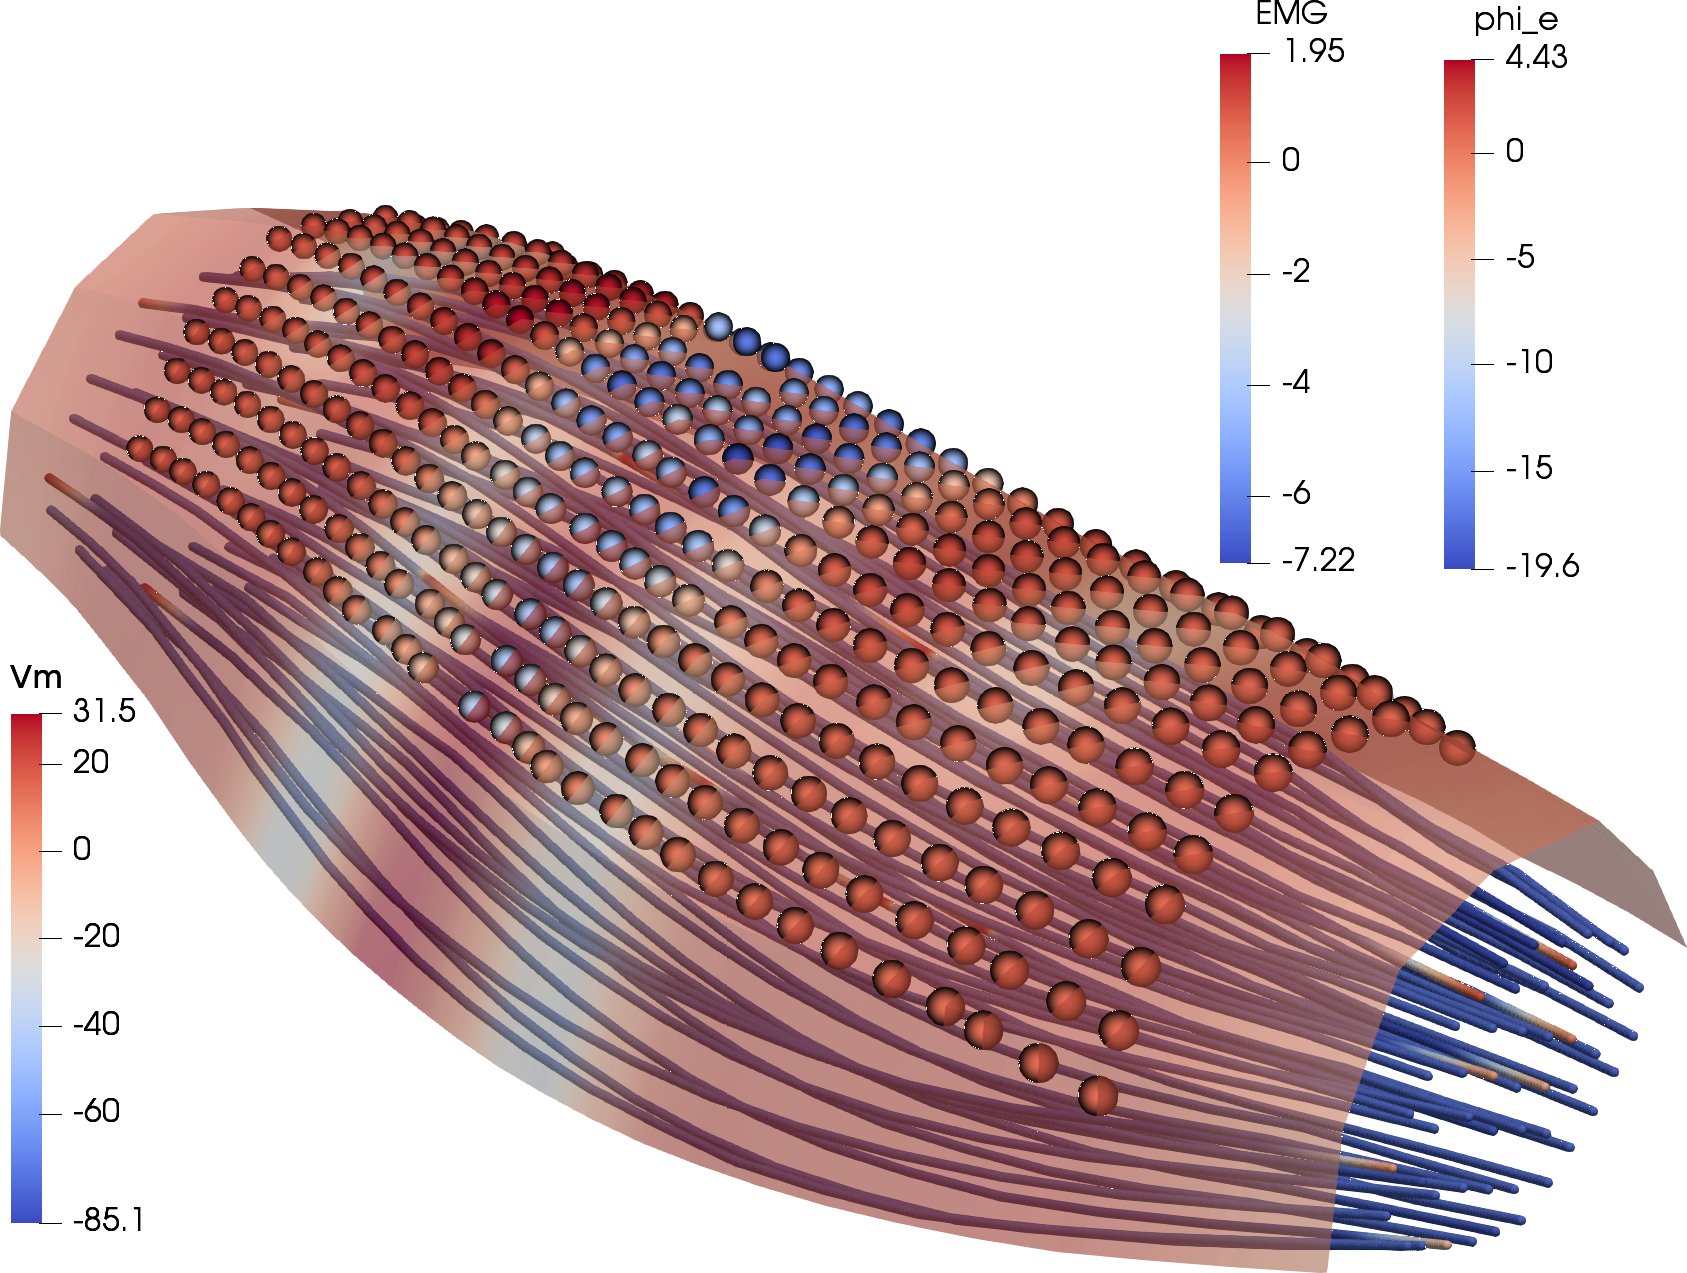
\includegraphics[width=0.7\textwidth]{images/results/application/fibers_fat_emg2.png}%
  \caption{Fiber based EMG simulation for the upper arm (biceps) model; simulation of surface EMG and capturing electrodes. The scenario contains 49 muscle fibers, a fat layer, of which only the surface is shown, and a grid of $12 \times 32$ equidistant electrodes.}%
  \label{fig:fibers_fat_emg2_electrodes}%
\end{figure}

To visually evaluate the simulated EMG signals at the electrodes, OpenDiHu provides utilities to create the visualizations shown in \cref{fig:emg_video}. \Cref{fig:emg_video_37} shows a single frame from an animation. On the upper right, the grid of electrodes is displayed. The EMG signal at the electrodes is given by the colored tiles and changes over time. At the bottom of the image, the activation times of the MUs are visualized. Every horizontal line corresponds to one MU. The colored markers indicate when the respective MU fires. As the shown example visualizes data for \SI{40}{\s}, the individual firing times are not distinguishable. In the animation, a vertical bar moves over the time axis and indicates the current simulation time. The picture displays the EMG values at time $t=\SI{25.975}{\s}$. The upper left of the image shows a text with static information about the dataset, containing the electrode grid size, the inter electrode distance (IED), the end time, the sampling frequency of the electrodes, i.e., the frequency with which the computed EMG signals values are stored to the output file, and the number of MUs.

\Cref{fig:emg_video_plot} shows another, static visualization of simulated EMG data. The diagram contains boxes for all electrodes in the $12\times 32$ grid. The value of the EMG signal is plotted over time in every box for the respective electrode. \Cref{fig:emg_video_plot} visualizes the data of \cref{fig:emg_video_37} for the time interval $[\SI{25.9}{\s},\SI{26}{\s}]$.
The diagram enables experts to visually identify propagating action potentials from the tile columns. The propagation velocity of the action potentials can be estimated from the time shift of matching spikes in vertically adjacent boxes.

\begin{figure}
  \centering%
  \begin{subfigure}[t]{0.6\textwidth}%
    \centering%
    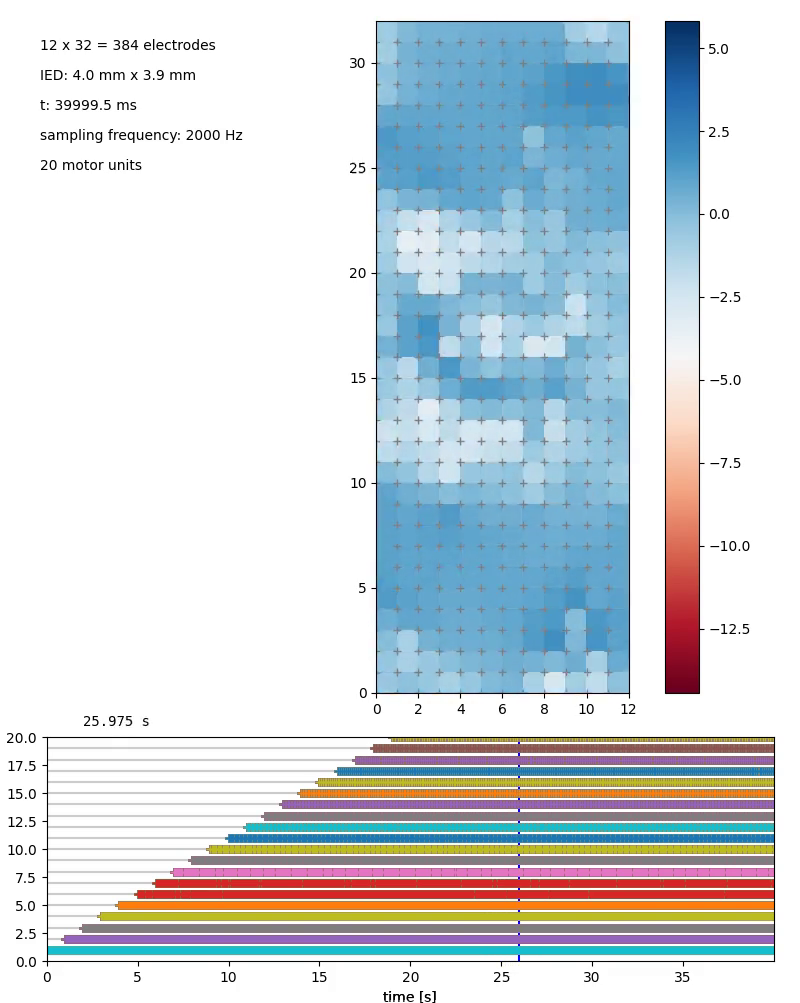
\includegraphics[width=\textwidth]{images/results/application/emg_video_37.png}%
    \caption{Snapshot of an animation of the simulation results that can be generated with the utility of OpenDiHu. The top part visualizes the current values of the EMG electrodes at time $t=\SI{25.975}{\s}$. The bottom part shows the MU activation ramp, each colored line shows to the firing time range of one MU.}%
    \label{fig:emg_video_37}%
  \end{subfigure}  \,
  \begin{subfigure}[t]{0.38\textwidth}%
    \centering%
    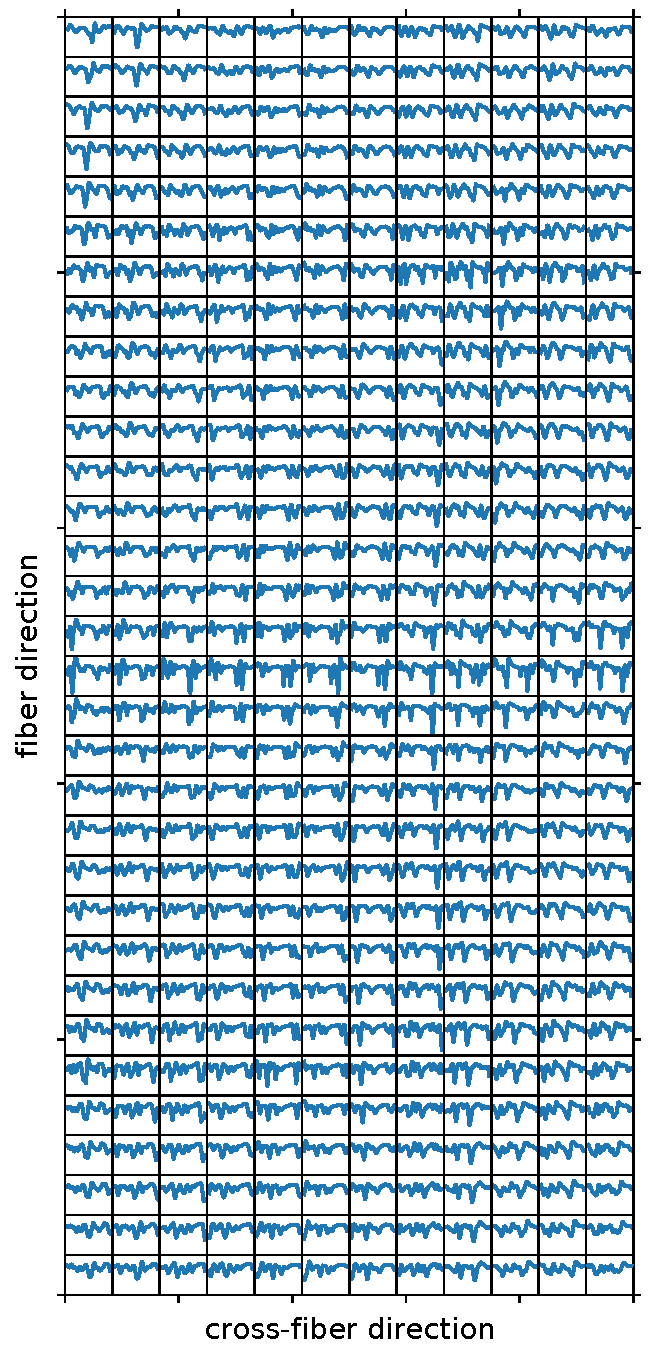
\includegraphics[width=\textwidth]{images/results/application/emg_video_plot.pdf}%
    \caption{Surface EMG at $12 \times 32$ electrodes in the time range $[\SI{25.9}{\s},\SI{26}{\s}]$.}%
    \label{fig:emg_video_plot}%
  \end{subfigure}
  \caption{Fiber based EMG simulation for the upper arm (biceps) model; results of surface EMG obtained at simulated electrodes.}%
  \label{fig:emg_video}%
\end{figure}




\subsection{Decomposition of Surface EMG Signals}\label{sec:simfiber_decomposition}

Surface EMG recordings are a valuable tool to gain insights into the neuromuscular system. They are used, e.g., for the diagnosis of muscular disorders and in clinical studies that aim to advance biomedical understanding.

% why, how are EMG signals generated -> fig
As described earlier, the EMG signals on the skin surface originate from the activated muscle fibers. Effects from volume conduction of action potentials on all muscle fibers are superpositioned and contribute to the EMG signal. The scaling of the contributions to the overall signal depends on several factors such as the distance of the fibers to the skin surface. As all fibers in the same MU get activated simultaneously, each MU`s contribution shows a characteristic \say{shape} in the resulting surface EMG signal. This shape is influenced by the number and location of the muscle fibers relative to the electrodes and the location of the neuromuscular junctions.

In our simulation, the location of the neuromuscular junctions is chosen pseudo-randomly (but deterministic) during initialization in the central \SI{10}{\percent} of every muscle fiber. \Cref{fig:emg_video_37_junctions} shows the state of a simulation with $1369$ fibers at $t=\SI{1}{\ms}$, where all fibers have been activated at $t=\SI{0}{\ms}$. The color coding indicates the potential $V_m$ of the membrane, which at the shown time has only depolarized near the locations of the neuromuscular junctions.

\begin{figure}
  \centering%
  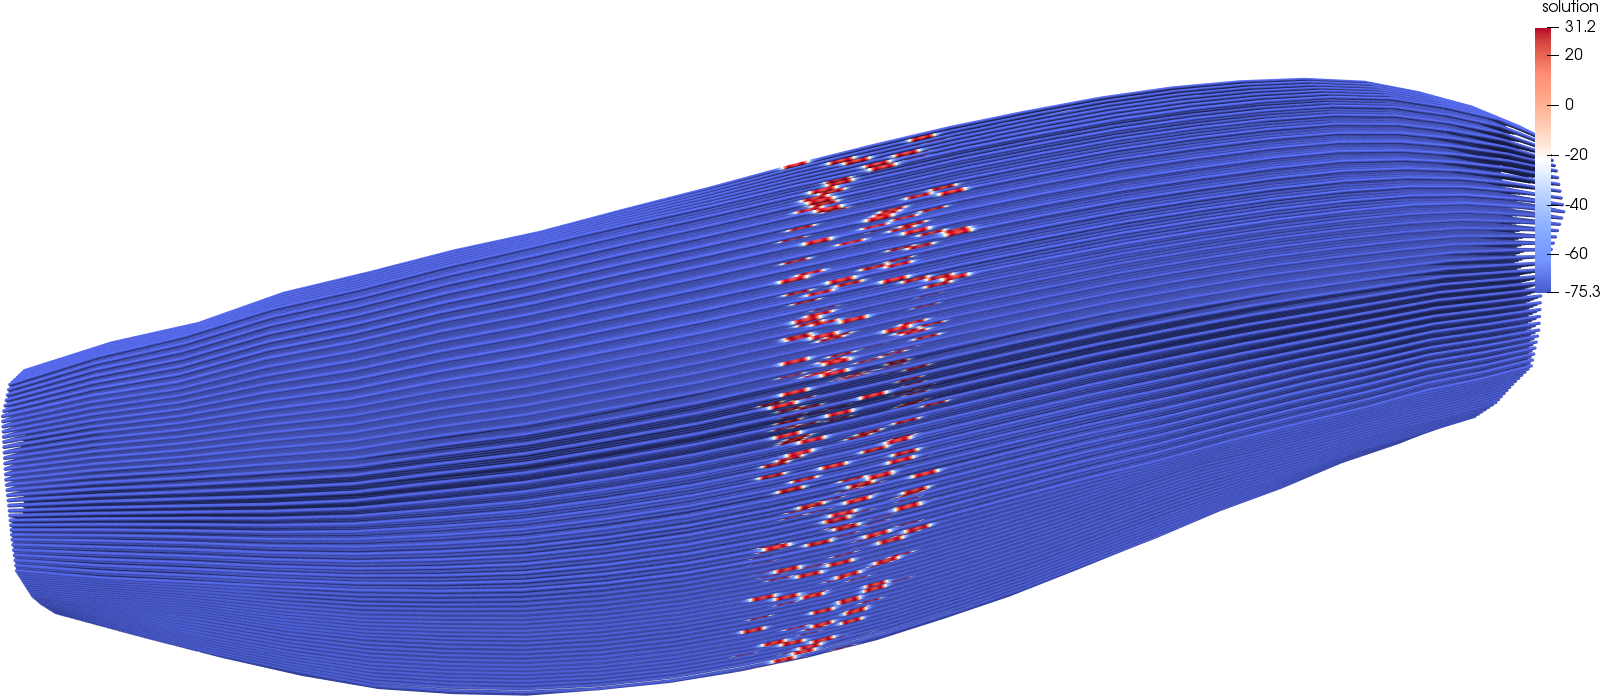
\includegraphics[width=0.85\textwidth]{images/results/application/emg_video_37_junctions.png}%
  \caption{Fiber based EMG simulation for the upper arm (biceps) model; a simulation result that reveals the locations of the neuromuscular junctions. The figure depicts 1369 fibers after $\SI{1}{\ms}$, which have initially been stimulated at the neuromuscular junction. The color coding corresponds to the membrane potential $V_m$, which has a positive value near the points of stimulation.}%
  \label{fig:emg_video_37_junctions}%
\end{figure}

% gCKC method
% Evtl. auch hier in 1-2 Sätzen etwas ausholen, warum man das macht: Die Simulationsdaten enthalten alle Informationen über die tatsächlich dem simulierten EMG-Signal zugrunde liegende Stimulation. Man kann sie also nutzen, um die decomposition methods zu validieren.
Methods exist that seek to decompose the surface EMG signal into the contributions of the individual MUs. Given a surface EMG recording, such methods output a number of recovered MUs and their firing times.
In our simulation studies, all relevant information is available that determines the EMG signal resulting from MU activity: the location of the fibers and their association to MUs, the positions of the neuromuscular junctions and the innervation pulses for each MU.
Thus, our simulation can be used to validate and evaluate EMG decomposition methods.

One popular EMG decomposition method is \emph{Gradient Convolution Kernel Compensation} (gCKC) \cite{Holobar2007b,Holobar2007}, which, in the following, will be outlined and then applied on simulated data.

Most decomposition methods, including the gCKC algorithm, assume that the EMG signal at an electrode is composed of the convolutional mixture of the activity of $N$ MUs.
The activity of each MU $k\in \{1,\dots,N\}$ is described by the innervation pulse trains, which activate the fibers of MU $k$, given as a point process of neural inputs at stimulation times $\varphi_r$. The source signal $s_k$ in the muscle, which represents the effect of MU $k$ is described as a spike $s_k(t) = \sum_r\delta(t - \varphi_r)$, where $\delta$ is the dirac delta function.

The vector of observed EMG value $\bfx \in \R^m$ at a time $t$ is composed of the temporal convolution over $L$ time-shifted sources $\bfs$ and a term $\bfomega$ of additive Gaussion noise:
\begin{align*}
  \bfx(t) = \s{l=0}{L-1}\bfH(l)\,\bfs(t-l) + \bfomega(t).
\end{align*}
Here, $\bfH$ is the $m\times n$ mixing matrix for $m$ observations and $n$ MU sources and $\bfs = (s_k)_{1,\dots,n}$ is the vector of source signals. The sum over $L$ previous values in this convolutive mixture can be reformulated by moving the summation into the matrix-vector product. The dimensions of the matrix $\bfH$ and the vector $\bfs$ are extended accordingly. 
An optimzation problem yields the separation vectors, with which the innervation pulse trains $\varphi_r$ of the MUs can be recovered from the recorded EMG signals $\bfx$. The gCKC algorithm determines the inverse effect of applying the unknown mixing matrix by solving a derived optimization problem using a gradient descent scheme.

The gCKC decomposition algorithm is implemented in the DEMUSE software, a commercial, MATLAB based tool that allows automatic and semi-automatic EMG decomposition \cite{demuse}. In collaboration with Lena Lehmann from the \emph{Institute of Signal Processing and System Theory} and the \emph{Institute for Modelling and Simulation of Biomechanical Systems}, we evaluated the performance of gCKC decomposition on simulated surface EMG signals.

% different performance depending on parameters
We simulate fiber-based electrophysiology scenarios with fat layer and 1369 fibers using the same model parameter as in \cref{sec:effects_of_the_mesh_width_emg}. In the first scenario, a fat layer with thickness of $\SI{1}{\cm}$ is modelled. The simulated EMG signal is sampled in an electrode array with a frequency of $\SI{2}{\kilo\hertz}$ and a grid size of $12 \times 32$ fibers, as shown in \cref{fig:emg_video}.

\Cref{fig:emg_20mus-50s-old2} shows the firing times of the 20 MUs in the first \SI{10}{\second}. The different MUs are initially activated every \SI{100}{\ms} to generate the shown \say{ramp} activation pattern, which later helps to identify the recovered MUs from the decomposition.  From $t=\SI{1.8}{\second}$ on, all MUs fire with their respective constant frequency, subject to jitter values of $\SI{10}{\percent}$.

In this first scenario, the gCKC decomposition algorithm was applied on the first $t=\SI{40}{\second}$ of simulated EMG data. The preconfigured algorithm in DEMUSE was used without manual intervention. While the simulated EMG recording consisted of an electrode grid of $12 \times 32$ fibers, only a rectangular subset of $5\times 13$ channels at the lower center of the grid was used for the decomposition to mimic a realistic electrode array size. 

In reality, some of the recorded channels may measure invalid data due to inappropriate surface contact of the electrodes, noisy signals at the particular measurement location or other experimental difficulties. The DEMUSE tool can automatically detects such channels and discard the corresponding data from the decomposition scheme. Despite our simulation does not contain invalid channels, the DEMUSE software discarded four of the 65 simulated channels.

% old 20MUs scenario
\begin{figure}
  \centering%
  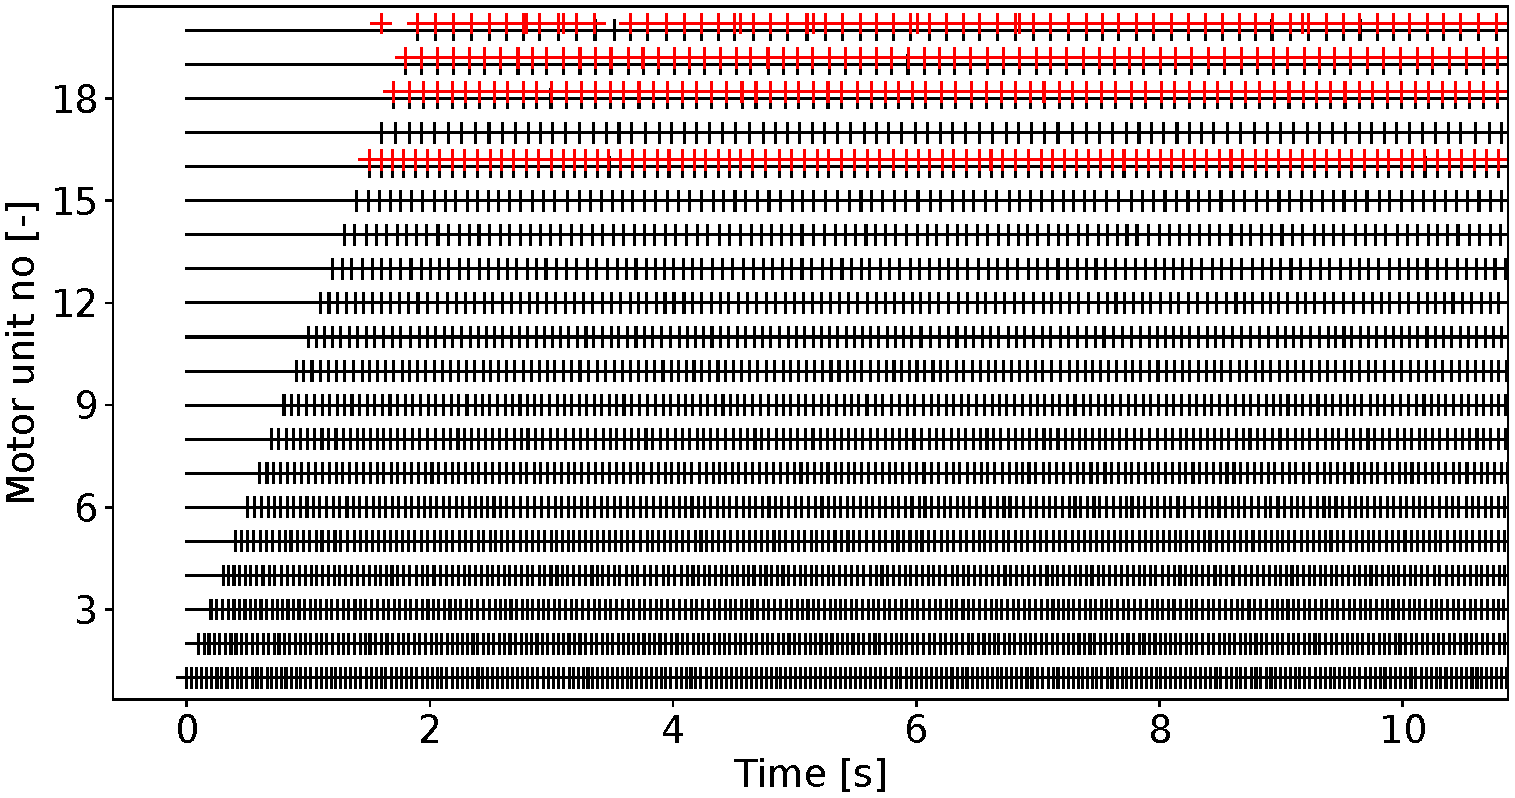
\includegraphics[width=\textwidth]{images/results/application/emg_20mus-50s-old2.pdf}%
  \caption{Validation experiment for EMG decomposition based on fiber-based simulations of the biceps bracchii muscle: Match of EMG decomposition results with simulated data. The true firing pattern over time for the 20 MUs in the simulation is shown by black markers. The recovered firing times of the gradient convolution kernel compensation algorithm are given by the red markers. The algorithm detected the four MUs 16, 18, 19 and 20.}%
  \label{fig:emg_20mus-50s-old2}%
\end{figure}

\Cref{fig:emg_20mus-50s-old2} shows the innervation pulses that were detected by DEMUSE as red vertical markers. A time span of \SI{50}{\s} was simulated of which only the first \SI{11}{\s} are visualized in \cref{fig:emg_20mus-50s-old2}. DEMUSE found four MUs in this scenario, i.e., \SI{20}{\percent} of the 20 simulated MUs. 
The recovered MUs were identified in the set of simulated MUs by matching the  average firing frequency and the activation onset time in the ramp scheme. A first visual comparison with the original stimulation times given by the black markers shows a good agreement.

% old fiber distribution: Smallest MU: 2, Largest MU: 256
\begin{figure}
  \centering%  \,
  \begin{subfigure}[t]{0.45\textwidth}%
    \centering%
    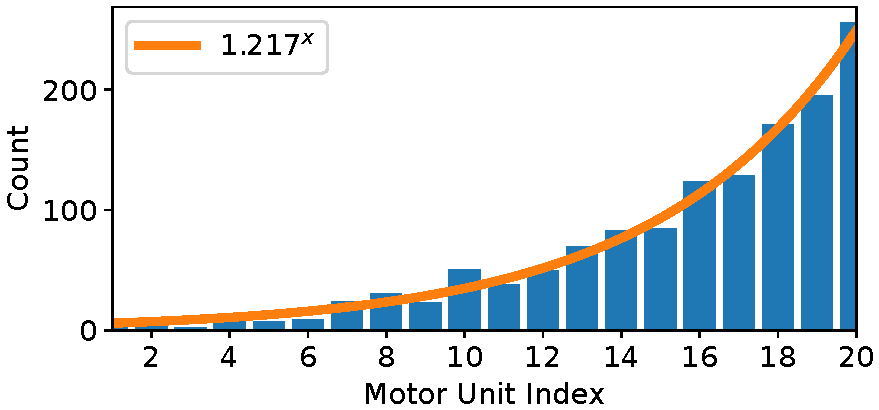
\includegraphics[width=\textwidth]{images/results/application/oldmus2.pdf}%
    \caption{Number of fibers of the 20 MUs in this scenario, following an exponential progression with basis $1.217$.}%
    \label{fig:oldmus_progression}%
  \end{subfigure}\hfill
  \begin{subfigure}[t]{0.45\textwidth}%
    \centering%
    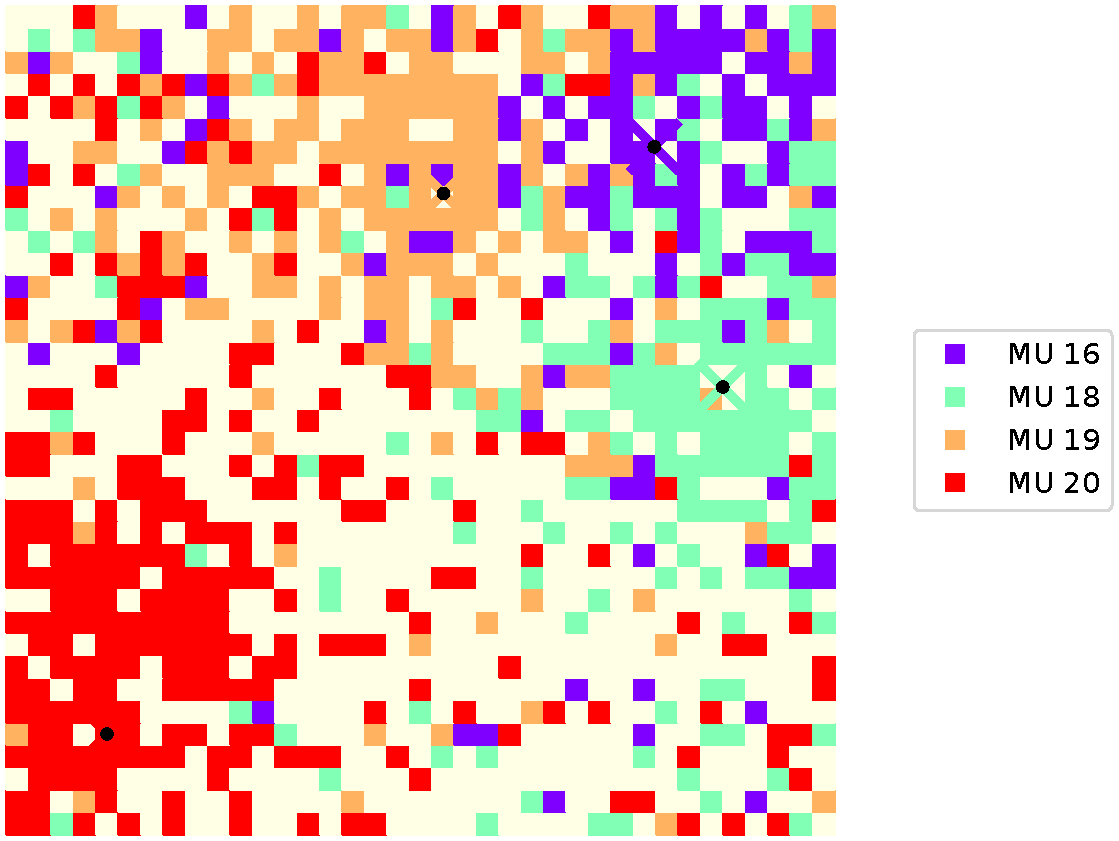
\includegraphics[width=\textwidth]{images/results/application/oldmus1.pdf}%
    \caption{Spatial location of the fibers of the four MUs that were recovered by the EMG decomposition algorithm, indicated by different colors. The territory center points of the MUs used in the generation algorithm are indicated by black dots. The yellow background area corresponds to other MUs, which were not detected.}%
    \label{fig:oldmus_2d}%
  \end{subfigure}
  \caption{Validation experiment for EMG decomposition based on fiber-based simulations of the biceps bracchii muscle: Association of the fibers with motor units for the first scenario with 20 MUs, given in \cref{fig:emg_20mus-50s-old2}.}%
  \label{fig:oldmus}%
\end{figure}

% new fiber distribution: Smallest MU: 42, Largest MU: 102
% number fibers per MU: [ 50  45  43  51  43  42  50  53  61  71  72  69  78  97  87  87 102  74 101  93]
\begin{figure}
  \centering% \,
  \begin{subfigure}[t]{0.45\textwidth}%
    \centering%
    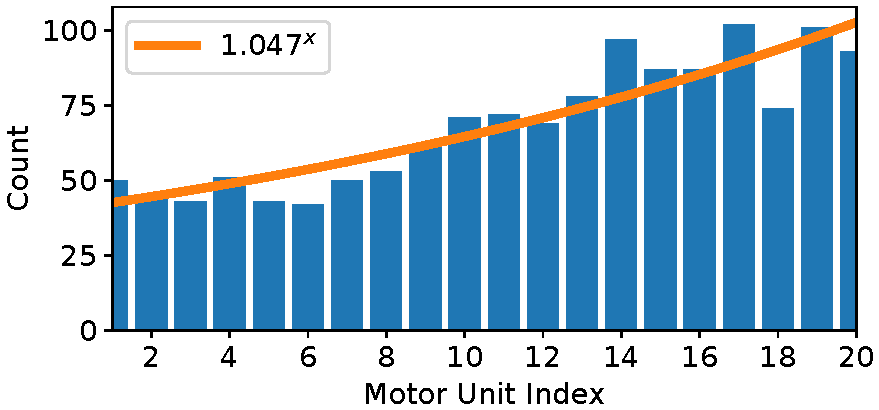
\includegraphics[width=\textwidth]{images/results/application/newmus1.pdf}%
    \caption{Progression of MU sizes. The number of fibers per MU is more balanced in this scenario than in \cref{fig:oldmus_progression}.}%
    \label{fig:newmus_progression}%
  \end{subfigure}\hfill
  \begin{subfigure}[t]{0.45\textwidth}%
    \centering%
    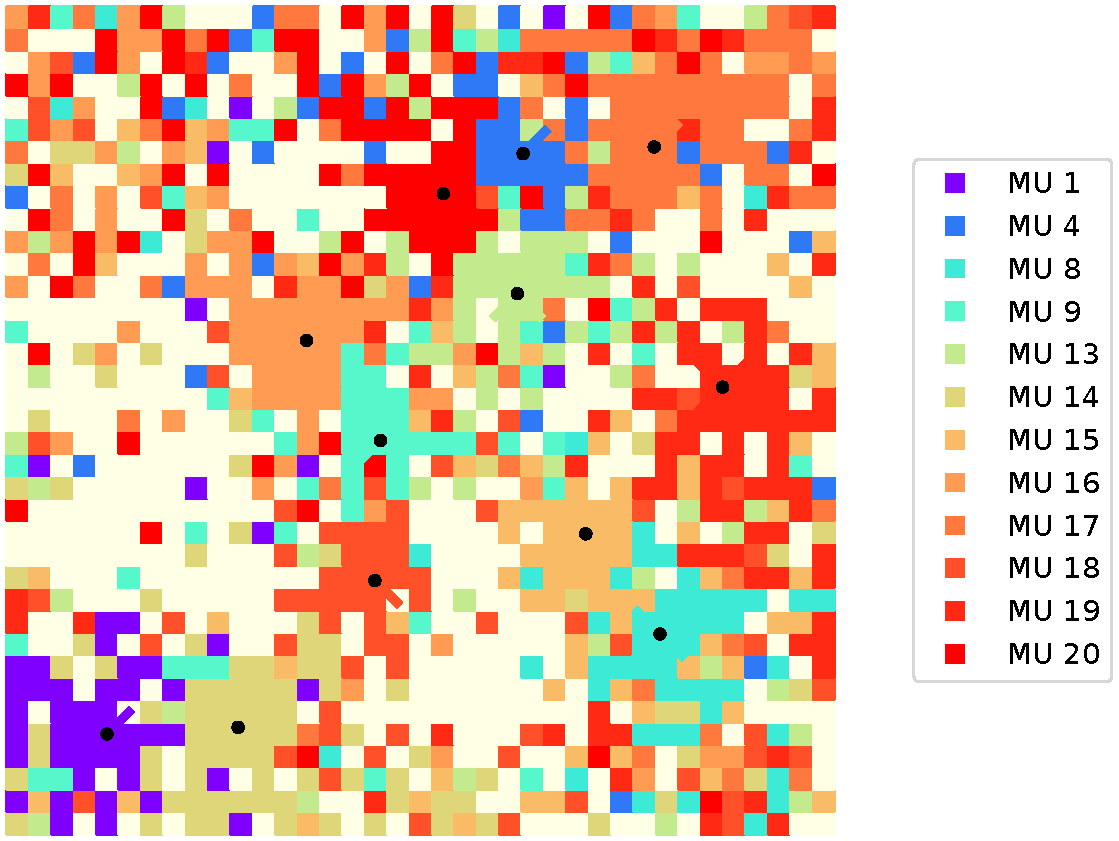
\includegraphics[width=\textwidth]{images/results/application/newmus3.pdf}%
    \caption{Spatial fiber arrangement of the MUs that were detected by the EMG decomposition algorithm, with their center points given by black dots.}%3
    \label{fig:newmus_2d}%
  \end{subfigure} 
  \caption{Validation experiment for EMG decomposition based on fiber-based simulations of the biceps bracchii muscle: Association of the fibers with motor units for the second scenario with 20 MUs, given in \cref{fig:emg_20mus-40s_new}.}%
  \label{fig:newmus}%
\end{figure}

In this scenario, the association of fibers with MUs followed an exponential MU size progression with a basis of approximately $1.2$, as shown in \cref{fig:oldmus_progression}. The smallest MU contained two fibers and the largest MU had 256 fibers. The method 1 described in \cref{sec:method1_assignment} was used to generate the association between fibers and MUs.

\Cref{fig:oldmus_2d} depicts the location of the four MUs that were detected by DEMUSE. The detected MUs have the indices 16, 18, 19 and 20 and correspond to four of the five largest MUs. It can be seen that MUs 18 to 20 are located mainly in the upper half of the muscle cross-section, in proximity to the electrode array at the top of the diagram.
The MU with the most fibers, MU 20, was detected by the decomposition algorithm even though it is located at the lower left of diagram at a large distance to the skin surface.

Two further scenarios were simulated with the same parameters as the first scenario in \cref{fig:emg_20mus-50s-old2}, but instead with 50 and 100 MUs. In these datasets, DEMUSE was able to detect 8 and 12 MUs, which corresponds to \SI{16}{\percent} and \SI{12}{\percent}. 

% new 20MUs scenario
\begin{figure}
  \centering%
  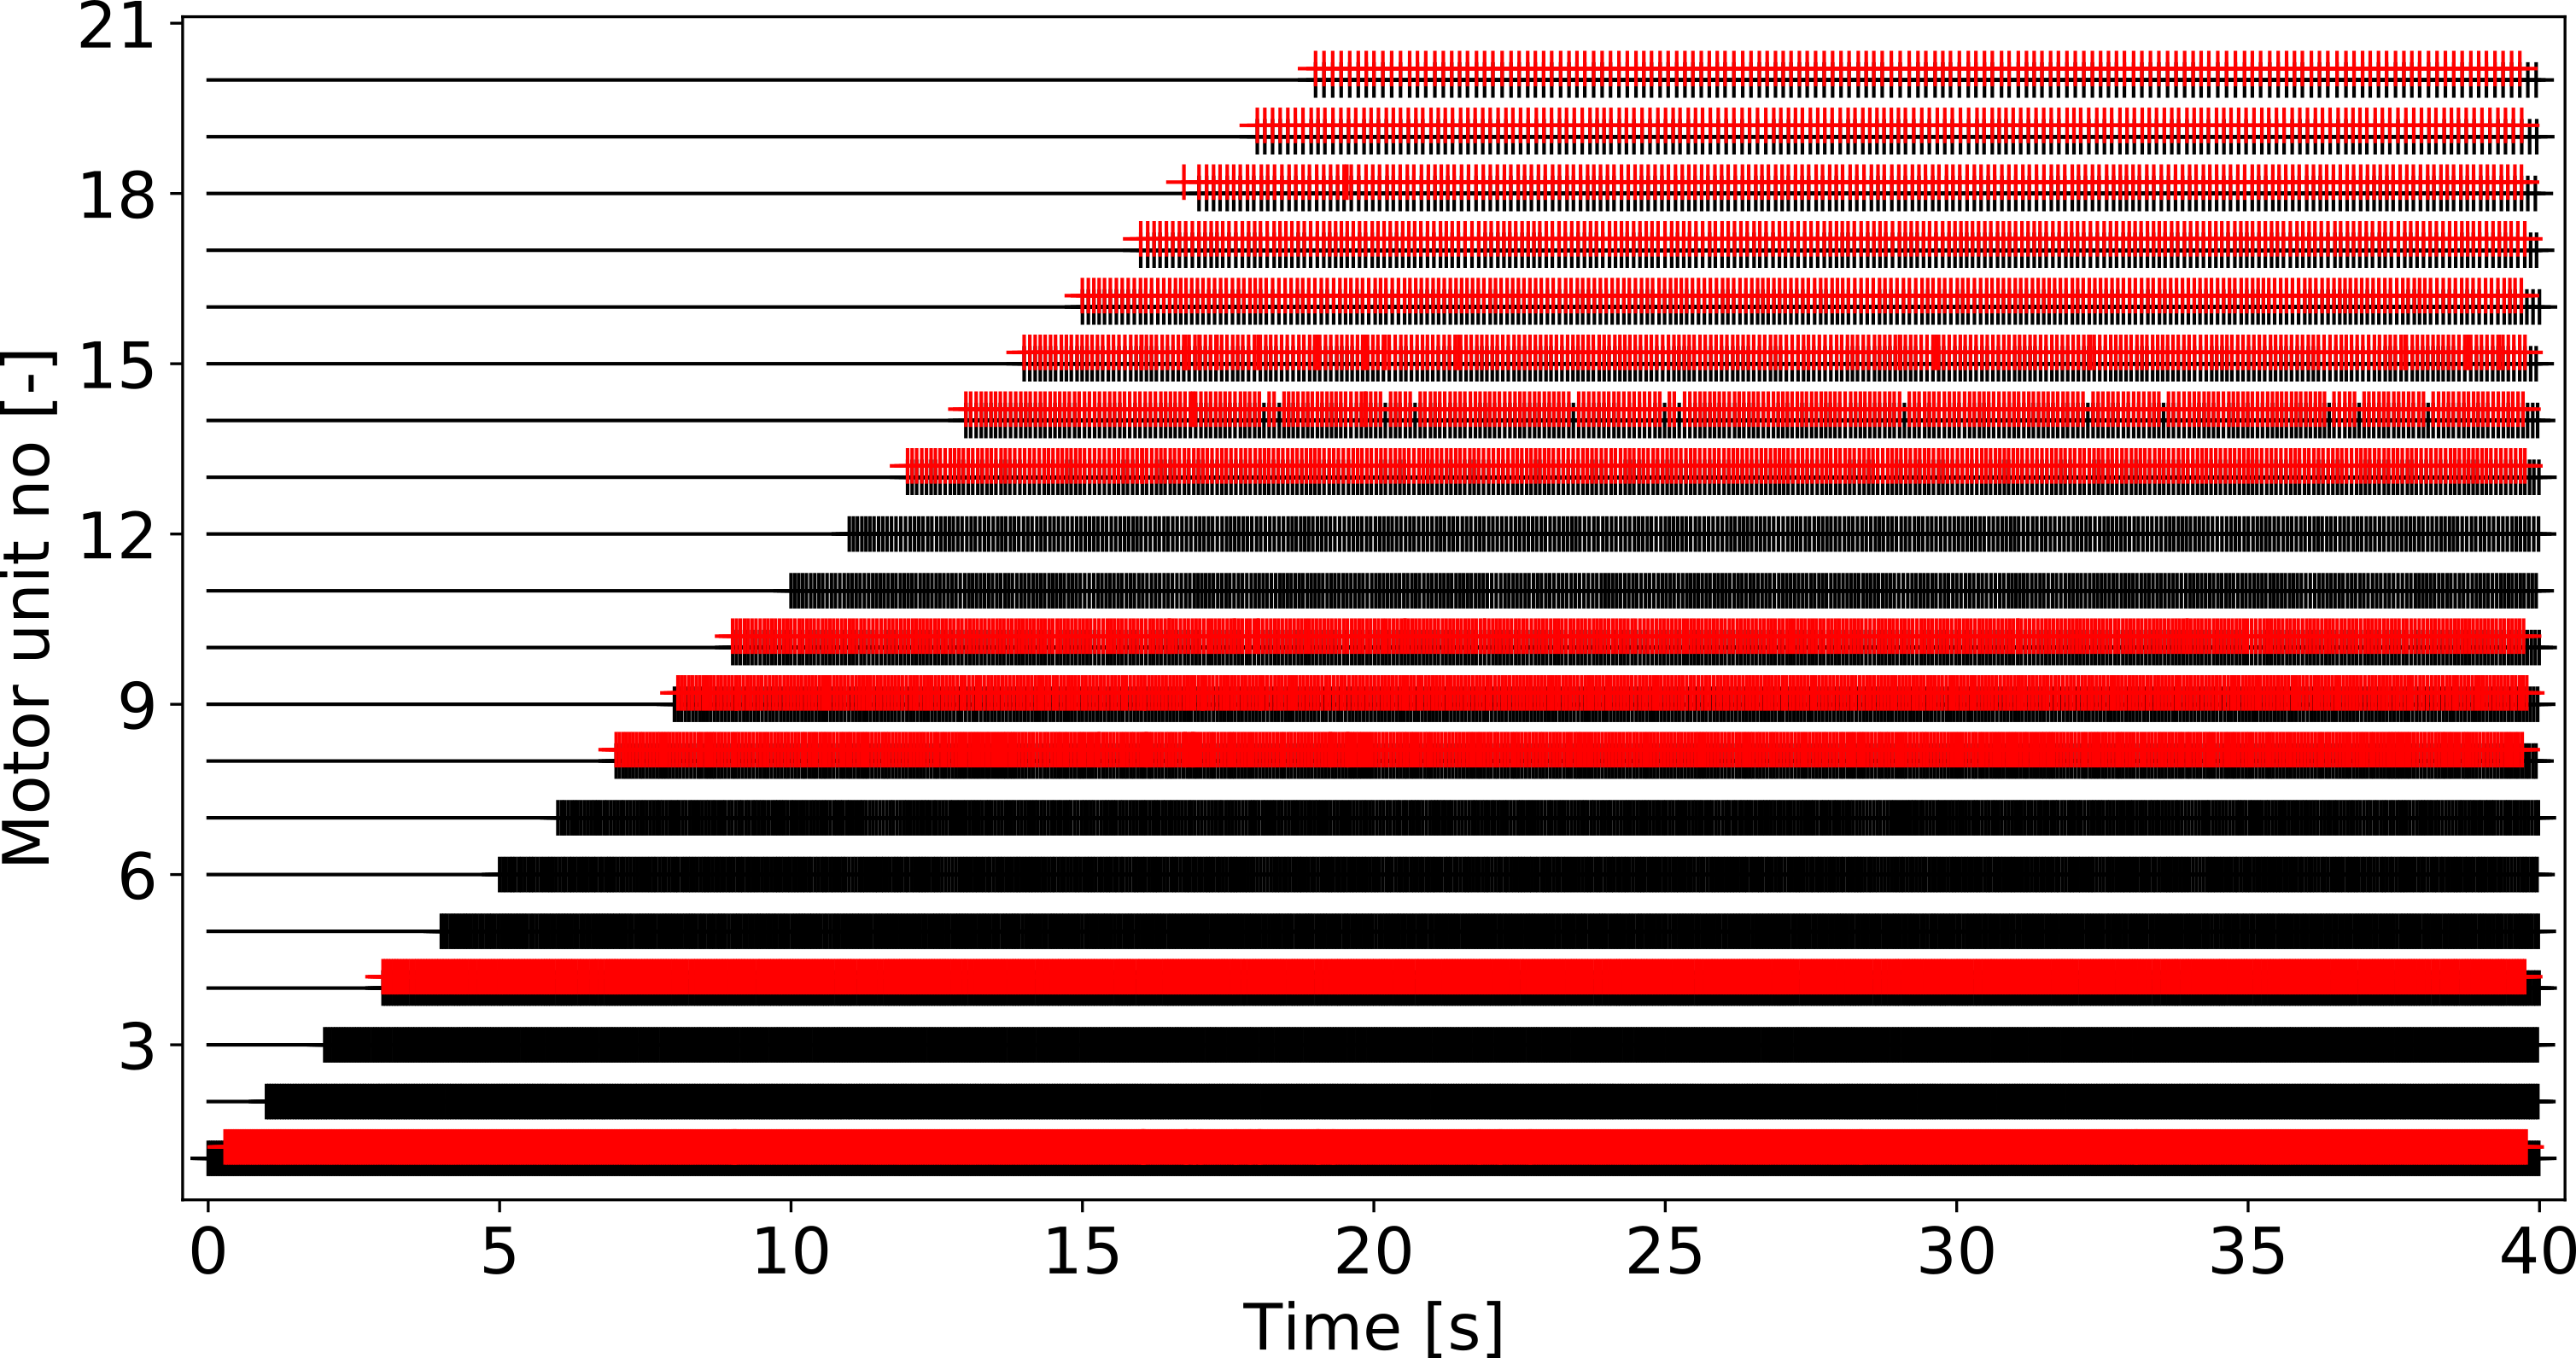
\includegraphics[width=\textwidth]{images/results/application/emg_20mus-40s_new3.png}% .pdf
  \caption{Validation experiment for EMG decomposition based on fiber-based simulations of the biceps bracchii muscle: Activation pattern for the second scenario with 20 MUs. The activation times used in the simulation are shown as black markers, the recovered activation pulses of the EMG decomposition algorithm are shown as red markers.}%
  \label{fig:emg_20mus-40s_new}%
\end{figure}

Moreover, another scenario with 20 MUs was computed, but the fat layer was varied to have a thickness of only \SI{2}{\mm} instead of \SI{1}{\cm}. In addition, the association scheme between MUs and fibers was changed to the one shown in \cref{fig:newmus}. The exponential distribution of MU sizes only varied between 42 and 102 fibers per MU, corresponding to a basis in the exponential function of approximately $1.05$ instead of $1.2$.

\Cref{fig:emg_20mus-40s_new} shows the results of the EMG decomposition with the gCKC algorithm for this second scenario with 20 MUs. DEMUSE successfully decomposed the signal into 13 MUs, corresponding to \SI{65}{\percent} of the 20 simulated MUs. DEMUSE also determined two additional MUs, which we do not consider part of the set of successfully recovered MUs. The first dataset only consists of ten innervation pulses, and the second pulse train contains high frequency oscillations.
In this scenario, the software marked only one EMG recording channel as invalid, which means that more data were considered by the decomposition algorithm than in the first scenario with 20 MUs.

Similar to the previously presented scenario, the larger MUs were detected with a higher probability than the smaller MUs. In this scenario, the eight largest MUs were successfully found. 
\Cref{fig:newmus_2d} shows the spatial arrangement of the detected MUs. The area of the muscle cross section that is occupied by undetected MUs is again located more distantly to the skin surface at the upper boundary. However, the recovered MUs 1 and 14 are nevertheless located at the lower boundary, i.e., in the most distant area from the EMG electrodes. 

%-----

% time shifts
\begin{figure}
  \centering%
  \begin{subfigure}[t]{0.47\textwidth}%
    \centering%
    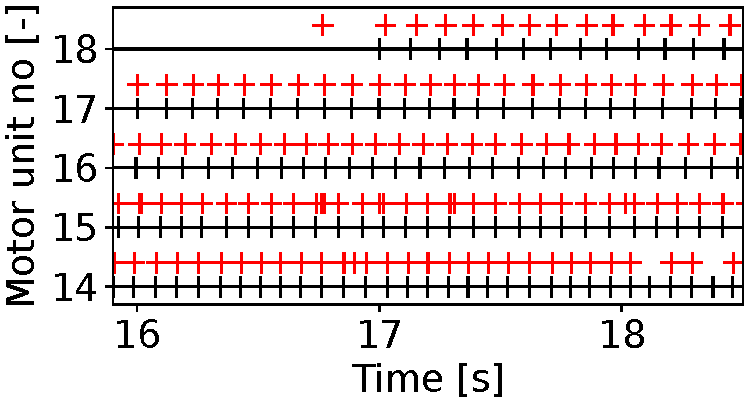
\includegraphics[width=\textwidth]{images/results/application/emg_20mus-40s_new-noshift2.pdf}%
    \caption{Original data, where a constant time shift between the simulated (black) and recovered (red) markes can be seen, especially for MUs 16 and 18.}%
    \label{fig:newmus_nocorrection}%
  \end{subfigure}
  \hfill
  \begin{subfigure}[t]{0.47\textwidth}%
    \centering%
    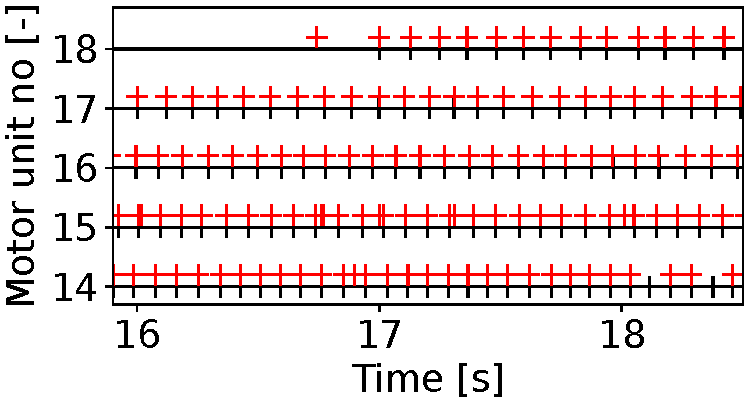
\includegraphics[width=\textwidth]{images/results/application/emg_20mus-40s_new-shift2.pdf}%
    \caption{Same data as in (a) with applied time offset correction. The applied time shifts for MUs 16 and 18 are \SI{-12.9}{\ms} and \SI{-24.9}{\ms}, respectively.}%
    \label{fig:newmus_withcorrection}%
  \end{subfigure}
  \caption{Validation experiment for EMG decomposition based on fiber-based simulations of the biceps bracchii muscle: Excerpts of the detected firing times of MUs 14 to 18 in the second scenario with 20MUs. The stimulation times of the simulation are given by black markers, the recovered times are visualized by red crosses.}%
  \label{fig:newmus_shifting}%
\end{figure}

Next, we evaluate the quality of the innervation pulse trains that were recovered by the gCKC algorithm in our scenarios. We compare the stimulation times calculated by DEMUSE with the stimulation times of the simulation. \Cref{fig:newmus_nocorrection} shows an excerpt of the detected pulse trains of the second scenario with 20 MUs in \cref{fig:emg_20mus-40s_new}, where the gCKC algorithm recovered 13 MUs.  For same MUs, we observe that the recovered stimulation times are consistently shifted in time. This effect is especially visible for MUs 16 and 18. 

The reference times given by the black markers in \cref{fig:newmus_nocorrection} correspond to the times when the fibers were stimulated in the simulation in OpenDiHu. The detected MU activations in DEMUSE, however, correspond to the times when the MU action potential shapes in the EMG recording reached their maximum.
Moreover, the exact times when particular MUs reach particular EMG electrodes  depend on the distance of the electrodes to the innervation points of the MUs. The further the electrodes are away from the neuromuscular junctions along the muscle, the higher is the delay of the recorded spikes to the corresponding innervation pulses. Thus, the constant time shifts in the pulses detected by the gCKC algorithm are valid and have to be accounted for in the evaluation of the decomposition performance.

We correct for these time shifts by adding constant time offsets $\Delta t_k$ to the recovered innervation pulse trains. For every MU $k$, the algorithm finds the matching pairs of simulated and recovered pulses and optimizes the value of $\Delta t_k$ such that the time differences in these pairs after shift correction get minimal.

\Cref{fig:newmus_withcorrection} shows the same extract of MU activity as in \cref{fig:newmus_nocorrection} with applied time offsets. The time offsets for MUs 14 to 18 in this example are given as
\begin{align*}
    \Delta t_{14}&=\SI{-2.4}{\ms}, & \Delta t_{15}&=\SI{-1.1}{\ms}, & \Delta t_{16}&=\SI{-12.9}{\ms},\\
    \Delta t_{17}&=\SI{-2.9}{\ms}, \quad \text{and} & \Delta t_{18}&=\SI{-24.9}{\ms}.
\end{align*}
\Cref{fig:newmus_withcorrection} shows that the recovered pulses now match the simulated data very well. The non-matching pulses are clearly false positive detections.

To compare the recovered MU times between the scenarios, we evaluate metrics such as the rate of agreement. The MU firing times in the simulation serve as the ground truth, to which we compare the recovered MU times. We identify true positive (TP), false positive (FP) and false negative (FN) recovered pulses, depending on whether a matching time to a recovered pulse can or cannot be found in the simulation data within a tolerance of $\eps=\SI{5}{\ms}$. The rate of agreement (RoA) between the gCKC algorithm output and the ground truth data is then computed by%
\begin{align*}
  \textrm{RoA}  = \dfrac{\textrm{TP}}{\textrm{TP} + \textrm{FP} + \textrm{FN}}.
\end{align*}

In the first scenario with 20 MUs in \cref{fig:emg_20mus-50s-old2}, the RoA for MUs 16,18 and 19 is above $\SI{99.7}{\percent}$ and slightly lower at $\SI{82.2}{\percent}$ for MU 20. Here, only 296 of the 334 detected pulses were true positives, corresponding to a precision of $\SI{88.6}{\percent}$.
% MU 16 from matlab: FP: 0, TP: 484, FN: 0 -> RoA: 1.0
% MU 18 from matlab: FP: 1, TP: 409, FN: 0 -> RoA: 0.9975609756097561
% MU 19 from matlab: FP: 1, TP: 370, FN: 0 -> RoA: 0.9973045822102425
% MU 20 from matlab: FP: 38, TP: 296, FN: 26 -> RoA: 0.822222222222222
 
In the second scenario with 20 MUS presented in \cref{fig:emg_20mus-40s_new}, all valid MUs except one have RoA values of above $\SI{94.5}{\percent}$. Five MUs are even detected perfectly with $\SI{100}{\percent}$ rate of agreement. MU 9 is the only detected MU with a degraded RoA of approximately $\SI{57.9}{\percent}$. However, the RoA improves to $\SI{98.1}{\percent}$, if the tolerance $\eps$ for matching pulses is relaxed to $\SI{10}{\ms}$. This shows that the RoA metric also depends on a proper value for the tolerance $\eps$, and that some of the innervation pulse trains detected by DEMUSE can have varying accuracy in a range of less than $\SI{10}{\ms}$.
 
 %MU 9 from matlab: FP: 191, TP: 321, FN: 42 -> RoA: 0.5794223826714802
 
While the gCKC algorithm can be used for EMG decomposition of previously recorded signals in a controlled environment, it is less suited for real-time applications. The separation vectors that decompose the electrode signals and infer the MU innervation pulse trains can be computed in a training phase. 
However, their application on new data requires a certain history of previously captured signals to calculate the decomposed MU pulses. As a consequence, the predictions are delayed, which is usually undesirable in real-time applications. Furthermore, the system is sensitive to noisy data. 

A fundamentally different approach to EMG decomposition is the use of sequence-to-sequence learning methods provided by recurrent neural networks. The authors of \cite{Clarke2021} used a gated recurrent unit (GRU) network for this task. The network was trained using the output of the gCKC algorithm and was subsequently able to decompose surface EMG signals into innervation pulse trains. The approach was shown to be robust and to outperform gCKC for low signal-to-noise ratios.

To assess, whether our simulations of surface EMG can be used for the supervised learning of GRU networks for EMG decomposition, we tried in a first step to reproduce the studies of \cite{Clarke2021}, where the GRU is trained with the output of the gCKC algorithm. Additionally, we trained a GRU network directly on the simulated EMG data. These tasks were carried out in the masters project of Srijay Kolvekar and were supervised by Lena Lehmann and me. For details on the methods and results, we refer to the literature \cite{Clarke2021} and the project report \cite{Srijay}.

In this project, the EMG decomposition of a GRU network trained with raw innervation pulse trains obtained from the gCKC algorithm, similar to the literature, showed a large number of false positive and false negative predictions.
However, a different setup using MU labels instead of raw pulse trains showed promising results. 
Every discrete point in time (according to the EMG sampling frequency) was either associated with the class of the currently active MU or with the background class, when no MU was activated at the time. This classification problem had a large class imbalance, as the background class was active for \SI{86}{\percent} of the timesteps. The issue was mitigated by using class weights. The GRU network was trained with simulation data and yielded per-class rates of agreement of up to \SI{72}{\percent} for the two scenarios with 20 MUs shown in \cref{fig:emg_20mus-50s-old2,fig:emg_20mus-40s_new}, i.e., with the test data set also generated by our simulation.

\Cref{fig:gru_result} presents an excerpt of the resulting predictions of a GRU network that was trained with simulation results.
We used the simulation of the second scenario with 20 MUs, which is shown in \cref{fig:emg_20mus-40s_new}. 
The black markers in \cref{fig:gru_result} indicate the stimulation times used in the simulation. 
The red markers correspond to the recovered times by the gCKC algorithm. 
Out of the shown MUs, only MUS 9 and 10 were recovered by the gCKC algorithm.
The blue markers denote the GRU predictions. Correction of time offsets was performed for both the gCKC and GRU outputs.

\Cref{fig:gru_result} shows the best agreement between the two prediction methods for MU 10 with a RoA of \SI{99.6}{\percent} for the gCKC algorithm and \SI{72.2}{\percent} for the GRU network. In contrast to the gCKC algorithm, the GRU network predicts firings for all MUs. However, the quality is only acceptable for MUs that could also be detected by the gCKC algorithm. For MUs 11 and 12, the RoA for the GRU network is around \SI{30}{\percent}.

In future work, the decomposition performance of the GRU networks could be improved by using different training data. For example, the ramp activation in the training data could be replaced by constant tetanic stimulations. Moreover, different network architectures, such as convolutional recurrent neural networks could be investigated.

\begin{figure}
  \centering%
  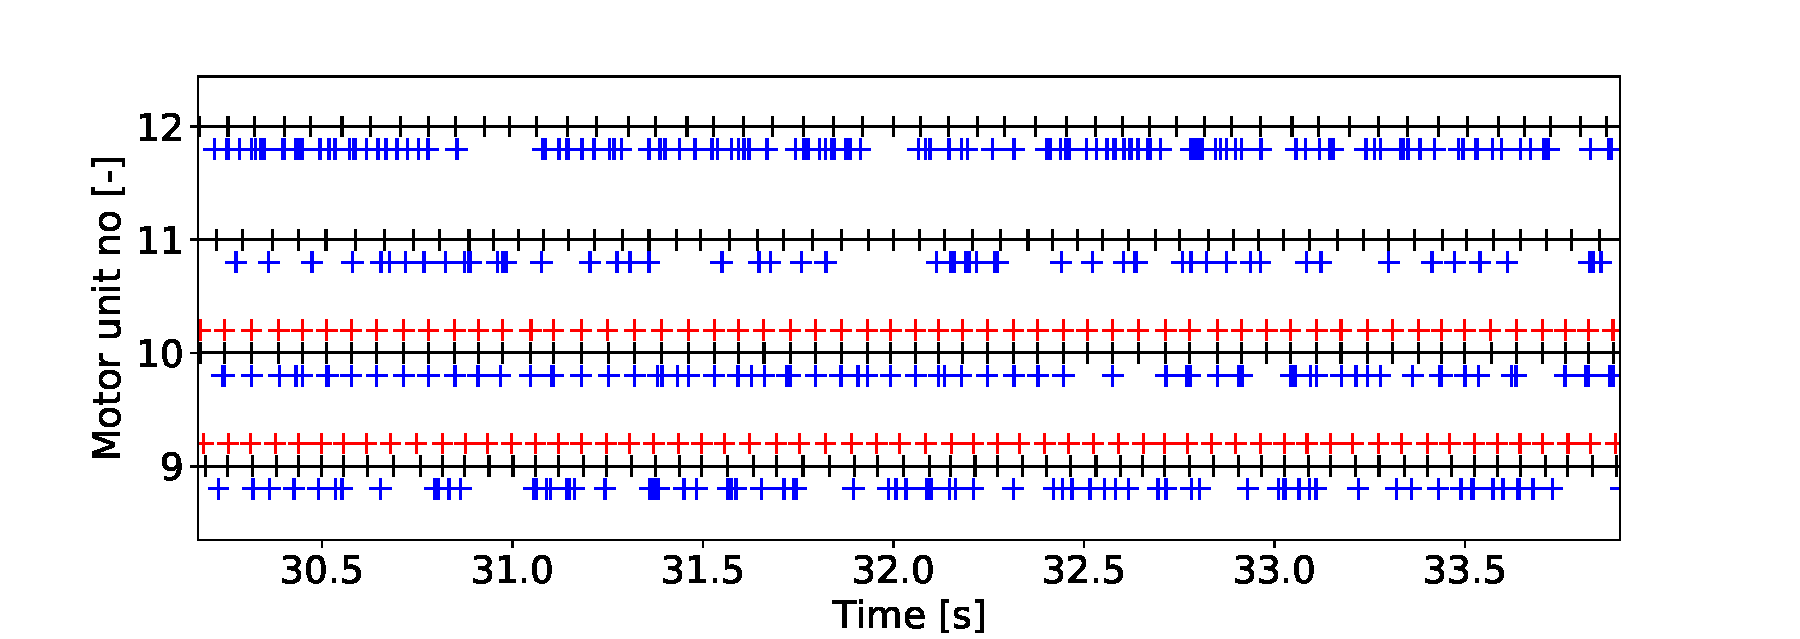
\includegraphics[width=\textwidth]{images/results/application/gru2.pdf}%
  \caption{Comparison of innervation pulse train predictions of the gCKC algorithm (red), a GRU network (blue) and the ground truth data (black).}%
  \label{fig:gru_result}%
\end{figure}

 %MU 1 from gru: FP: 411, TP: 536, FN: 92 -> RoA: 0.5158806544754572
 %MU 2 from gru: FP: 458, TP: 513, FN: 27 -> RoA: 0.5140280561122245
 %MU 3 from gru: FP: 698, TP: 877, FN: 50 -> RoA: 0.5396923076923077
 %MU 4 from gru: FP: 252, TP: 503, FN: 42 -> RoA: 0.6311166875784191
 %MU 5 from gru: FP: 708, TP: 469, FN: 15 -> RoA: 0.3934563758389262
 %MU 6 from gru: FP: 705, TP: 691, FN: 52 -> RoA: 0.47720994475138123
 %MU 7 from gru: FP: 308, TP: 566, FN: 24 -> RoA: 0.6302895322939867
 %MU 8 from gru: FP: 469, TP: 290, FN: 84 -> RoA: 0.34400948991696323
 %MU 9 from gru: FP: 342, TP: 182, FN: 52 -> RoA: 0.3159722222222222
 %MU 10 from gru: FP: 94, TP: 293, FN: 19 -> RoA: 0.7216748768472906
 %MU 11 from gru: FP: 215, TP: 142, FN: 70 -> RoA: 0.3325526932084309
 %MU 12 from gru: FP: 671, TP: 295, FN: 61 -> RoA: 0.2872444011684518
 %MU 13 from gru: FP: 576, TP: 208, FN: 27 -> RoA: 0.2564734895191122
 %MU 14 from gru: FP: 418, TP: 155, FN: 1 -> RoA: 0.2700348432055749
 %MU 15 from gru: FP: 299, TP: 112, FN: 55 -> RoA: 0.24034334763948498
 %MU 16 from gru: FP: 234, TP: 122, FN: 62 -> RoA: 0.291866028708134
 %MU 17 from gru: FP: 85, TP: 131, FN: 21 -> RoA: 0.5527426160337553
 %MU 18 from gru: FP: 302, TP: 60, FN: 65 -> RoA: 0.1405152224824356
 %MU 19 from gru: FP: 65, TP: 53, FN: 51 -> RoA: 0.3136094674556213
 %MU 20 from gru: FP: 71, TP: 18, FN: 56 -> RoA: 0.12413793103448276

In conclusion, the gCKC algorithm is able to decompose artifically generated surface EMG signals. This means that our simulation can be used to evaluate the performance of EMG decomposition algorithms.

The number of detected MUs depends on the relation between MU sizes and on the distance of the MU territories to the electrodes. If the variance of the sizes of the activated MUs is small, such as in \cref{fig:newmus_progression}, also MUs that are far away from the electrodes are detected. If, in the opposite case, the sizes of active MUs are distributed over a large range such as in \cref{fig:oldmus_progression}, only the largest MUs are detectable.

In addition, the amount of adipose tissue between the electrodes and the muscle influences the number of MUs that can be recovered. In our studies, the performance of EMG decomposition was lower for all scenarios with thicker fat layer than for the scenario with a thin fat layer.

The rate of agreement of the determined pulse trains of the DEMUSE software was above $\SI{95}{\percent}$ in most of the cases. Correspondingly, the rate of false positives was low.
A time shift between the recovered times and the ground truth data was observed for some pulse trains, which can be explained with the delay from first activation to the onset of the EMG signal. As a result, the time shift was corrected for the rate of agreement measurement.

A proof-of-concept implementation of GRU networks showed promising performance for predicting MU firing times from artifical EMG recordings. 
The GRU network predicted firing times also for MUs that were not detected by the gCKC algorithm, however the rate of agreement was low for these MUs.
In future work, the GRU decomposition method has to be refined to be comparative to the gCKC algorithm.

% Satz einfügen, dass die GRU networks immerhin in der Lage waren, mehr MUs als gCKC zu identifizieren, allerdings die firing times nicht sehr gut getroffen wurden.

% new
%End time: 39.9988, number of motor units: 20, number of fibers: 1369

%Try to load and process data from matlab file "emg_results.mat"
%Discard MU no. 13 from matlab file with onset time 0.456s
%Discard MU no. 14 from matlab file with onset time 9.0125s
 %MU 1 from matlab: FP: 40, TP: 943, FN: 3 -> RoA: 0.9563894523326572
 %MU 4 from matlab: FP: 0, TP: 768, FN: 0 -> RoA: 1.0
 %MU 9 from matlab: FP: 191, TP: 321, FN: 42 -> RoA: 0.5794223826714802
 %MU 8 from matlab: FP: 6, TP: 552, FN: 0 -> RoA: 0.989247311827957
 %MU 10 from matlab: FP: 2, TP: 470, FN: 0 -> RoA: 0.9957627118644068
 %MU 13 from matlab: FP: 1, TP: 346, FN: 0 -> RoA: 0.9971181556195965
 %MU 16 from matlab: FP: 0, TP: 248, FN: 0 -> RoA: 1.0
 %MU 17 from matlab: FP: 0, TP: 222, FN: 0 -> RoA: 1.0
 %MU 14 from matlab: FP: 2, TP: 303, FN: 0 -> RoA: 0.9934426229508196
 %MU 15 from matlab: FP: 16, TP: 280, FN: 0 -> RoA: 0.9459459459459459
 %MU 18 from matlab: FP: 2, TP: 194, FN: 0 -> RoA: 0.9897959183673469
 %MU 19 from matlab: FP: 0, TP: 168, FN: 0 -> RoA: 1.0
 %MU 20 from matlab: FP: 0, TP: 145, FN: 0 -> RoA: 1.0

%Try to load and process data from GRU file "ipt_prediction.csv"
%Could not load data from a GRU file "ipt_prediction.csv".
%Traceback (most recent call last):
  %File "/store/software/opendihu/scripts/plot_stimulation_log.py", line 266, in <module>
    %with open(gru_filename, "r") as f:
%FileNotFoundError: [Errno 2] No such file or directory: 'ipt_prediction.csv'
%MU  1 ground truth, onset: 0.000 s, frequency: 24.42 Hz
             %matlab onset: 0.277 s, frequency: 24.39 Hz (timeshift: 0.01270s), RoA: 0.956, data end: 39.7585 s
%MU  2 ground truth, onset: 1.000 s, frequency: 22.52 Hz
%MU  3 ground truth, onset: 2.000 s, frequency: 21.83 Hz
%MU  4 ground truth, onset: 3.000 s, frequency: 20.91 Hz
             %matlab onset: 3.003 s, frequency: 20.83 Hz (timeshift: -0.00300s), RoA: 1.000, data end: 39.749 s
%MU  5 ground truth, onset: 4.000 s, frequency: 19.96 Hz
%MU  6 ground truth, onset: 5.000 s, frequency: 18.59 Hz
%MU  7 ground truth, onset: 6.000 s, frequency: 17.70 Hz
%MU  8 ground truth, onset: 7.000 s, frequency: 16.84 Hz
             %matlab onset: 7.007 s, frequency: 16.95 Hz (timeshift: -0.00700s), RoA: 0.989, data end: 39.7105 s
%MU  9 ground truth, onset: 8.000 s, frequency: 16.10 Hz
             %matlab onset: 8.033 s, frequency: 16.13 Hz (timeshift: 0.02690s), RoA: 0.579, data end: 39.754 s
%MU 10 ground truth, onset: 9.000 s, frequency: 15.18 Hz
             %matlab onset: 9.014 s, frequency: 15.15 Hz (timeshift: -0.01690s), RoA: 0.996, data end: 39.7435 s
%MU 11 ground truth, onset: 10.000 s, frequency: 14.43 Hz
%MU 12 ground truth, onset: 11.000 s, frequency: 13.28 Hz
%MU 13 ground truth, onset: 12.000 s, frequency: 12.45 Hz
             %matlab onset: 12.002 s, frequency: 12.50 Hz (timeshift: -0.00270s), RoA: 0.997, data end: 39.7515 s
%MU 14 ground truth, onset: 13.000 s, frequency: 11.91 Hz
             %matlab onset: 13.002 s, frequency: 11.87 Hz (timeshift: -0.00240s), RoA: 0.993, data end: 39.719 s
%MU 15 ground truth, onset: 14.000 s, frequency: 10.86 Hz
             %matlab onset: 14.001 s, frequency: 10.99 Hz (timeshift: -0.00110s), RoA: 0.946, data end: 39.752 s
%MU 16 ground truth, onset: 15.000 s, frequency: 10.00 Hz
             %matlab onset: 15.011 s, frequency: 10.00 Hz (timeshift: -0.01290s), RoA: 1.000, data end: 39.701 s
%MU 17 ground truth, onset: 16.000 s, frequency: 9.32 Hz
             %matlab onset: 16.003 s, frequency: 9.35 Hz (timeshift: -0.00290s), RoA: 1.000, data end: 39.75 s
%MU 18 ground truth, onset: 17.000 s, frequency: 8.53 Hz
             %matlab onset: 16.766 s, frequency: 8.51 Hz (timeshift: -0.02490s), RoA: 0.990, data end: 39.7155 s
%MU 19 ground truth, onset: 18.000 s, frequency: 7.67 Hz
             %matlab onset: 18.002 s, frequency: 7.66 Hz (timeshift: -0.00170s), RoA: 1.000, data end: 39.696 s
%MU 20 ground truth, onset: 19.000 s, frequency: 6.97 Hz
             %matlab onset: 19.003 s, frequency: 6.97 Hz (timeshift: -0.00360s), RoA: 1.000, data end: 39.6655 s
%Matlab file "emg_results.mat" contains 13 matching MUs, 2 discarded.


% End time: 49.9945, number of motor units: 20, number of fibers: 1369
% Try to load and process data from matlab file "emg_results.mat"
%  MU 16 from matlab: FP: 0, TP: 484, FN: 0 -> RoA: 1.0
%  MU 18 from matlab: FP: 1, TP: 409, FN: 0 -> RoA: 0.9975609756097561
%  MU 19 from matlab: FP: 1, TP: 370, FN: 0 -> RoA: 0.9973045822102425
%  MU 17 from matlab: FP: 306, TP: 28, FN: 109 -> RoA: 0.06320541760722348
% 
% 
% End time: 49.9961, number of motor units: 50, number of fibers: 1369
% Try to load and process data from matlab file "emg_results.mat"
% Discard MU no. 8 from matlab file with onset time 45.1375s
%  MU 29 from matlab: FP: 26, TP: 521, FN: 0 -> RoA: 0.9524680073126143
%  MU 48 from matlab: FP: 4, TP: 301, FN: 0 -> RoA: 0.9868852459016394
%  MU 45 from matlab: FP: 5, TP: 321, FN: 0 -> RoA: 0.9846625766871165
%  MU 41 from matlab: FP: 1, TP: 373, FN: 0 -> RoA: 0.9973262032085561
%  MU 50 from matlab: FP: 4, TP: 283, FN: 0 -> RoA: 0.9860627177700348
%  MU 43 from matlab: FP: 15, TP: 350, FN: 0 -> RoA: 0.958904109589041
%  MU 42 from matlab: FP: 46, TP: 330, FN: 6 -> RoA: 0.8638743455497382
%  MU 44 from matlab: FP: 5, TP: 165, FN: 25 -> RoA: 0.8461538461538461
% 
% % 
% % 
% % 
% End time: 36.9988, number of motor units: 100, number of fibers: 4489
% 
% Try to load and process data from matlab file "emg_results.mat"
%  MU 63 from matlab: FP: 320, TP: 47, FN: 118 -> RoA: 0.09690721649484536
%  MU 81 from matlab: FP: 0, TP: 292, FN: 0 -> RoA: 1.0
%  MU 40 from matlab: FP: 18, TP: 478, FN: 0 -> RoA: 0.9637096774193549
%  MU 83 from matlab: FP: 253, TP: 17, FN: 141 -> RoA: 0.0413625304136253
%  MU 100 from matlab: FP: 3, TP: 242, FN: 0 -> RoA: 0.9877551020408163
%  MU 95 from matlab: FP: 6, TP: 250, FN: 3 -> RoA: 0.9652509652509652
%  MU 97 from matlab: FP: 0, TP: 250, FN: 0 -> RoA: 1.0
%  MU 84 from matlab: FP: 16, TP: 282, FN: 0 -> RoA: 0.9463087248322147
%  MU 99 from matlab: FP: 0, TP: 243, FN: 0 -> RoA: 1.0
%  MU 90 from matlab: FP: 217, TP: 20, FN: 116 -> RoA: 0.056657223796033995
%  MU 15 from matlab: FP: 789, TP: 180, FN: 90 -> RoA: 0.16997167138810199
%  MU 87 from matlab: FP: 209, TP: 93, FN: 48 -> RoA: 0.26571428571428574
% 
% 

% t=100ms

% ----------
%\fi
% ===========f

% ==================
%\iffalse
% =-------------------

\subsection{Simulation of Electrophysiology with a Phenomenological Fiber Model}\label{sec:sim_rosenfalck}

Instead of the previously presented numeric model of action potential propagation on the muscle fibers, the respective physiological process can also be described with a phenomenological approach.

The model formulated by Rosenfalck \cite{Rosenfalck1969} describes the action potential shape on a 1D domain by the following function:
%
\begin{align*}
  G(z) = \begin{cases}
    96\,z^3\,\exp(-z) - 9 & \text{for } z \geq 0,\\[4mm]
    -90  & \text{for } z < 0.
  \end{cases}  
\end{align*}

\begin{figure}
  \centering%
  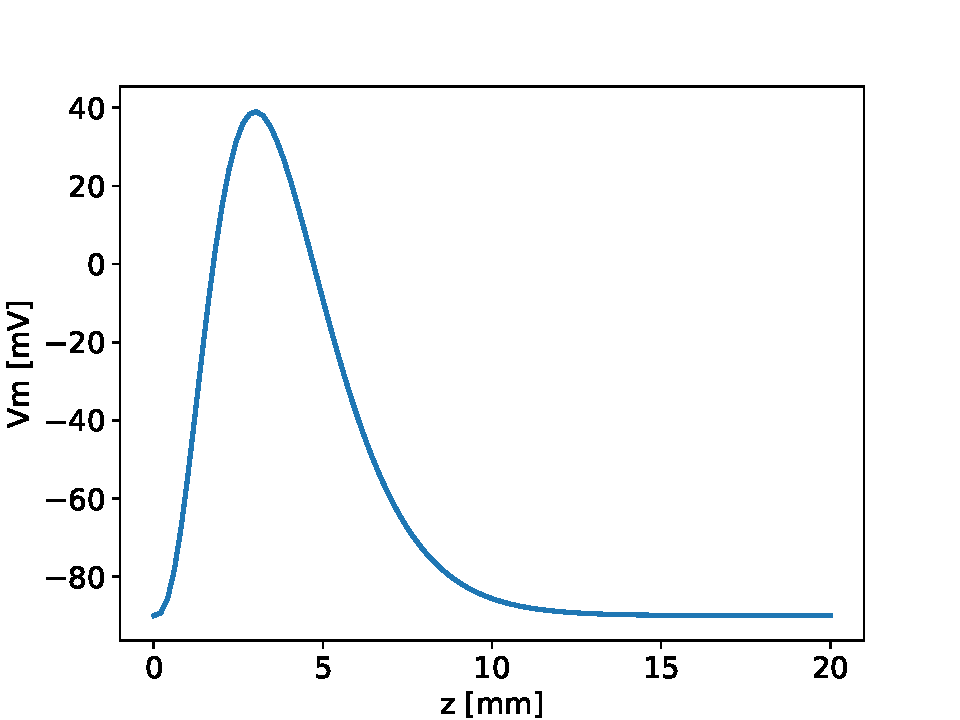
\includegraphics[width=0.6\textwidth]{images/results/application/rosenfalck_function.pdf}%
  \caption{Simulation of EMG signals on the upper arm; analytic model by Rosenfalck of an action potential shape on a 1D fiber.}%
  \label{fig:rosenfalck_function}%
\end{figure}
\Cref{fig:rosenfalck_function} shows the graph of this function. The resulting value of $G$ specifies the membrane voltage in millivolts. The coordinate $z=x+v\,t$ depends on the distance $x$ to the neuromuscular junction on the fiber, the conduction velocity $v$ and the time $t$ after the last stimulation. In our simulation, we use the proposed propagation velocity of \SI{4}{\meter\per\second}.

The advantage of using an analytic model is its fast calculation runtime compared with the numeric model. On the downside, such a model cannot accurately describe fatigue effects in tetanic stimulations or the action potential shape changing properties of more advanced subcellular models.

One use case of such an analytic model is to study the effect of muscle fiber arrangements in a muscle volume on the surface EMG signal. In this case, the exact, possibly time-varying shapes of the motor unit action potentials are less important than the location and orientation of the fibers.
We provide an examplary scenario in OpenDiHu, which uses the Rosenfalck model on multiple 1D muscle fibers that are embedded in a 3D domain. As in the previous sections, the 3D bidomain model given by \cref{eq:bidomain1} is coupled to the fibers and used to simulate EMG recordings on the surface. 

In addition to the simplified model of action potential propagation, we use a simplified description of the muscle geometry. \Cref{fig:custom_geometry} shows the artifical geometry, which is constructed by rotating a transformed sine curve around the $z$ axis. 
Our program embeds the fibers automatically inside the volume and orients them according to specified spherical coordinates. The orientation angles, the number of fibers and the spacings between the fibers can be adjusted in the Python settings script of the simulation.

\begin{figure}
  \centering%
  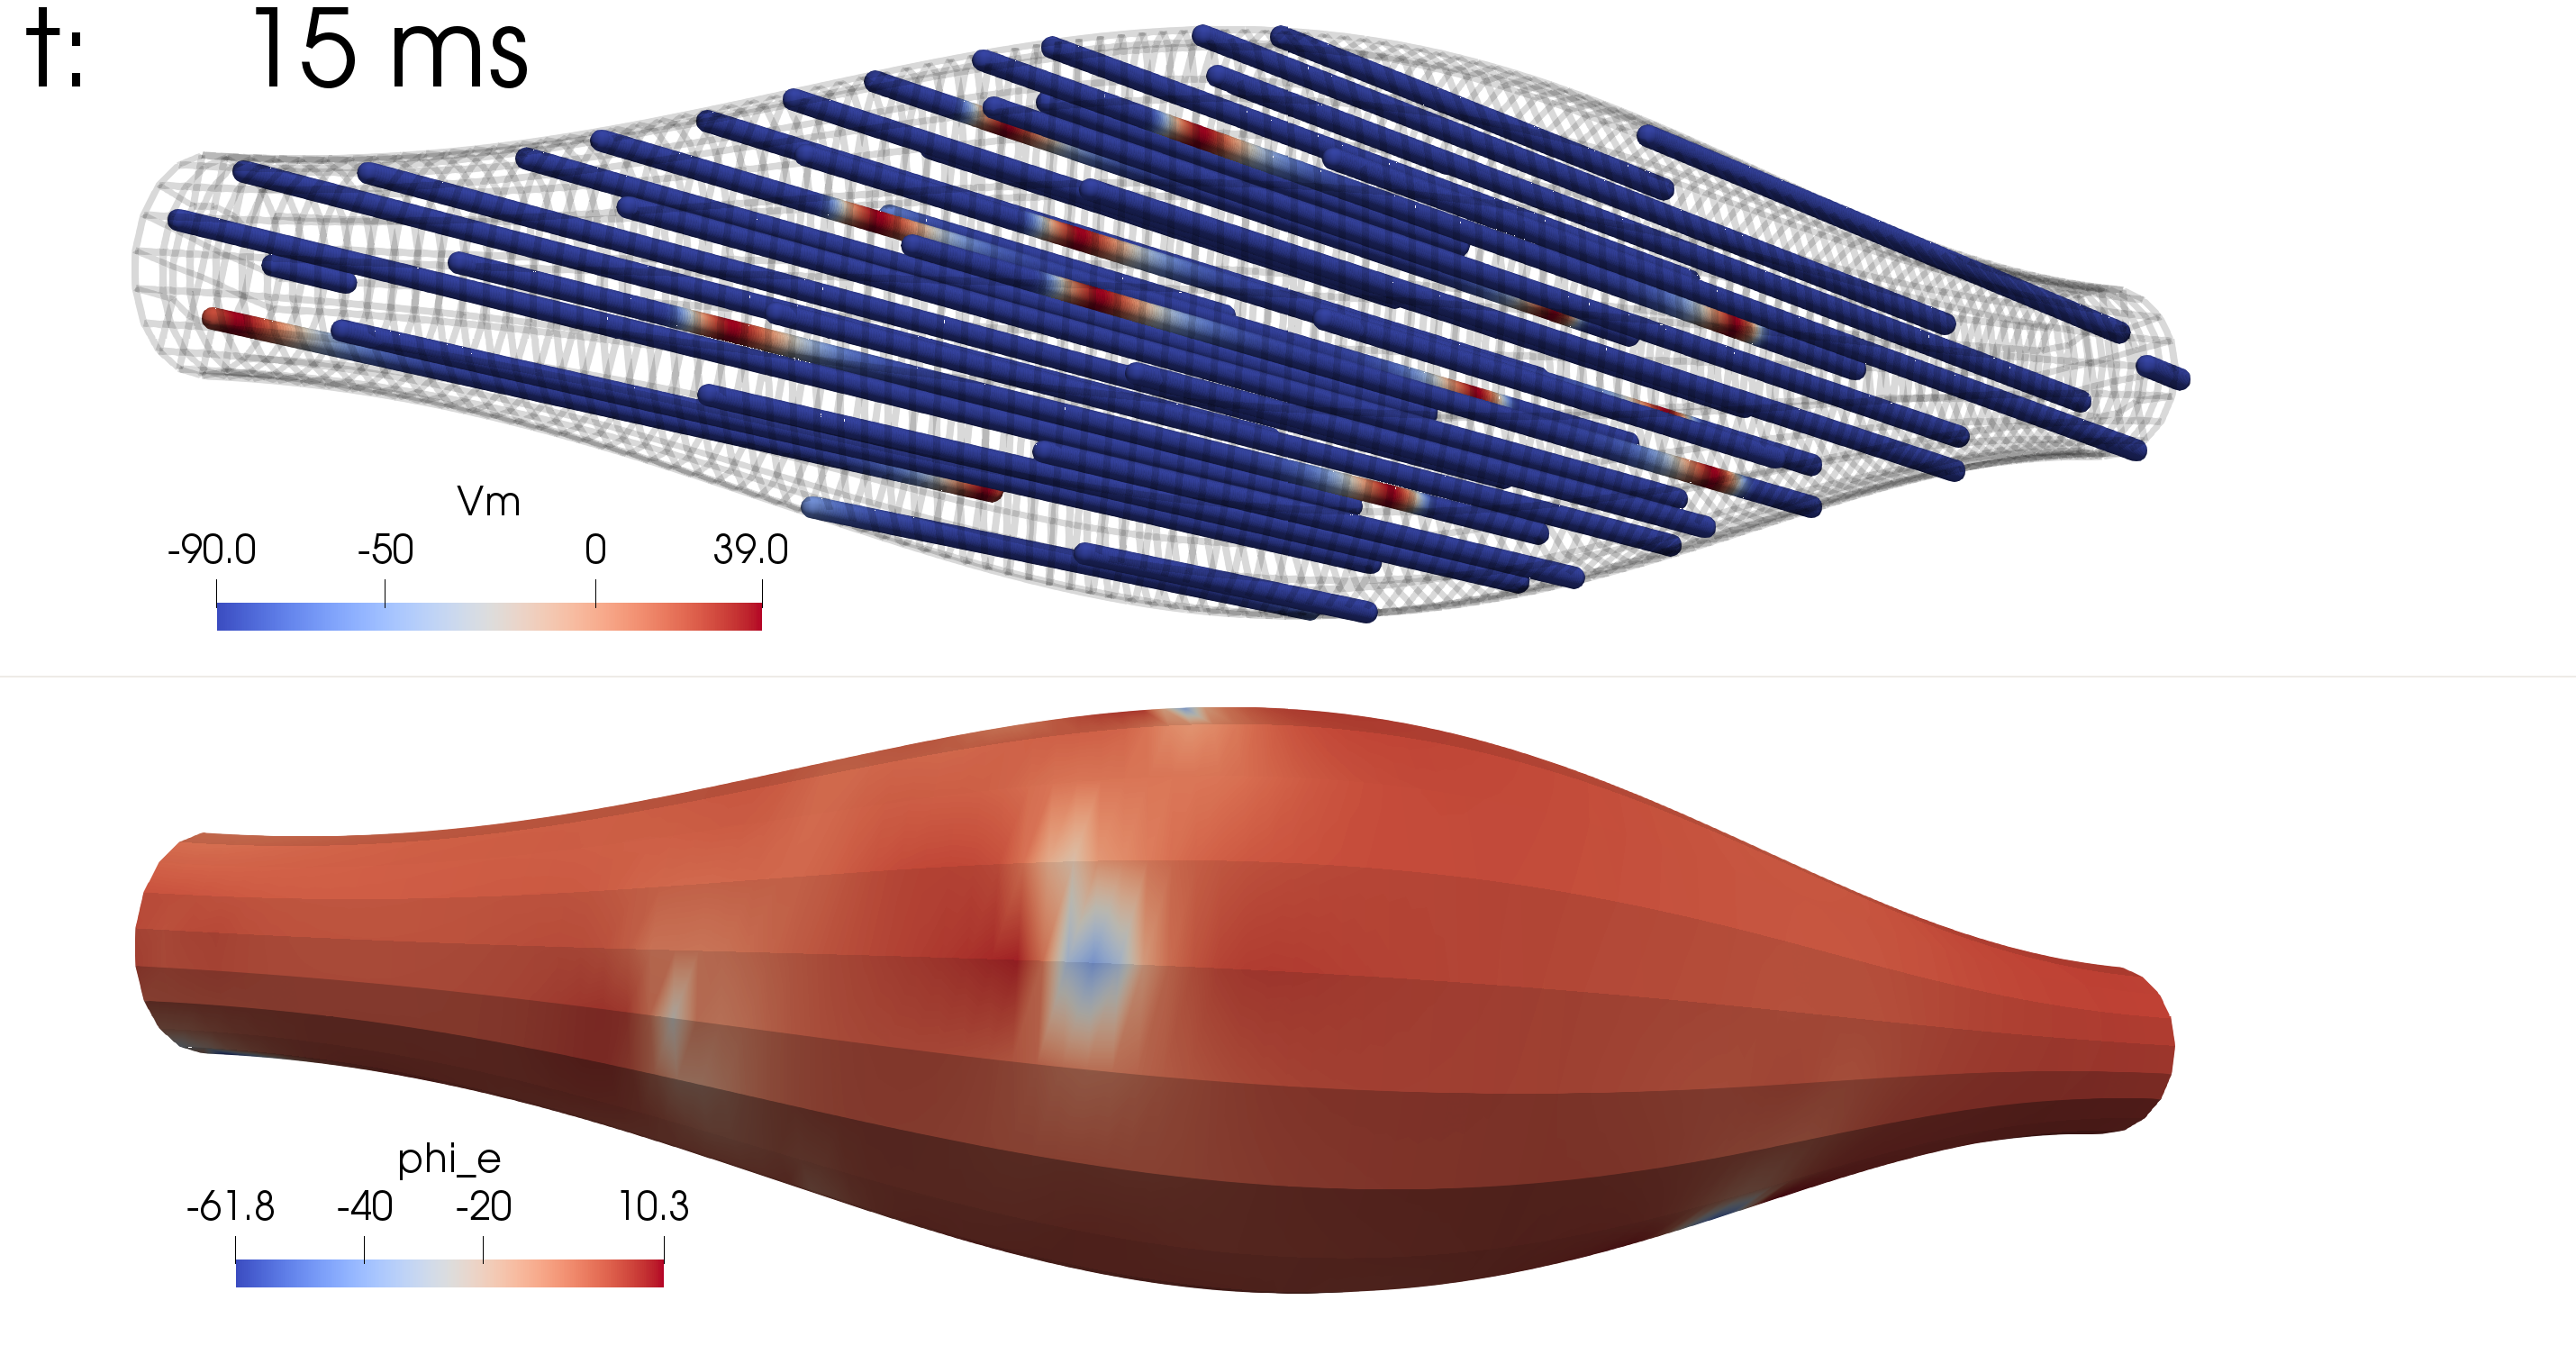
\includegraphics[width=\textwidth]{images/results/application/custom_geometry.png}%
  \caption{Simulation of EMG signals on the upper arm; artifical muscle geometry with a phenomenological model of action potential propagation. The upper image shows the muscle fibers, colored according to the transmembrane potential $V_m$. The lower image shows the extracellular potential $\phi_e$ on the surface.
  This scenario can be computed very fast and can, e.g., be useful to investigate the effects of different fiber orientations.}%
  \label{fig:custom_geometry}%
\end{figure}

\Cref{fig:custom_geometry} shows the location of the fibers inside the artificial muscle belly in the upper image and a simulation result of muscular activity  at $t=\SI{15}{\ms}$ in the lower image. The resulting EMG signal can be seen on the surface.
This simulation scenario provides means to quickly study electrophysiology and generation of EMG for a generic muscle. Solving the model only consists of evaluations of the Rosenfalck function and repeated computation of the 3D model, but no further costly computations of numeric electrophysiology models. Moreover, no mesh file has to be generated and loaded, which simplifies the handling of the scenario.

\begin{reproduce_no_break}
  The simulation in \cref{fig:custom_geometry} can be started as follows.
  \begin{lstlisting}[columns=fullflexible,breaklines=true,postbreak=\mbox{\textcolor{gray}{$\hookrightarrow$}\space}]
    cd $\$$OPENDIHU_HOME/examples/electrophysiology/fibers/analytical_fibers_emg/build_release
    ./analytical_fibers_emg ../settings_analytical_fibers_emg_custom_geometry.py geometry_round.py
  \end{lstlisting}
  The options can be set in the \code{variables/geometry_round.py} settings file. Other artifical geometries are available by using other scripts under \code{variables}.
\end{reproduce_no_break}

\subsection{Conclusion}

In the present section, surface EMG signals were computed using the fiber based electrophysiology model. We showed, how the qualitative nature of the signals depends on the spatial distribution of the MUs and that the thickness of the body fat layer influences the smoothness of the recorded EMG signals. Furthermore, we investigated the effect of the mesh resolution and the number of fibers in the simulation. The results showed that only a high mesh resolution can resolve the small features in the EMG signal  on the skin surface, which result from fiber action potentials. The number of these features in the result increased with the mesh width and, thus, the two finest discretizations with \num{77e3} \num{274e3} fibers yielded the most accurate results. As a consequence, High Performance Computing simulations are required, if an accurate 2D surface EMG signal should be computed.

Further studies with EMG decomposition algorithms showed another use case of our fiber based surface EMG simulations: They can be used as a validation tool for existing decomposition algorithms and they can serve as a data generator to develop novel, data based decomposition methods. The decomposition software DEMUSE was tested and we quantified the rate of agreement of its predictions with our simulation. Similarly, we evaluated a neural network based approach and compared its performance on the simulated data with the previous method.

%TODO, Ich fände es hier ganz gut, wenn es noch eine kleine Summary von 6.4 gäbe, die wesentlichen Fragen beantwortet: Was kann de faser-basierte Simulation für Einsichten liefern? Lohnt sich die höhere Auflösung? Inwiefern war sie nützlich zur Validierung der Zerlegungsalgorithmen für EMG-Messungen?
